\special{pdf:minorversion 7}
\PassOptionsToPackage{dvipsnames}{xcolor}
\documentclass[11pt,a4paper]{report}

\usepackage[todonotes={textsize=scriptsize}, draft]{changes}
\usepackage[left=3cm, right=3cm, top=3cm, bottom=3.5cm]{geometry}
\usepackage{setspace}
\usepackage{layout}
\usepackage{parskip}
\usepackage{amsmath}
\usepackage{amssymb}
\usepackage[T1]{fontenc}
\usepackage{fontspec}
\setmainfont{XCharter}
\usepackage{unicode-math}
\setmathfont{XCharter-Math.otf}
\setsansfont{IBMPlexSans}[
    Extension = .otf,
    UprightFont = *-Regular,
    BoldFont = *-SemiBold,
    ItalicFont = *-Italic,
    BoldItalicFont = *-SemiBoldItalic,
    Scale = MatchLowercase
]
\setmonofont{IBMPlexMono}[Scale=MatchLowercase]
\usepackage{multicol}
\usepackage{multirow}
\usepackage{pdfpages}
\usepackage{pdflscape}
\usepackage{graphicx}
% \DeclareGraphicsExtensions{.png,.pdf}
\DeclareGraphicsExtensions{.pdf,.png}
\usepackage{tabularx}
% \usepackage{expl3}
% \usepackage{calc}
\usepackage[version=4]{mhchem}
\usepackage{siunitx}
\usepackage{bm}
\usepackage[dvipsnames]{xcolor}
\usepackage{caption}
\usepackage{subcaption}
\usepackage[sf,bf]{titlesec}
\usepackage{colortbl}
\usepackage{enumitem}
\usepackage{listings}
\usepackage{booktabs}
\usepackage{gensymb}
\usepackage[font=itshape]{quoting}
\usepackage{wrapfig}
\usepackage{fancyhdr}
\usepackage{lipsum}
\usepackage{draftwatermark}
\usepackage{soul}
\usepackage[
    style=ieee,
    citestyle=numeric-comp,
    urldate=iso]{biblatex}
% \usepackage{datetime}
\usepackage{nameref}
\usepackage{hyperref}
\definecolor{McGillRed}{cmyk}{0, 1, 0.9, 0}
\hypersetup{
    colorlinks=true,
    linkcolor=cyan,
    anchorcolor=cyan,
    citecolor=cyan,
    filecolor=cyan,
    urlcolor=cyan
}
\setdeletedmarkup{\textcolor{McGillRed}{\sout{#1}}}
% \setdeletedmarkup{\textcolor{McGillRed}{#1}}
\definechangesauthor[color=violet, name={Emmanuel Duplay}]{ED}
\definechangesauthor[color=cyan, name={Barry Zandbergen}]{BZ}
\definechangesauthor[color=McGillRed, name={Andrew Higgins}]{AH}

% \input{titlesec.tex}
\addbibresource{ref.bib}

\title{Design and Test of a laser-plasma thruster laboratory model}
\author{Emmanuel Duplay}
\date{0000-00-00}

\renewcommand{\headrulewidth}{0pt}
\renewcommand{\chaptermark}[1]{\markboth{\MakeUppercase{\thechapter.\ #1}}{}}
\renewcommand{\sectionmark}[1]{\markright{\MakeUppercase{\thesection.\ #1}}}

\renewcommand{\chapterautorefname}{Chapter}
\renewcommand{\sectionautorefname}{Section}

\newcommand{\shotsettings}[4]{\texttt{#1}: #2~ms, \textit{f}/#3, ND#4}

\newcommand{\dd}[2]{\frac{\mathrm{d}#1}{\mathrm{d}#2}}
\newcommand{\ddi}[2]{\mathrm{d}#1/\mathrm{d}#2}

% Track changes commands
% \newcommand{\change}[1]{\textcolor{McGillRed}{#1}}
% \newenvironment{changeblock}{\color{McGillRed}}{}
% \renewcommand{\change}[1]{#1}  % Comment out to suppress changes
% \renewenvironment{changeblock}{}{}  % Comment out to suppress changes

\fancypagestyle{fancy}{
    \fancyhf{}
    \fancyhfinit{\sffamily}
    \lhead{\leftmark}
    \rhead{\rightmark}
    \lfoot{AE5050}
    \rfoot{\thepage}
}

\fancypagestyle{plain}{
    \fancyhf{}
    \fancyfoot[C]{\sffamily \thepage}
    
}

\pagestyle{fancy}

\SetWatermarkText{\sffamily \textbf{DRAFT}}
\SetWatermarkFontSize{2cm}
\SetWatermarkColor[gray]{0.85}
    
\definecolor{bggray}{gray}{0.97}
\definecolor{txtgray}{gray}{0.3}

\lstdefinestyle{mystyle}{
    backgroundcolor=\color{bggray},   
    commentstyle=\color{MidnightBlue},
    keywordstyle=\color{Plum},
    numberstyle=\scriptsize\ttfamily\color{Gray},
    stringstyle=\color{RedOrange},
    % identifierstyle=\color{Turquoise},
    basicstyle=\ttfamily\color{txtgray},
    breakatwhitespace=false,         
    breaklines=true,                 
    captionpos=t,                    
    keepspaces=true,                 
    numbers=left,                    
    numbersep=5pt,                  
    showspaces=false,                
    showstringspaces=false,
    showtabs=false,                  
    tabsize=2
}

\lstset{style=mystyle}
\newenvironment{plainchp}[1]
    {
        \newgeometry{left=4.2cm,right=4.2cm}
        \fancypagestyle{abstractplain}{
            \fancyhf{}
            \fancyfootoffset[lh]{0pt}
            \fancyfoot[C]{\sffamily \thepage}  
        }
        \pagestyle{abstractplain}
        
        \phantomsection
        \begin{center}
            \sffamily \Large \caps{\textbf{\MakeUppercase{#1}}}
        \end{center}
        \vspace{0.2cm}
        \markboth{\MakeUppercase{#1}}{}
    }
    {
        \restoregeometry
        \pagestyle{fancy}
    }

\newenvironment{statement}[1]
    {
        \vspace{\parskip}
        \begin{center}\begin{minipage}{0.85\textwidth}
            {\sffamily \footnotesize \color{cyan}\caps{\MakeUppercase{#1}}}\\\itshape
    }
    {
        \end{minipage}\end{center}
        \vspace{\parskip}
    }

\sisetup{detect-all}

\begin{document}
    \setlength{\parindent}{0pt}
    \setlength{\headheight}{13.6pt}
    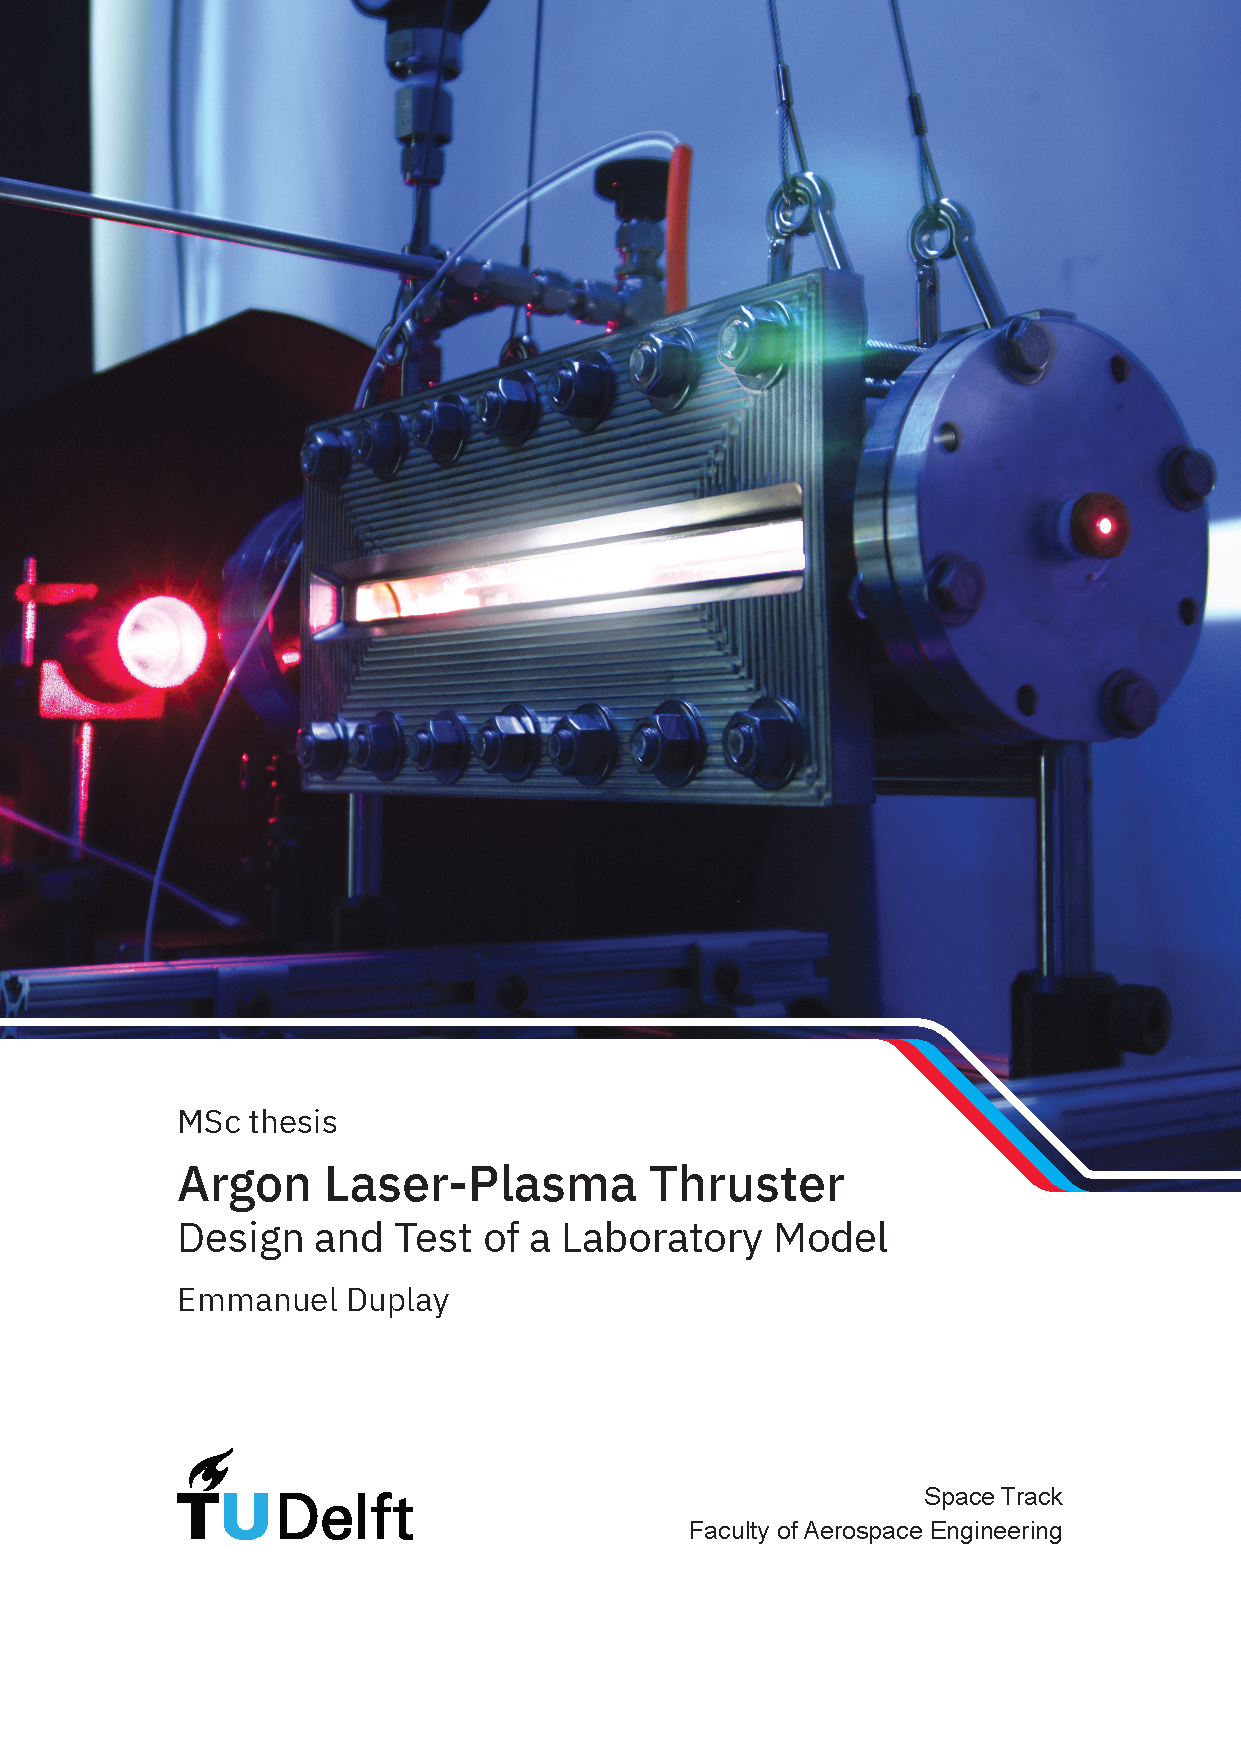
\includepdf{assets/cover.pdf}
    \begin{titlepage}
    \thispagestyle{empty}
    % \centering
    \sffamily
    \vspace*{3cm}
    {\large \color{cyan}
        % Suptitle
        Master's Thesis
    }

    \vspace{0.3cm}
    \textbf{{\LARGE Design and Test of an Argon Laser-Plasma Thruster\\Laboratory Model}}

    \vspace{0.2cm}
    {\large 
        % Subtitle
        Submitted to fulfill the requirements of the degree of Master of Science at\\the Delft University of Technology

        \vspace{1cm}
        Emmanuel Duplay \\
        5468515 \\
        MSc. Aerospace Engineering \\
        Space Track \\
        Space Exploration Profile

        \vspace{0.5cm}
        \today
    }
    \vfill
    {   
        The work in this thesis was performed in part at the Mechanical Engineering Department of McGill University, in Montreal, Canada.
        
        \setlength{\tabcolsep}{0pt}
        \begin{tabular}{l@{:\hspace{1em}}p{0.3\textwidth}p{0.4\textwidth}}
            Internal supervisor &   Ir. B.T.C. Zandbergen & Delft University of Technology \\
            External supervisor &   Prof. A.J. Higgins & McGill University \\
            % DON'T FORGET TO REPLACE THESE PLACEHOLDERS LMAO
            Thesis committee    &   S. Epstein, PE 
                        \newline    Dr. T.F. Shaw
                        \newline    Dr. W. Fujikawa
                                &   Masstech
                        \newline    UNSC Naval Research Laboratory
                        \newline    UNSC Naval Research Laboratory \\
        \end{tabular}
    }
    \vspace{0.5cm}
    \begin{center}
        
\includegraphics[height=1.75cm]{assets/TUDelft_logo.pdf}
        \hfill
        
\includegraphics[height=1.75cm]{assets/McGill_logo.pdf}
    \end{center}
    \pagenumbering{gobble}        
\end{titlepage}

    \newpage
    % \layout*
    {   \sffamily
        \thispagestyle{empty}
        \vspace*{\fill}
        % Text width: \the\textwidth  \\ % DELETE THIS LINE BEFORE SUBMITTING
        % Text height: \the\textheight  % DELETE THIS LINE BEFORE SUBMITTING

        The code used for this project (including the \LaTeX\hspace{0.67ex}source) is available on \\ \url{https://github.com/eeduplay/MScThesis} (latest) \\ \url{https://doi.org/10.1234/0000-00000-000} (archive)

        All experimental data associated with this thesis are available on \\
        \url{https://doi.org/10.1234/0000-00000-000}\\
        This includes the list of LSPs, high-speed footage, pressure data, and spectrograms.

        The author can be contacted by email at \href{mailto:emmanuel.duplay@gmail.com}{emmanuel.duplay@gmail.com}

        Cover image: Composite photograph approximating (with some artistic license) the appearance of the laser-thermal thruster model operating in the laboratory.
    }
    \pagenumbering{roman}

    % \newgeometry{left=4.2cm,right=4.2cm}
% \fancypagestyle{abstractplain}{
%     \fancyhf{}
%     \fancyfootoffset[lh]{0pt}
%     \fancyfoot[C]{\sffamily \thepage}  
% }
% \pagestyle{abstractplain}

% \phantomsection
% \begin{center}
%     \sffamily \Large \textbf{\caps{PREFACE}}
% \end{center}
%     \addcontentsline{toc}{chapter}{Preface}
%     \markboth{\MakeUppercase{Preface}}{}
%     \label{chp:preface}
%     \vspace{0.2cm}
%     This report documents the work done during my three month internship at the Princeton Plasma Physics Laboratory (PPPL). This project stems from a collaboration between McGill University and the PPPL, following the publication of \citetitle*{duplay_design_2022}, a mission design paper I worked on while finishing my undergraduate studies at McGill. This opportunity to collaborate arose about a month before the start of the summer, as I was still struggling to find an internship, so I would like to thank my former supervisor Andrew Higgins for arranging this experience. I would also like to thank Zhuofan Bao and Paria Makaremi-Esfarjani for their assistance with parts of this project. Finally, thanks to Ahmed Diallo, my supervisor at the PPPL, for inviting me to the PPPL and being a wonderful host.

% \restoregeometry
% \pagestyle{fancy}

\begin{plainchp}{Preface}
    \addcontentsline{toc}{chapter}{Preface}
    This report documents the work done during my three month internship at the Princeton Plasma Physics Laboratory (PPPL). This project stems from a collaboration between McGill University and the PPPL, following the publication of \citetitle*{duplay_design_2022}, a mission design paper I worked on while finishing my undergraduate studies at McGill. This opportunity to collaborate arose about a month before the start of the summer, as I was still struggling to find an internship, so I would like to thank my former supervisor Andrew Higgins for arranging this experience. I would also like to thank Zhuofan Bao and Paria Makaremi-Esfarjani for their assistance with parts of this project. Finally, thanks to Ahmed Diallo, my supervisor at the PPPL, for inviting me to the PPPL and being a wonderful host.
\end{plainchp}
    \hypersetup{linkcolor=black}
    \tableofcontents
    
    \listoffigures
    \addcontentsline{toc}{chapter}{List of Figures}
    
    \listoftables
    \addcontentsline{toc}{chapter}{List of Tables}
    \hypersetup{linkcolor=cyan}
    
    \chapter*{Nomenclature}
\setlength{\columnsep}{1cm}
\newenvironment{nomtable}
    {
        \centering
        \tabularx{\columnwidth}{r>{\raggedright\arraybackslash}X}
    }
    {
        \endtabularx
    }
\newenvironment{nomlist}
    {
        \begin{itemize}[leftmargin=1.5cm]
            \raggedright
            \setlength{\parsep}{0pt}
            \setlength{\itemsep}{-4pt}
    }
    {
        \end{itemize}
    }
\addcontentsline{toc}{chapter}{Nomenclature}
\markboth{\MakeUppercase{Nomenclature}}{}
\begin{multicols*}{2}
    % \setlength{\columnseprule}{1pt}
    \section*{Abbreviations}

    \begin{nomlist}
        \item[AEC   ] Atomic Energy Commission
        \item[AIAA  ] American Institute of Aeronautics and Astronautics
        \item[CFD   ] Computational Fluid Dynamics
        \item[CFL   ] Courant--Friedrichs--Lewy
        \item[DE    ] Directed-Energy 
        \item[DOE   ] (US) Department of Energy
        \item[FTCS  ] Forward Time Centered Space
        \item[HET   ] Hall-Effect Thruster
        \item[ITER  ] International Thermonuclear Experimental Reactor
        \item[LEP   ] Laser-Electric Propulsion
        \item[LSC   ] Laser-Supported Combustion
        \item[LSP   ] Laser-Sustained Plasma
        \item[LTP   ] Laser-Thermal Propulsion
        \item[NSTX] National Spherical Torus eXperiment
        \item[OOP] Object-Oriented Programming
        \item[OTV]  Orbital Transfer Vehicle 
        \item[PDE] Partial Differential Equation
        \item[PPPL  ] Princeton Plasma Physics Laboratory
        \item[SOR   ] Successive Over-Relaxation
        \item[TUD   ] Technische Universiteit Delft
    \end{nomlist}

    \section*{Latin symbols}
    \begin{nomlist}
        \item[$C$]             Courant number
        \item[$c_p$]           Specific heat of enthalpy
        \item[$D$]             Diameter
        \item[$d$]             Distance
        \item[$g_0$]           Standard gravity (9.80665~\unit{m/s^2}) 
        \item[$h$          ]   Enthalpy
        \item[$I$          ]   Local laser flux [W/m$^2$]
        \item[$I_\text{sp}$]   Specific impulse [s]
        \item[$k_L$        ]   Radiation absorption factor [1/m]
        \item[$m$]             Mass
        \item[$\mathcal{M}$]   Molar mass
        \item[$p$          ]   Pressure
        \item[$R$]             Gas constant
        \item[$r$          ]   Radial coordinate
        \item[$T$          ]   Temperature
        \item[$t$          ]   Time
        \item[$u$          ]   Axial velocity
        \item[$v$]             Velocity 
        \item[$z$          ]   Axial coordinate
    \end{nomlist}

    \section*{Greek symbols}
    \begin{nomlist}
        \item[$\alpha$]    Ionization mole fraction
        \item[$\beta$]     Dissociation mole fraction
        \item[$\theta$]    Azimuthal coordinate
        \item[$\kappa$]    Conductivity
        \item[$\lambda$]   Wavelength
        \item[$\rho$  ]    Density
        \item[$\phi$  ]    Radiation emission [W/m$^3$]
    \end{nomlist}

    \section*{Subscripts}
    \begin{nomlist}
        \item[c]   Thrust chamber
        \item[e]   Laser emitter
        \item[ex]  Exhaust
        \item[f]   Focusing length
        \item[g]   Specific (gas constant)
        \item[$i$] index along $x$ or $z$
        \item[$j$] index along $y$ or $r$
        \item[r]   Laser receiver
        \item[u]   Universal (gas constant)
    \end{nomlist}

    % \section*{Superscripts}
    % \begin{nomlist}
    %     \item[$n$]  time index
    % \end{nomlist}

\end{multicols*}

    \newpage
    \begin{plainchp}{Executive Summary}
    \addcontentsline{toc}{chapter}{Executive Summary}

    \lipsum[2-5]

\end{plainchp}

    \newpage
    \pagenumbering{arabic}

    % \chapter*{Unnumbered Chapter}
% \addcontentsline{toc}{chapter}{Unnumbered Chapter}  % Uncomment to include in ToC
% \markboth{\MakeUppercase{Unnumbered Chapter}}{}
    \chapter{Introduction} \label{chp:intro}
    
    \section{Motivation}

        In 2016, the Breakthrough Starshot initiative was proposed based on the work of \textcite{lubinRoadmapInterstellarFlight2016}. This mission involves sending \qty{1}{g} space probes to Alpha Centauri at \qty{20}{\%} the speed of light, using massive ground-based laser arrays. This could be enabled by a Moore's law in fiber laser technology, with a rapid doubling of power and a similar exponential decrease in costs. 
        
        As a near-term stepping stone using a smaller array, the laser can be coupled to a gas, reducing efficiency but increasing thrust. This process, Laser-Thermal Propulsion (LTP), would allow rapid interplanetary transfers, notably to Mars. The concept of LTP was first suggested by \textcite{kantrowitzRelevanceSpace1971} as a way to decrease launch costs and continues to be of interest. A conceptual design of an LTP spacecraft was proposed by \textcite{duplayDesignRapidTransit2022a}, with a similar architecture to Breakthrough Starshot: a \qty{10}{m} laser array beams \qty{100}{MW} of power to an orbiting spacecraft for injection burns. With a \qty{1}{ton} payload, \qty{6}{kN} of thrust and \qty{3000}{s} of $I_\mathrm{sp}$, a \qty{1}{h} laser beaming maneuver gives \qty{14}{km/s} of delta-V to the spacecraft, which reaches Mars in 45 days.

        \begin{figure}[!ht]
            \centering
            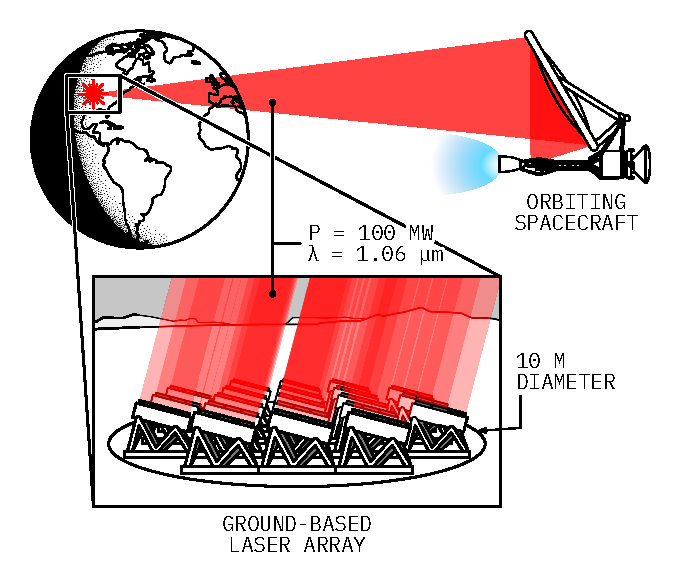
\includegraphics[width=0.4\textwidth]{assets/2 background/ltp_architecture.pdf}
            \caption{LTP architecture (\textcite{duplayArgonLaserPlasmaThruster2024a})}
            \label{fig:LTP architecture}
        \end{figure}

        In the thrust chamber of the vehicle, hydrogen is introduced. The laser is focused inside the chamber and is absorbed by the gas via inverse Bremsstrahlung, creating a Laser-Supported Plasma (LSP) core. Colder hydrogen flows around the LSP core and is heated by it to \qty{10000}{K}. The hot gas is then exhausted though a conventional converging-diverging nozzle at the exhaust velocity, imparting thrust to the vehicle.

        \begin{figure}[!ht]
            \centering
            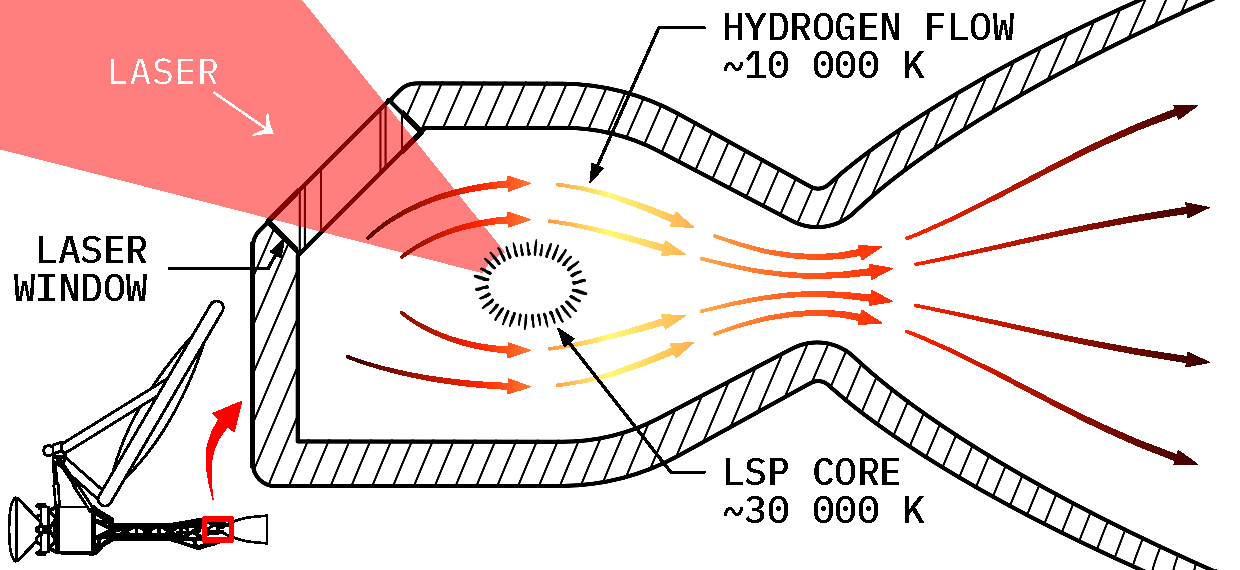
\includegraphics[width=0.6\textwidth]{assets/2 background/chamber.pdf}
            \caption{Overview of LTP system (\textcite{duplayArgonLaserPlasmaThruster2024a})}
            \label{fig:LTP system overview}
        \end{figure}

        In a conventional chemical rocket engine, the energy source is the oxidizer and the fuel, which are reacted together to release energy. They are transported with the rocket and set the temperature of the combustion reaction (typically \qtyrange{2000}{3000}{K}), which is directly related to the exhaust velocity.
        
        Separating the power source used for propulsion (here, the laser) from the spacecraft itself allows crucial weight savings, either increasing the payload mass fraction or decreasing transit time. Using a laser also allows for much greater thrust chamber temperatures than chemical propulsion, as the temperature of these plasmas is typically \qtyrange{15000}{30000}{K}. This gives in turn greater exhaust velocities. This propulsion method could therefore be an order of magnitude more efficient than our current rocket engines if certain engineering problems can be solved.

        Increasing the amount of energy deposited by the laser into the working gas remains a topic of active research and is a significant hurdle for the operational use of LTP. The two main conversion efficiencies are:
        \begin{enumerate}
            \item Absorption of the laser energy by the plasma
            \item Heat transfer from the plasma to the working gas (e.g. propellant)
        \end{enumerate}
        A selection of past LSP experiments will now be presented, with an emphasis on these efficiencies. As the efficiencies chosen are different from source to source, these will be defined where applicable.
    
    \section{Literature review}

        %Russian work: 1960s-2000s?

        The experimental basis of LTP was developed by \textcite{generalovContinuousOpticalDischarge1970} in 1970. For the first time, an LSP was generated with a \qty{150}{W} \ce{CO2} laser operating at \qty{10.6}{μm} wavelength. In this case, the LSP was initiated by a second, \qty{10}{kW} pulsed \ce{CO2} laser.
        
        %American work: 1970s-1990s?

        Work was done in the mid-1970s by \textcite{shojiLaserheatedRocketThruster1977,shojiPerformanceHeatTransfer1976a} to design a small-scale \qty{10}{kW} and full-scale \qty{5000}{kW} LTP engine. Carbon-seeded hydrogen was chosen to capture the plasma's radiation, which was mostly in the UV wavelength. \qty{20}{\%} of the laser power would be lost by convection and radiation to the walls in the \qty{10}{kW} thruster, with an additional \qty{5}{\%} of laser power lost by radiation through the thruster window. However, this was not tested. The \qty{10}{kW} prototype (\autoref{fig:Shoji apparatus}) was built and delivered to NASA at the conclusion of their effort.
        \begin{figure}[!ht]
            \centering
            \begin{subfigure}[t]{0.45\textwidth}
                \centering
                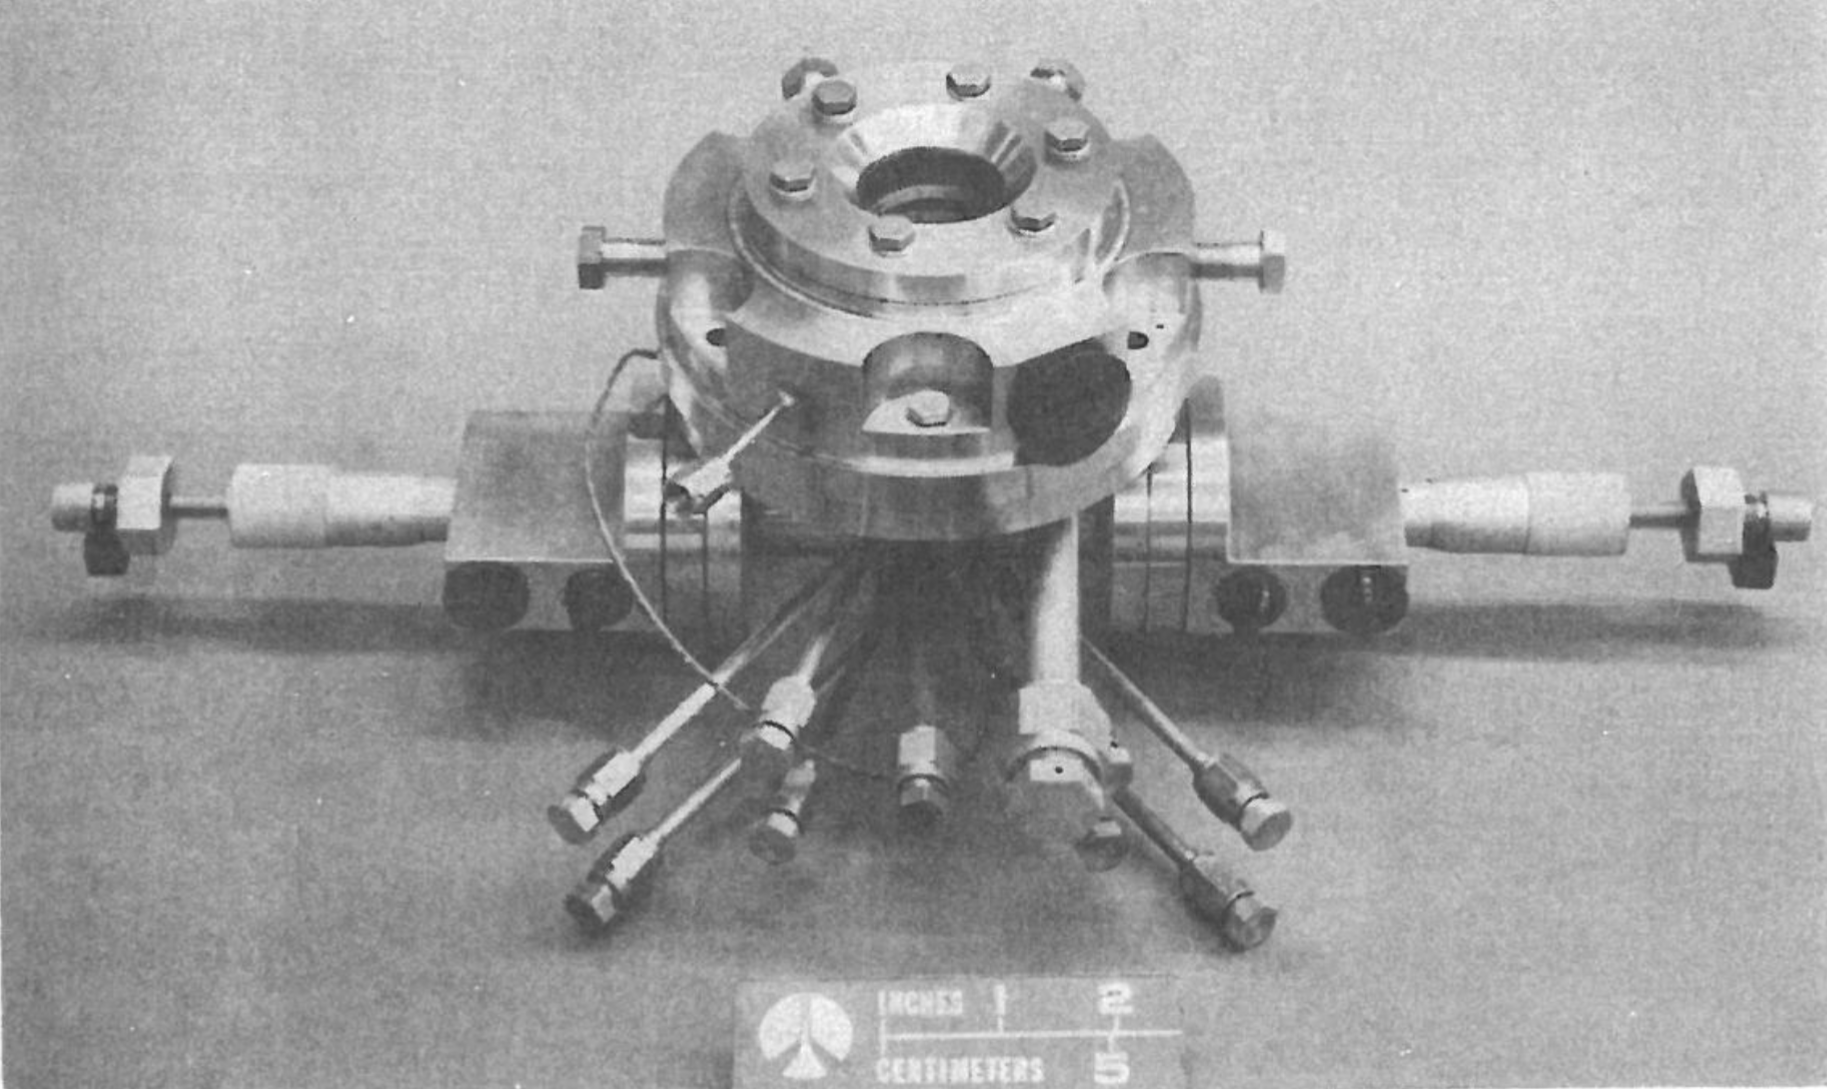
\includegraphics[width=\textwidth]{assets/2 background/Shoji_assy.png}
                \caption{\qty{10}{kW} thruster from \textcite{shojiPerformanceHeatTransfer1976a}}
                \label{fig:Shoji apparatus}
                \end{subfigure}
            \hfill
            \begin{subfigure}[t]{0.45\textwidth}
                \centering
                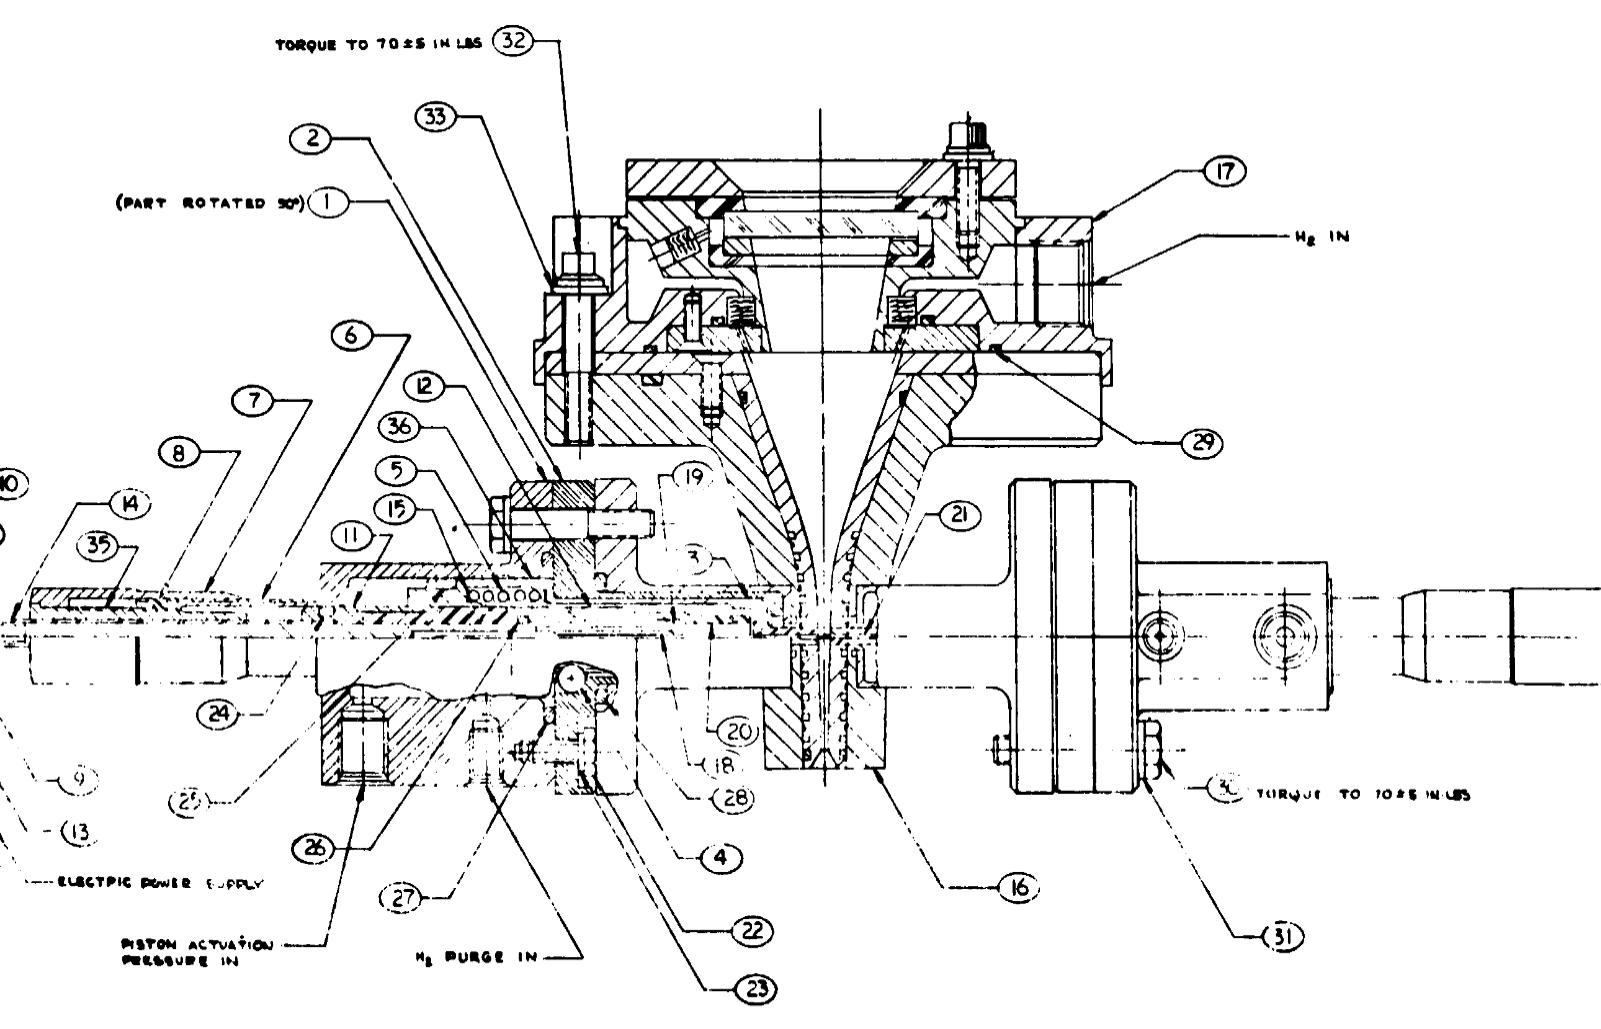
\includegraphics[width=\textwidth]{assets/2 background/Shoji cross-section.png}
                \caption{Cross-section drawing of \qty{10}{kW} thruster from \textcite{shojiLaserheatedRocketThruster1977} (original is of poor quality)}
                \label{fig:Shoji cross-section}
            \end{subfigure}
            \caption{Thruster designed by \textcite{shojiLaserheatedRocketThruster1977}}
            \label{fig:Shoji apparatussies}
        \end{figure}

        In the 1980s, \textcite{keeferPowerAbsorptionLasersustained1986a} studied LSP in a forced convective flow environment. Using a \qty{1.5}{kW} \ce{CO2} laser with power levels of \qtyrange{360}{840}{W} and pressures of \qtyrange{1.3}{2.3}{atm}, with varying argon flow velocities, the temperature field of the plasma was measured. From the temperature field, and assuming local thermodynamic equilibrium, the power absorbed by the plasma and the power radiated from it can be calculated.
        \begin{figure}[!ht]
            \centering
            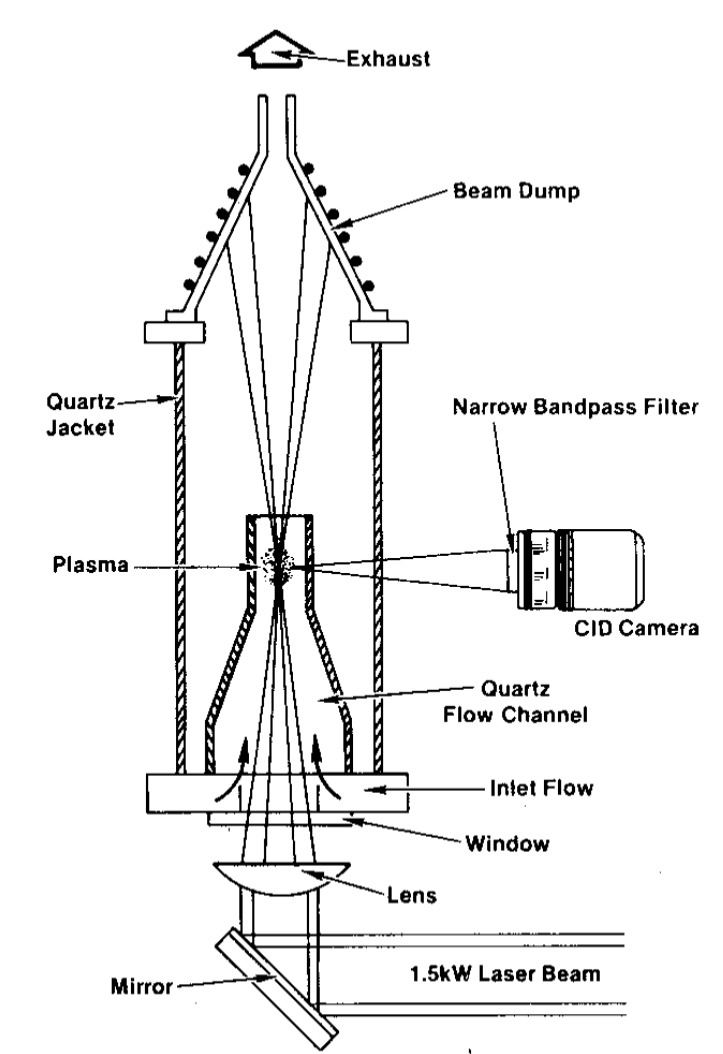
\includegraphics[width=0.4\textwidth]{assets/2 background/UTSI (Keefer) Apparatus.png}
            \caption{Experimental apparatus from \textcite{keeferPowerAbsorptionLasersustained1986a}}
            \label{fig:Keefer apparatus}
        \end{figure}
        \autoref{fig:Keefer apparatus} shows the apparatus used for these measurements. An inner quartz flow channel contained the plasma, while an outer quartz jacket contained the pressure. The plasma was initiated by laser heating of a tungsten rod, which was removed after initiation. Downstream, a water-cooled copper beam dump absorbed the energy of the laser and the heated argon flow, but was not used for measurements. The plasma's temperature was obtained through analyzing digital images. This temperature field was then used to calculate the power absorption and the radiation loss. The power absorbed by the plasma was between \qtyrange{23}{61}{\%} of incident laser power, while radiation loss was between \qtyrange{51}{80}{\%} of the absorbed power.

        Contemporary to \textcite{keeferPowerAbsorptionLasersustained1986a}, Mazumder and Krier headed a group at the University of Illinois that advanced the field of LTP. \textcite{krierContinuousWaveLaser1986a} reported laser absorption in an argon plasma approaching \qty{80}{\%}. \autoref{fig:Krier apparatus} shows the apparatus that was used by \textcite{krierContinuousWaveLaser1986a}, \textcite{zerkleLasersustainedArgonPlasmas1990} and \textcite{chenEmissionSpectroscopyCw1989a}. This vertical cylindrical flow chamber was made of 304 steel and had an internal diameter of 5 inches. A water-cooled calorimeter was used as a beam dump for the \qty{10}{kW} \ce{CO_2} laser. The laser energy not collected by the beam dump was assumed to be absorbed by the plasma, as the radiation reflected off the plasma is less than \qty{2}{\%} at these electron number densities. Moveable thermocouples gave two-dimensional maps of the flow surrounding the plasma core. The direct laser heating of the thermocouples and their carriage was taken into account.
        \begin{figure}[!ht]
            \centering
            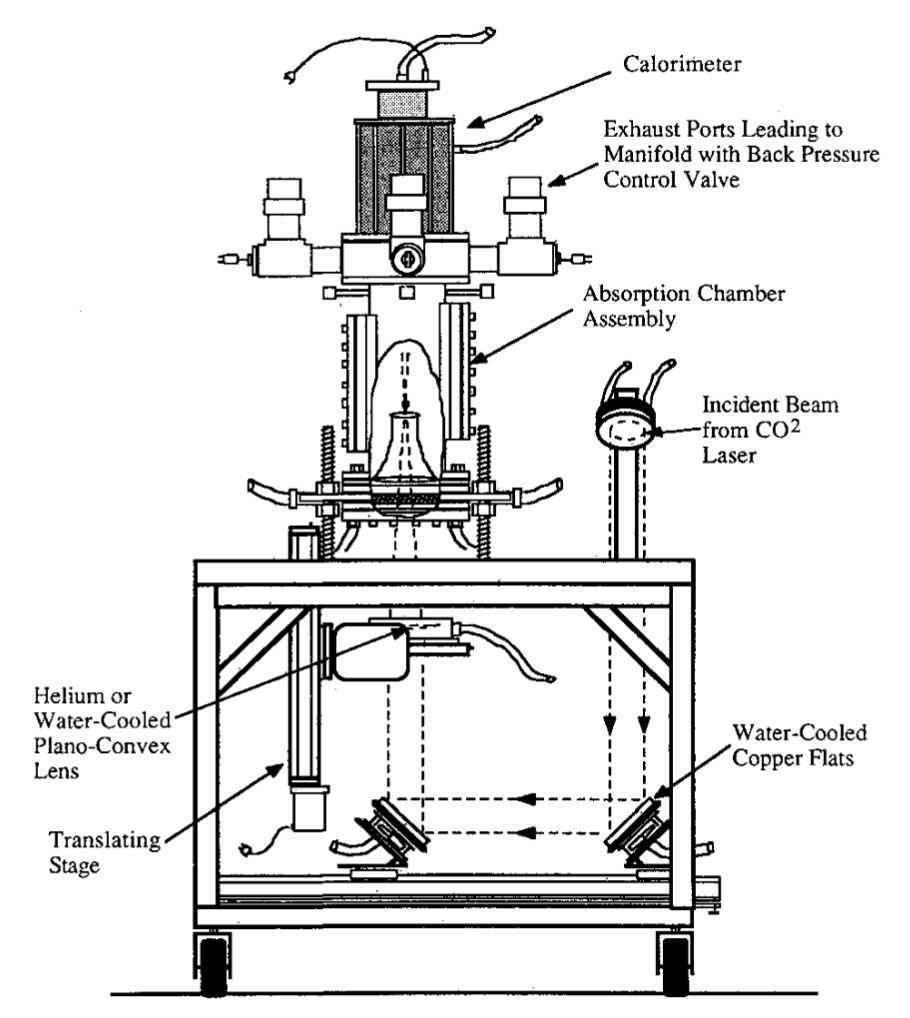
\includegraphics[width=0.5\textwidth]{assets/2 background/Illinois (Krier) Apparatus.png}
            \caption{Experimental apparatus from \textcite{zerkleLasersustainedArgonPlasmas1990}}
            \label{fig:Krier apparatus}
        \end{figure}
        These two-dimensional temperature maps \todo{INSERT EXPLANATION HERE}. Thermal efficiency was between \qtyrange{6}{25}{\%}, with radiative losses of \qty{64}{\%} and \qty{30}{\%}, 
        respectively. Thermal efficiency was defined as:


        \[\eta_\mathrm{th} =  \frac{\text{Power retained by the gas}}{\text{Incident laser power}}\]
        The minimum maintenance intensity of the plasma was also estimated at \qtyrange{0.1}{0.3}{MW/cm^2}.

        Further work by \textcite{zerkleLasersustainedArgonPlasmas1990} with the apparatus shown in \autoref{fig:Krier apparatus} reported absorption from \qtyrange{55}{97}{\%} and thermal efficiency from \qtyrange{11}{46}{\%}. This was done in \qtylist{1 2.5}{atm} of flowing argon, with laser powers up to \qty{7}{kW}. \textcite{chenEmissionSpectroscopyCw1989a} again increased the thermal efficiency of this apparatus, with \qtyrange{41}{62}{\%} of the laser energy being retained by the gas as thermal energy. This was among the highest thermal efficiencies measured by an LSP experiment. Here, \qty{86}{\%} of the laser's energy is absorbed by the LSP. This was attained with a \qty{5}{kW} \ce{CO2} laser, with flow speeds between \qtyrange{2}{10}{m/s}. They discuss that greater thermal efficiency is due to greater laser power, a high enough flow speed and a greater laser focusing $f$ number.

        Based on work by the Illinois group, an LTP engine demonstrator was tested in 1995 by \textcite{blackLaserPropulsion10kW1995} with a \qty{10}{kW} \ce{CO2} laser. This was planned to be a step towards a full-scale thruster. More than 100 thruster firings were completed, lasting 1 to 2 minutes each. The \qty{10}{kW} thruster is presented in \autoref{fig:Black apparatus}. It is mounted in a vacuum chamber to a thrust measurement assembly. Efficiency was calculated from:
        \[ \eta = \frac{F^2}{2 \dot{m} P_\mathrm{L}} \]
        with $P_\mathrm{L}$ the input laser power at the thruster window. Both argon and hydrogen were used. Argon propellant produced \qty{200}{s} of $I_\mathrm{sp}$ and a peak efficiency of 0.24. With hydrogen propellant, an $I_\mathrm{sp}$ of \qty{350}{s} and a peak efficiency of 0.37 were reported.
        \begin{figure}[!ht]
            \centering
            \begin{subfigure}[t]{0.3\textwidth}
                \centering
                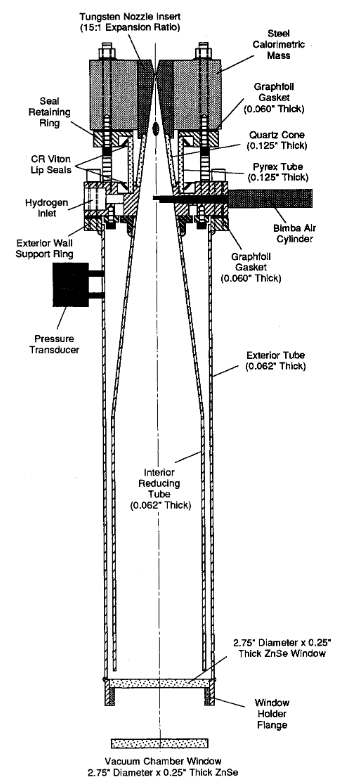
\includegraphics[width=\textwidth]{assets/2 background/BlackKrier thruster.png}
                \caption{\qty{10}{kW} thruster}
                \label{fig:Black apparatus}
            \end{subfigure}
            \hfill
            \begin{subfigure}[t]{0.45\textwidth}
                \centering
                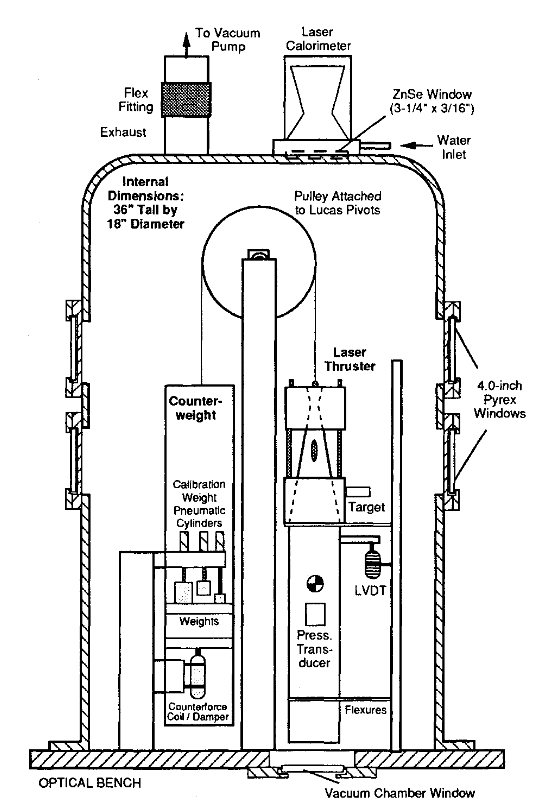
\includegraphics[width=\textwidth]{assets/2 background/Black thrust measurement assy.png}
                \caption{Thrust measurement assembly}
                \label{fig:Black thrust measurement}
            \end{subfigure}
            \caption{Apparatus used in \textcite{blackLaserPropulsion10kW1995}}
            \label{fig:Black apparatussies}
        \end{figure}
        A preliminary design for the full-scale \qty{100}{kW} thruster was also presented, with a predicted specific impulse of \qty{1000}{s}, thrust of \qty{4.5}{N} and a conversion efficiency of \qty{80}{\%}.

        %Chinese and Japanese work: 1980s-2020s

        In the early 2000s, \textcite{toyodaThrustPerformanceCW2002} built and tested two different thruster models, presented in \autoref{fig:Toyoda apparatussies}. These thrusters, using argon or nitrogen heated by LSP, were powered by a \qty{2}{kW} \ce{CO2} laser. The LSPs were initiated by a retractable tungsten rod at the laser's focus. Thrust measurements were done both in atmospheric pressure and in vacuum. This comparative study showed that confining the plasma into a smaller chamber increased heat transfer and therefore, efficiency. \textcite{toyodaThrustPerformanceCW2002} defined the energy conversion efficiency as the amount of laser power that is converted into usable kinetic energy for thrust. It is calculated as\footnote{As mentioned by \textcite{duplayArgonLaserPlasmaThruster2024a}, there appears to be a typographical error in the reference as the units are inconsistent. The corrected equation is presented here.}:
        \[ \eta_\mathrm{e} =  \frac{F^2_\mathrm{hot} -F^2_\mathrm{cold}}{2 \dot{m} P}\]
        Where $F_\mathrm{hot}$ is the thrust with laser on, $F_\mathrm{cold}$ is the cold flow thrust (laser off) and $P$ is incident laser power. An energy conversion efficiency of 37\% and an $I_\mathrm{sp}$ of \qty{113}{s} were measured with the second model \autoref{fig:Toyoda apparatus 2} in vacuum with argon propellant. The pressure ratio, defined as the chamber pressure divided by the nozzle exit pressure, was 420. A water cooling system measured the heat loss to the walls to be 55\% of incident laser power, with a final 8\% being ``other loss". Heat loss to the walls was expected to be recycled with regenerative cooling in a real-world application.

        \begin{figure}[!ht]
            \centering
            \begin{subfigure}[t]{0.45\textwidth}
                \centering
                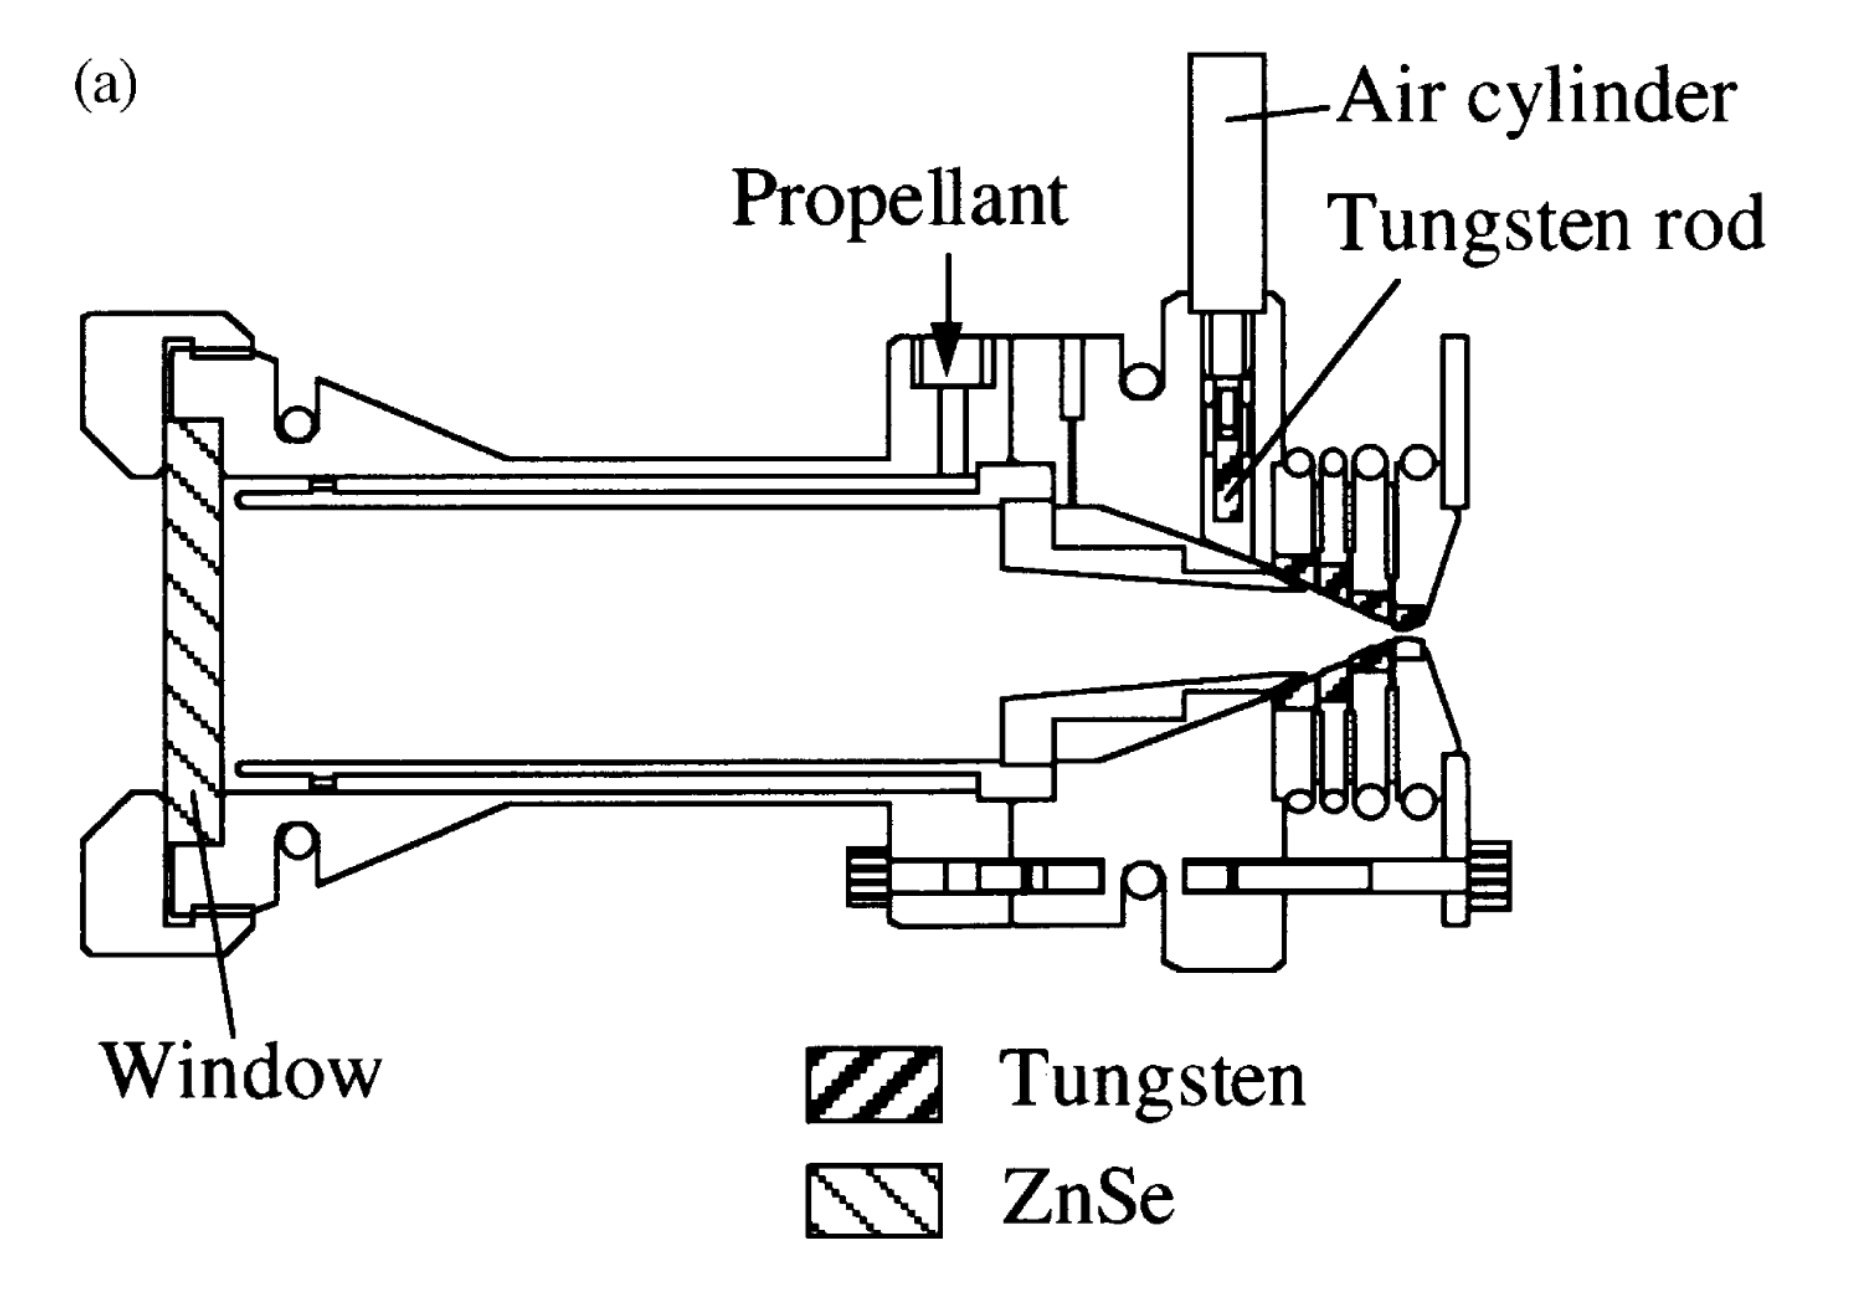
\includegraphics[width=\textwidth]{assets/2 background/Toyoda apparatus model 1.jpg}
                \caption{Model I}
                \label{fig:Toyoda apparatus 1}
            \end{subfigure}
            \hfill
            \begin{subfigure}[t]{0.45\textwidth}
                \centering
                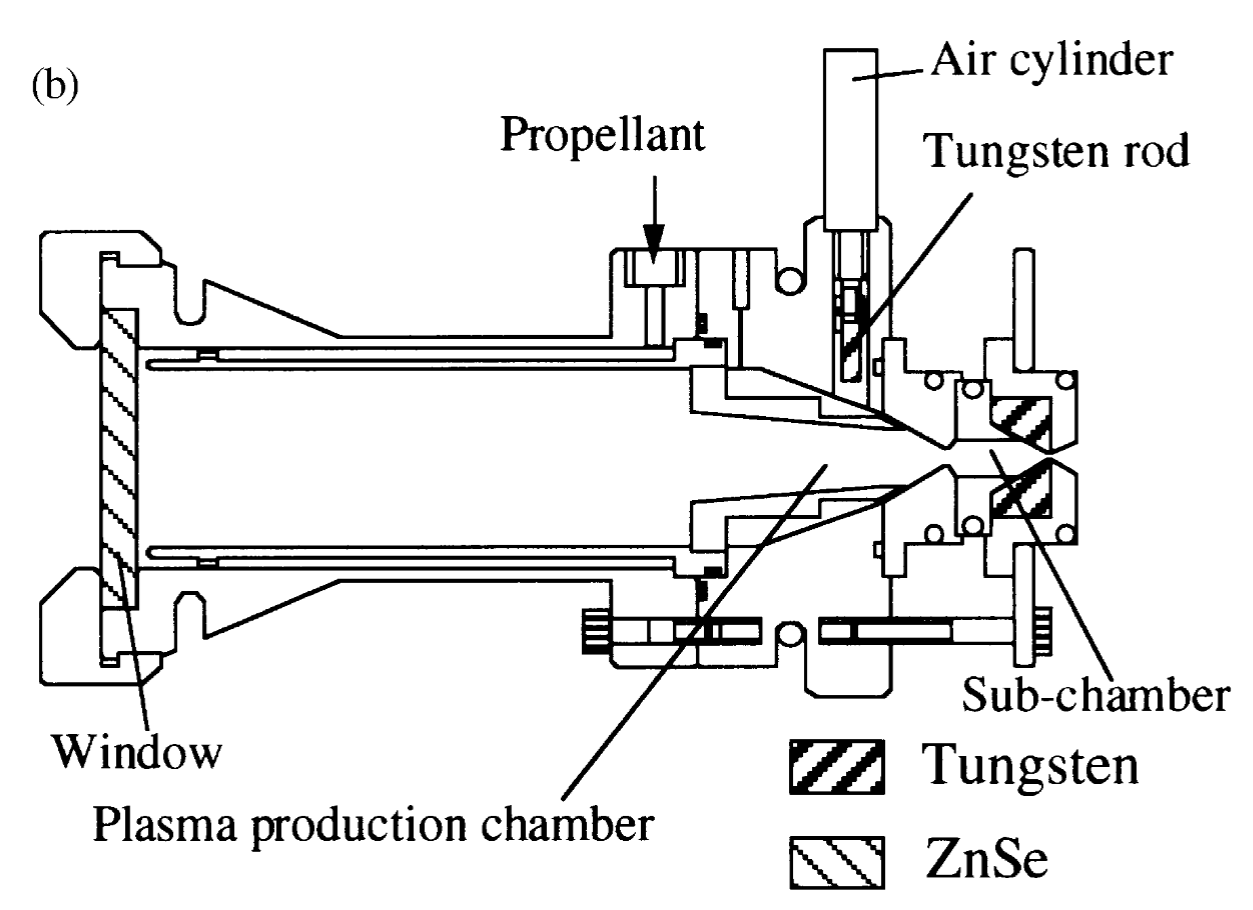
\includegraphics[width=\textwidth]{assets/2 background/Toyoda Apparatus model 2.png}
                \caption{Model II}
                \label{fig:Toyoda apparatus 2}
            \end{subfigure}
            \caption{Two thruster models from \textcite{toyodaThrustPerformanceCW2002}}
            \label{fig:Toyoda apparatussies}
        \end{figure}

        \textcite{luCharacteristicDiagnosticsLaserStabilized2022a} investigated LSP for lighting applications instead of propulsion. Therefore, an emphasis was made on spectroscopy measurements. A \qty{300}{W} fiber laser at a wavelength of \qty{1080}{nm} was focused to a \qty{50}{μm} diameter spot in a high pressure chamber.
        \begin{figure}[!ht]
            \centering
            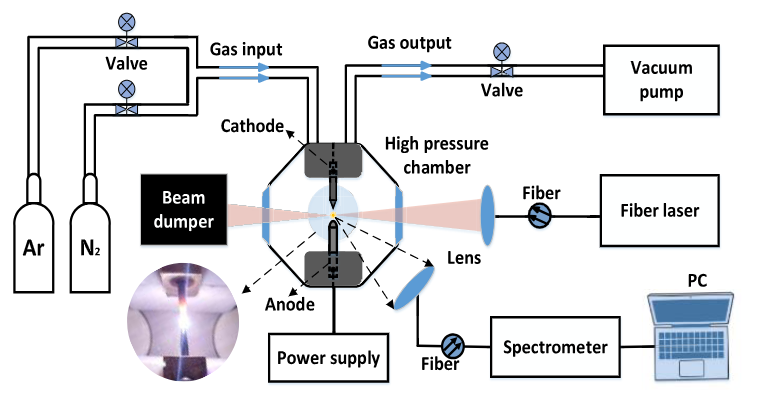
\includegraphics[width=0.7\textwidth]{assets/2 background/Lu apparatus.png}
            \caption{Experimental setup from \textcite{luCharacteristicDiagnosticsLaserStabilized2022a}}
            \label{fig:Lu apparatus}
        \end{figure}
        Argon was used, with pressures between \qtyrange{10}{20}{bar}. A lower initiation power (\qty{117}{W}) than other studies was achieved at \qty{20}{bar}. This was attributed to the smaller focus delivering a greater photon flux. \ce{N2} was later added between \qtyrange{0.1}{1.0}{\%}. As expected, increasing the laser power or the gas pressure was found to increase the radiation intensity of the LSP. However, adding \ce{N2} reduced both the electron temperature and electron density of the LSP, reducing its radiation intensity.

        Seeding the working gas with another species has been discussed as a way to increase the energy absorption into the working fluid of an LTP engine. LSPs in pure methane and methane-seeded gasses have been investigated by \textcite{kameiMethaneMethaneXenon2020}. Methane dissociates into hydrogen and carbon with the high temperature of the LSP. As mentioned with \textcite{shojiLaserheatedRocketThruster1977}, carbon particles would absorb the LSP's UV radiation.  A \qty{1.1}{kW} diode laser at a wavelength of \qty{940}{nm} was beamed into a high-pressure chamber fitted with arc initiation electrodes. The gap between these electrodes was \qty{1}{mm}. A CCD type spectrometer recorded emission spectra of the initiation arc discharge and of the LSP. LSPs in three different gasses were attempted: pure methane, methane-argon, and methane-xenon.
        
        In methane at \qty{0.1}{MPa}, soot formation between the electrodes prevented LSP initiation. The spectrometer confirmed the dissociation of methane, as line spectra of carbon and hydrogen were observed at the initiation arc. Initiation was also unsuccessful in argon-methane with a pressure between \qtyrange{0.1}{0.3}{MPa} and a methane volume fraction between \qtyrange{20}{60}{\%}. LSP was successfully generated in methane-xenon, with a lower threshold power (\qty{850}{W}) than in pure xenon. The partial pressure of methane was between \qtyrange{0.02}{0.6}{MPa}, with a partial pressure of xenon of \qty{0.10}{MPa}.

        \textcite{takanoDemonstrationDiodeLasersustained} used a diode laser emitting simultaneously at \qty{927}{nm} and \qty{951}{nm} to generate LSPs in argon. This resulted in an $I_\mathrm{sp}$ of \qty{105}{s} and a thrust efficiency of \qty{8}{\%}. This $I_\mathrm{sp}$ was calculated from the plenum pressure when the laser was on. They define thrust efficiency as:
        \[
        \eta = \frac{g_0 I_\mathrm{sp} (F_\mathrm{hot}-F_\mathrm{cold})}{2 P_\mathrm{laser}}
        \]
        Two setups were used: the LSP generation chamber previously used by \textcite{kameiMethaneMethaneXenon2020} (\autoref{fig:Takano LSP generation chamber}) and an LSP thruster (\autoref{fig:Takano LSP thruster}).
        \begin{figure}[!ht]
            \centering
            \begin{subfigure}[t]{0.45\textwidth}
                \centering
                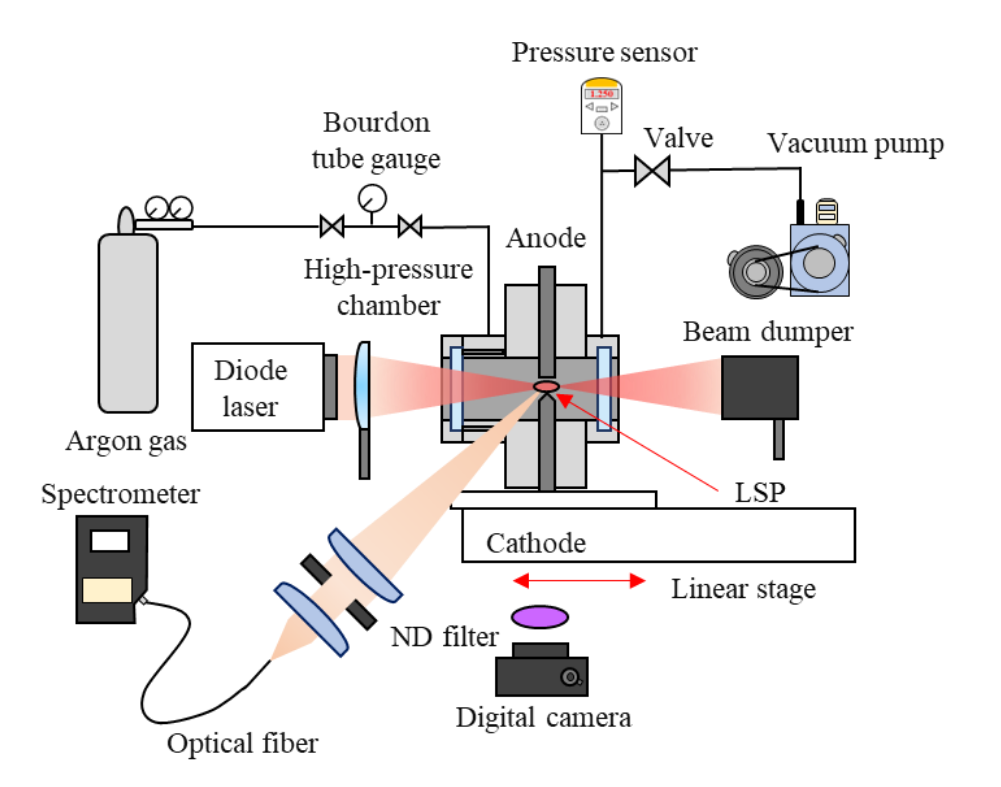
\includegraphics[width=\textwidth]{assets/2 background/Takano LSP chamber.png}
                \caption{LSP generation chamber and systems}
                \label{fig:Takano LSP generation chamber}
            \end{subfigure}
            \hfill
            \begin{subfigure}[t]{0.45\textwidth}
                \centering
                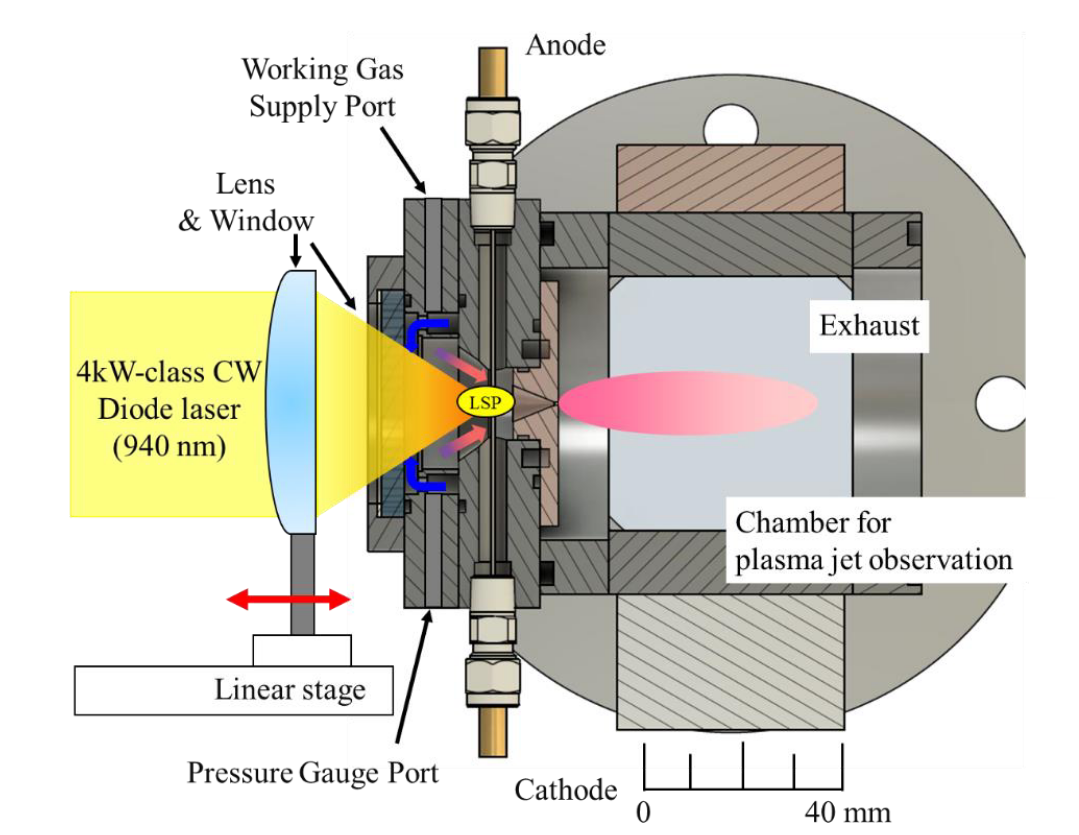
\includegraphics[width=\textwidth]{assets/2 background/Takano LSP thruster.png}
                \caption{LSP thruster}
                \label{fig:Takano LSP thruster}
            \end{subfigure}
            \caption{LSP setups from \textcite{takanoDemonstrationDiodeLasersustained}}
            \label{fig:Takano apparatussies}
        \end{figure}
        The LSP chamber was used to determine the effect of various F-numbers on the argon LSP. The thruster has an interchangeable copper throat, with diameters of \qty{0.7}{mm} and \qty{1.0}{mm}. In both setups, electric arc initiation was used. Once initiated in the thruster, the LSP is moved toward the nozzle with the lens mounted on a motorized stage. It was found that moving the LSP this way increased the heat exchange with the working gas. Thrust was calculated by using the pressure measurements inside the thruster's heating chamber.

        %Canadian work: 2020s  

        \textcite{duplayArgonLaserPlasmaThruster2024a} used a \qty{3}{kW} pulsed fiber laser to create LSPs in static and flowing argon. In static argon, about \qty{80}{\%} of the laser energy was being absorbed by the plasma, with approximately \qty{15}{\%} of the laser energy heating the bulk gas. This was done between \qtyrange{5}{20}{bar}.
        \begin{figure}[!ht]
            \centering
            \includegraphics[width=0.7\textwidth]{assets/2 background/finalsetup_static.pdf}
            \caption{Static LSP apparatus from \textcite{duplayArgonLaserPlasmaThruster2024a}}
            \label{fig:Duplay apparatus}
        \end{figure}

    \section{Summary and direction of work in this thesis}
        
        From the literature review, \autoref{tab:lit review summary} and \autoref{tab:efficiencies} were compiled. Most studies have used \ce{CO2} lasers with a wavelength of \qty{10.6}{μm}. Use of a \ce{CO2} laser for power beaming to a remote target for propulsion applications is limited by the range over which the laser can be focused due to their long laser wavelength. 
    
        Indeed, the diffraction limit of a laser, which is the theoretical lower limit on beam divergence, equals the wavelength ($\lambda$) divided by the diameter $D$ of the output beam \cite{hechtUnderstandingLasersEntry2019}.
        \[
        \text{Diffraction limit (radians)} = \lambda/D
        \]
        This relegated \ce{CO2} lasers to ground-to-orbit launch. Recently, high power fiber lasers emitting near \qty{1}{μm} have become readily available. Being able to beam energy to low earth orbit, fiber lasers make laser propulsion more feasible.

        \begin{table}[!ht]
            \centering
            \caption{Summary of a selection of past LSP experiments. $\lambda$: wavelength, $P$: maximum laser power, $p$: pressure, $\dot m$: mass flow rate, $I_\mathrm{sp}$: maximum specific impulse, $F_\mathrm{T}$: maximum thrust}
            \label{tab:lit review summary}
            \begin{tabularx}{\textwidth}{@{}>{\small}X<{\raggedright}lXXrXXXrr<{\raggedright}@{}}
            \toprule
            {\normalsize LSP   Facility} & Year & Laser & $\lambda$ [\unit{\um}] & $P$ [kW] & Gas & $p$ [atm] & $\dot m$ [g/s] & $I_\mathrm{sp}$ [s] & $F_\mathrm{T}$ [N]  \\ \midrule
            \textcite{generalovContinuousOpticalDischarge1970}        &1970&\ce{CO_2}&10.60&0.15 &\ce{Xe}           & 3.0-4.0  &  -  & -   &  -   \\
            \textcite{keeferPowerAbsorptionLasersustained1986a}       &1986&\ce{CO_2}&10.60&0.84 &\ce{Ar}           & 1.3-2.3  & 0.01-0.19   & -   &  -   \\
            \textcite{krierContinuousWaveLaser1986a}                  &1986&\ce{CO_2}&10.60&10  &\ce{Ar}           &     -       & 2.3-4.6 & -& -\\
            \textcite{zerkleLasersustainedArgonPlasmas1990}           &1988&\ce{CO_2}&10.60&7   &\ce{Ar}           &      -      &     -     & -&- \\
            \textcite{chenEmissionSpectroscopyCw1989a}                &1989&\ce{CO_2}&10.60&5   &\ce{Ar}           &      -      &  -  & -   & -    \\
            \textcite{blackLaserPropulsion10kW1995}                   &1995&\ce{CO_2}&10.60&10  &\ce{Ar}           & 1.4-2.4  & 5.1-9.4 & 200 & 7 \\
                                                                      &    &\ce{CO_2}&10.60&10  &\ce{H_2}          &    3.4        & 1.1&  350   & 3 \\
            \textcite{toyodaThrustPerformanceCW2002}                  &2002&\ce{CO_2}&10.60&2   &\ce{Ar}, \ce{N_2} & 2.0-5.5  &  -  & 113 & 0.44 \\
            \textcite{luCharacteristicDiagnosticsLaserStabilized2022a}&2022&Fiber    &1.08 &0.30 &\ce{Ar}, \ce{N_2} & 9.9-19.7 &  -  & -   & -    \\ 
            \textcite{takanoDemonstrationDiodeLasersustained}         &2024&Diode    &0.927 and 0.951 &4.4 &\ce{Ar}   & 10-15 &   - & 105   & -    \\
            \textcite{duplayArgonLaserPlasmaThruster2024a}            &2024&Fiber    &1.07  & 3 &\ce{Ar}            &   5-20  & 0 & - & - \\
            \bottomrule
            \end{tabularx}
        \end{table}

        \begin{table}[!ht]
            \centering
            \caption{Comparative table of experimental LTP thruster efficiencies}
            \label{tab:efficiencies}
            \begin{tabularx}{\textwidth}{@{}>{\small}X<{\raggedright} r l r@{}}
            \toprule
            {\normalsize LSP   Facility}   & Laser absorption  & Efficiency & Value of efficiency \\ \midrule
            \textcite{keeferPowerAbsorptionLasersustained1986a}   & 0.23 - 0.61      &          -        &                 -          \\
            \textcite{krierContinuousWaveLaser1986a}       & 0.50 - 0.80         & $\eta_\mathrm{th} =  \frac{\text{Power retained by the gas}}{\text{Incident laser power}}$ &  0.06 - 0.25 \\
            \textcite{zerkleLasersustainedArgonPlasmas1990}       & 0.55 - 0.97   &         $\eta_\mathrm{th} =  \frac{\text{Power retained by the gas}}{\text{Incident laser power}}$ &  0.11 - 0.46 \\
            \textcite{chenEmissionSpectroscopyCw1989a}          & 0.86                      &  $\eta_\mathrm{th} =  \frac{\text{Power retained by the gas}}{\text{Incident laser power}}$  &  0.41-0.62  \\
            \textcite{blackLaserPropulsion10kW1995}       &  -  & $ \eta = \frac{F_\mathrm{hot}^2}{2 \dot{m} P_\mathrm{L}} $& 0.20 - 0.25 (Ar), 0.25 - 0.40 (H)     \\
            \textcite{toyodaThrustPerformanceCW2002}    & -                      & $ \eta_\mathrm{e} =  \frac{F^2_\mathrm{hot} -F^2_\mathrm{cold}}{2 \dot{m} P} $     &   0.37 \\
            \textcite{takanoDemonstrationDiodeLasersustained}  &       -       & $ \eta = \frac{g_0 I_\mathrm{sp} (F_\mathrm{hot}-F_\mathrm{cold})}{2 P_\mathrm{laser}} $ & 0.08 \\ 
            \textcite{duplayArgonLaserPlasmaThruster2024a}  &  0.80&  $\eta_\mathrm{th} =  \frac{\text{Power retained by the gas}}{\text{Incident laser power}}$ & 0.15 \\
            \bottomrule
            \end{tabularx}
        \end{table}
        

        To increase thermal efficiency, \textcite{chenEmissionSpectroscopyCw1989a} suggest:
        \begin{enumerate}
            \item A greater laser power, which gives greater inverse bremsstrahlung absorption coefficient and longer absorption path length;
            \item A high enough flow speed to push the LSP back to the laser focus, but not too fast as to blow the plasma out;
            \item A greater laser focusing $f$ number, creating a longer and narrower plasma. This increases the probability a photon will be absorbed by the plasma and reduces the radiation loss.
        \end{enumerate}

        For a small-scale demonstration thruster, $I_\mathrm{sp}$ values near \qty{100}{s} can be expected, with thrust values under \qty{1}{N}, as was found by \textcite{toyodaThrustPerformanceCW2002} and \textcite{takanoDemonstrationDiodeLasersustained}.

        % Previous objective: The objective of this research project will be to test a lab-scale proof-of-concept LTP thruster for interplanetary space flight, using a \qty{1.07}{μm} fiber laser. Key performance parameters of this thruster such as thrust and specific impulse will be measured, and the LSP heating core inside the thruster will be characterized. 
        
        
        The objective of this research project will be to test a lab-scale proof-of-concept LTP thruster for interplanetary space flight, using a \qty{1.07}{μm} fiber laser \todo{add to this}. This project will mainly build upon the experimental research started by \textcite{duplayArgonLaserPlasmaThruster2024a}.
        
        % Link to next chapter, modelling c_p
        Before going into experiments, it is important to characterize certain thermodynamic properties of the gasses used. Notably, the modelling of heat capacity will be presented in the next chapter.

    \chapter{Background} \label{chp:background}
    \section{Russian work: 1960s-2000s?}
    \section{American work: 1970s-1990s?}
    \section{Japanese work: 1980s-2020s?}
    \section{Chinese work: 2020s?}
    \section{Canadian work: 2020s}
    \section{Summary and direction of work in this thesis}

        \begin{table}[ht]
            \small
            \centering
            \caption{Summary of a selection of past LSP experiments. $\lambda$: wavelength, $P$: maximum laser power, $p$: pressure, $I_\mathrm{sp}$: maximum specific impulse, $F_\mathrm{T}$: maximum thrust}
            \label{tab:pastexp}
            \begin{tabularx}{\textwidth}{@{}>{\small}X<{\raggedright}llrrlrrr>{\footnotesize}X<{\raggedright}@{}}
            \toprule
            {LSP   Facility}                                                           & Year & Laser         & $\lambda$   [\unit{\um}] & $P$ [kW] & Gas                 & $p$   [atm] & $I_\mathrm{sp}$ [s] & $F_\mathrm{T}$   [N] & {Comments}                                                                   \\ \midrule
            \textcite{generalovContinuousOpticalDischarge1970}                                                         & 1970 & \ce{CO_2}                  & 10.60             & 0.15               & \ce{Xe}              & 3.0 - 4.0        &           -             &       -       & First   LSP                                                                \\
            \textcite{keeferPowerAbsorptionLasersustained1986}         & 1986 & \ce{CO_2}                  & 10.60             & 0.84        & \ce{Ar}              & 1.3   - 2.3      &            -            &       -       & Specialized   laser beam dump integrated within the converging exit nozzle \\
            \textcite{blackLaserPropulsion10kW1995}          & 1995 & \ce{CO_2}                  & 10.60             & 10.00              & \ce{Ar},   \ce{H_2}    & 1.0   - 2.7      & 350                    & 3.00         & 15:1   expansion ratio nozzle                                              \\
            \\
            \textcite{toyodaThrustPerformanceCW2002} & 2002 & \ce{CO_2}                  & 10.60             & 2.00               & \ce{Ar},   \ce{N_2}    & 2.0   - 5.5      & 113             & 0.44         & Tungsten   rod ignition                                                    \\
            \textcite{zimakovInteractionNearIRLaser2016}                                                        & 2016 & Fiber                & 1.07              & 1.50        & \ce{Ar},   \ce{Xe}   & 3.0   - 24.7     & -                      & -            & Arc   discharge ignition                                                   \\
            \textcite{matsuiGeneratingConditionsArgon2019}                                                          & 2019 & Fiber &      1.07             &        2.00            &           \ce{Ar}           &          1.0 - 64.2        &            -            &       -       & Arc   discharge ignition                                                   \\
            \textcite{luCharacteristicDiagnosticsLaserStabilized2022a}                                                             & 2022 & Fiber                & 1.08              & 0.30      & \ce{Ar},   \ce{Ar + N_2} & 9.9   - 19.7     & -                      & -            & Arc   discharge ignition                                                   \\ \bottomrule
            \end{tabularx}
        \end{table}

        The original contribution of this work 


        % Higgins text from email to Mark Wolverton: Laser thermal propulsion originated with Arthur Kantrowitz, who was involved in developing the first gas dynamic lasers that would be able to reach MW-class power in the 1960s. (Interesting connection to Jordin Kare: Jordin was also a filk-singer, which is a science-fiction themed version of folk singing. He actually wrote a song about laser thermal propulsion called “Kantrowitz 1972”. Put your coffee cup down before listening to this…) 
        %The laser-thermal rocket kind of died with the demise of high-power laser weapon research in the early 1990s. Now with Phil Lubin’s work, I think it is worthwhile looking at again. Even with a gigawatt-class laser, laser propulsion is not well suited for ground-to-orbit launch vehicles, unless they are very small (this is what Jordin’s filk song is about—rapid turn around of launching many microlaunchers using a laser).  Here’s the clip of Elon Musk making the same point: https://youtu.be/viRylmoFAj0?si=MzzsBkhHF71FLCRG
        %However, with Philip Lubin’s demonstration that phased array lasers can be made arbitrarily large, we can now reach much deeper into space and perform propulsive maneuvers more leisurely (say, over hours), so the power requirements now drop to the 100s of MW (rather than 10s of gigawatts!). This was the basis of our 45-days-to-Mars study, which I think you have already seen. Here is an un-paywalled version of it: [2201.00244] Design of a rapid transit to Mars mission using laser-thermal propulsion (arxiv.org)
        %The other approach is to provide laser power onto a solar panel (although one tuned to the laser wavelength) that then powers electric propulsion like an ion engine or Hall effect thruster: Laser-electric propulsion. Lubin’s group published a similar study to ours, trying to hit similar objectives (the usual “Mars in a month” metrics). I’ve attached their paper here: SheerinLubinEtAl_FastTransporationElectricPropulsionDirectedEnergy_ActaAstro2021
        %Their paper and ours make for a nice “compare and contrast” of the pluses and minuses of the laser-electric and laser-thermal approaches.

    \chapter{Facility design}

    \section{Version 1 test section} \label{sec:design_v1}

        The design process of the first generation thruster, called Version 1 (V1), can be found in \textcite{duplayArgonLaserPlasmaThruster2024a}. It proved to be a dependable prototype, repurposed from a previous unrelated experiment. However, it presented problems that required a second generation prototype to be designed and manufactured.

        \begin{figure}[!ht]
            \centering
            \begin{subfigure}[t]{\textwidth}
                \includegraphics[width=0.85\textwidth]{assets/3 design/finalsetup_static.pdf}
                \caption{Static setup}
            \end{subfigure}
            \hfill
            \begin{subfigure}[t]{\textwidth}
                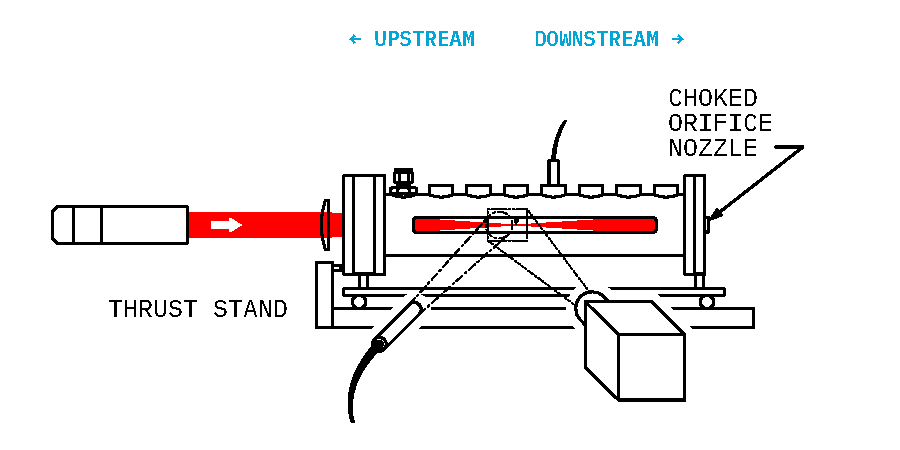
\includegraphics[width=0.85\textwidth]{assets/3 design/finalsetup_flowing.pdf}
                \caption{Flowing setup}
            \end{subfigure}
            \caption{V1 LTP thruster}
            \label{fig:V1 setup}
        \end{figure}

        298 recorded pulsed laser shots were conducted with V1, exploring the power-pressure threshold, wire initiation and spark initiation. A side window permitted direct visualization of the LSP with a high speed camera (Photron Fastcam SA5).

        % Adding holes on bottom for wire ignition

        However, this test section was made of steel, creating too much friction on its rails during thrust tests. This was mitigated in part by a rope system mentioned in \textcite{duplayArgonLaserPlasmaThruster2024a}, but was not found to be repeatable. Having the LSP heat a smaller internal volume than the \qty{0.4}{L} of V1 was also desirable, as a greater effect on internal pressure and thrust would be seen.

        Critically, rubber seals were exposed to the laser path during continuous (CW) lasing with a lower focal length lens (picture), severely burning them in the only CW test conducted. A shorter test section designed for a \qty{100}{mm} focal length lens would solve this.

    \section{Version 2} \label{sec:design_v2}

        To improve upon the V1 facility, an entire LTP thruster redesign was done. This resulted in the much smaller Version 2 (V2) purpose-built LTP thruster at the end of April 2024.

        \subsection{Requirements}

            The following requirements were developed for the design of the V2 thruster. The objective was to detect a measurable difference in thrust between an argon cold gas thruster and an argon “hot gas” thruster, heated by a laser supported plasma (LSP).

            \begin{enumerate}
                \item Laser thruster
                \begin{enumerate}
                    \item A \qty{300}{W} Continuous Wave (CW) \qty{1070}{nm} laser shall sustain the plasma (Nominal power \qty{300}{W}, actual max power \qty{350}{W})
                    \item The thruster shall have a minimum safe “hot” operation time of \qty{30}{s}
                    \begin{enumerate}
                        \item In the event of failed LSP initiation, the thruster shall safely absorb the total laser power for at least \qty{10}{s}
                    \end{enumerate}
                    \item An optical path shall be present to let the laser into the thruster, utilizing a \qty{100}{mm} focal length lens at minimum and a collimated beam with a maximum diameter of \qty{30}{mm}
                    \begin{enumerate}
                        \item The optical components shall not be damaged by the laser flux
                    \end{enumerate}
                    \item Argon shall be used as the working fluid
                    \begin{enumerate}
                        \item The argon feed gas shall be at room temperature
                    \end{enumerate}
                    \item A gas feed path shall bring argon gas into the thruster
                    \begin{enumerate}
                        \item The gas feed shall be choked at the thruster inlet
                        \item The gas feed shall be evenly distributed in the thruster
                    \end{enumerate}
                    \item The mass flow rate of the argon gas shall be measured and controlled by interchangeable upstream choked orifices
                    \item The maximum allowable operating pressure (MAOP) of the thruster shall be 50 bar
                    \begin{enumerate}
                        \item The nominal pressure of the thruster shall be 25 bar
                    \end{enumerate}
                    \item A converging-diverging exhaust nozzle shall be designed to accelerate the gas to a supersonic speed
                    \begin{enumerate}
                        \item The nozzle shall be easily changeable
                    \end{enumerate}
                    \item A 1/8" NPT port for a pressure transducer shall be present along the thruster
                    \item An optical port shall be present for spectrometry measurements of the plasma
                    \item The thruster shall be installed on a thrust stand (See section 3. Thrust stand)
                \end{enumerate}
                \item Initiation system/electrical
                \begin{enumerate}
                    \item The LSP shall be ignited by an electrical spark
                    \item The spark gap shall be measurable, controllable, and repeatable
                    \item The spark shall be generated by an AEM 30-2853 High Output Smart Coil, supplying \qty{41}{kV} with up to \qty{118}{mJ}
                    \item All parts of the thruster and thrust stand shall be directly or indirectly connected to a common electrical ground
                \end{enumerate}
                \item Thrust stand
                \begin{enumerate}
                    \item The thrust stand shall measure thrust on the order of \qtyrange{0.1}{5}{N}
                    \item The thrust stand shall minimize friction losses
                    \item The thrust stand shall be securely fixed using standard optical breadboard mounting hardware
                \end{enumerate}
            \end{enumerate}

            With these requirements, preliminary geometric dimensions of the V2 thruster could commence. It was expected to be much smaller than V1, as the goal was to isolate the LSP region and increase heat flux to the gas.
        
        \subsection{Test section and thrust stand}

            \begin{figure}[!ht]
                \centering
                \begin{subfigure}[t]{0.45\textwidth}
                    \centering
                    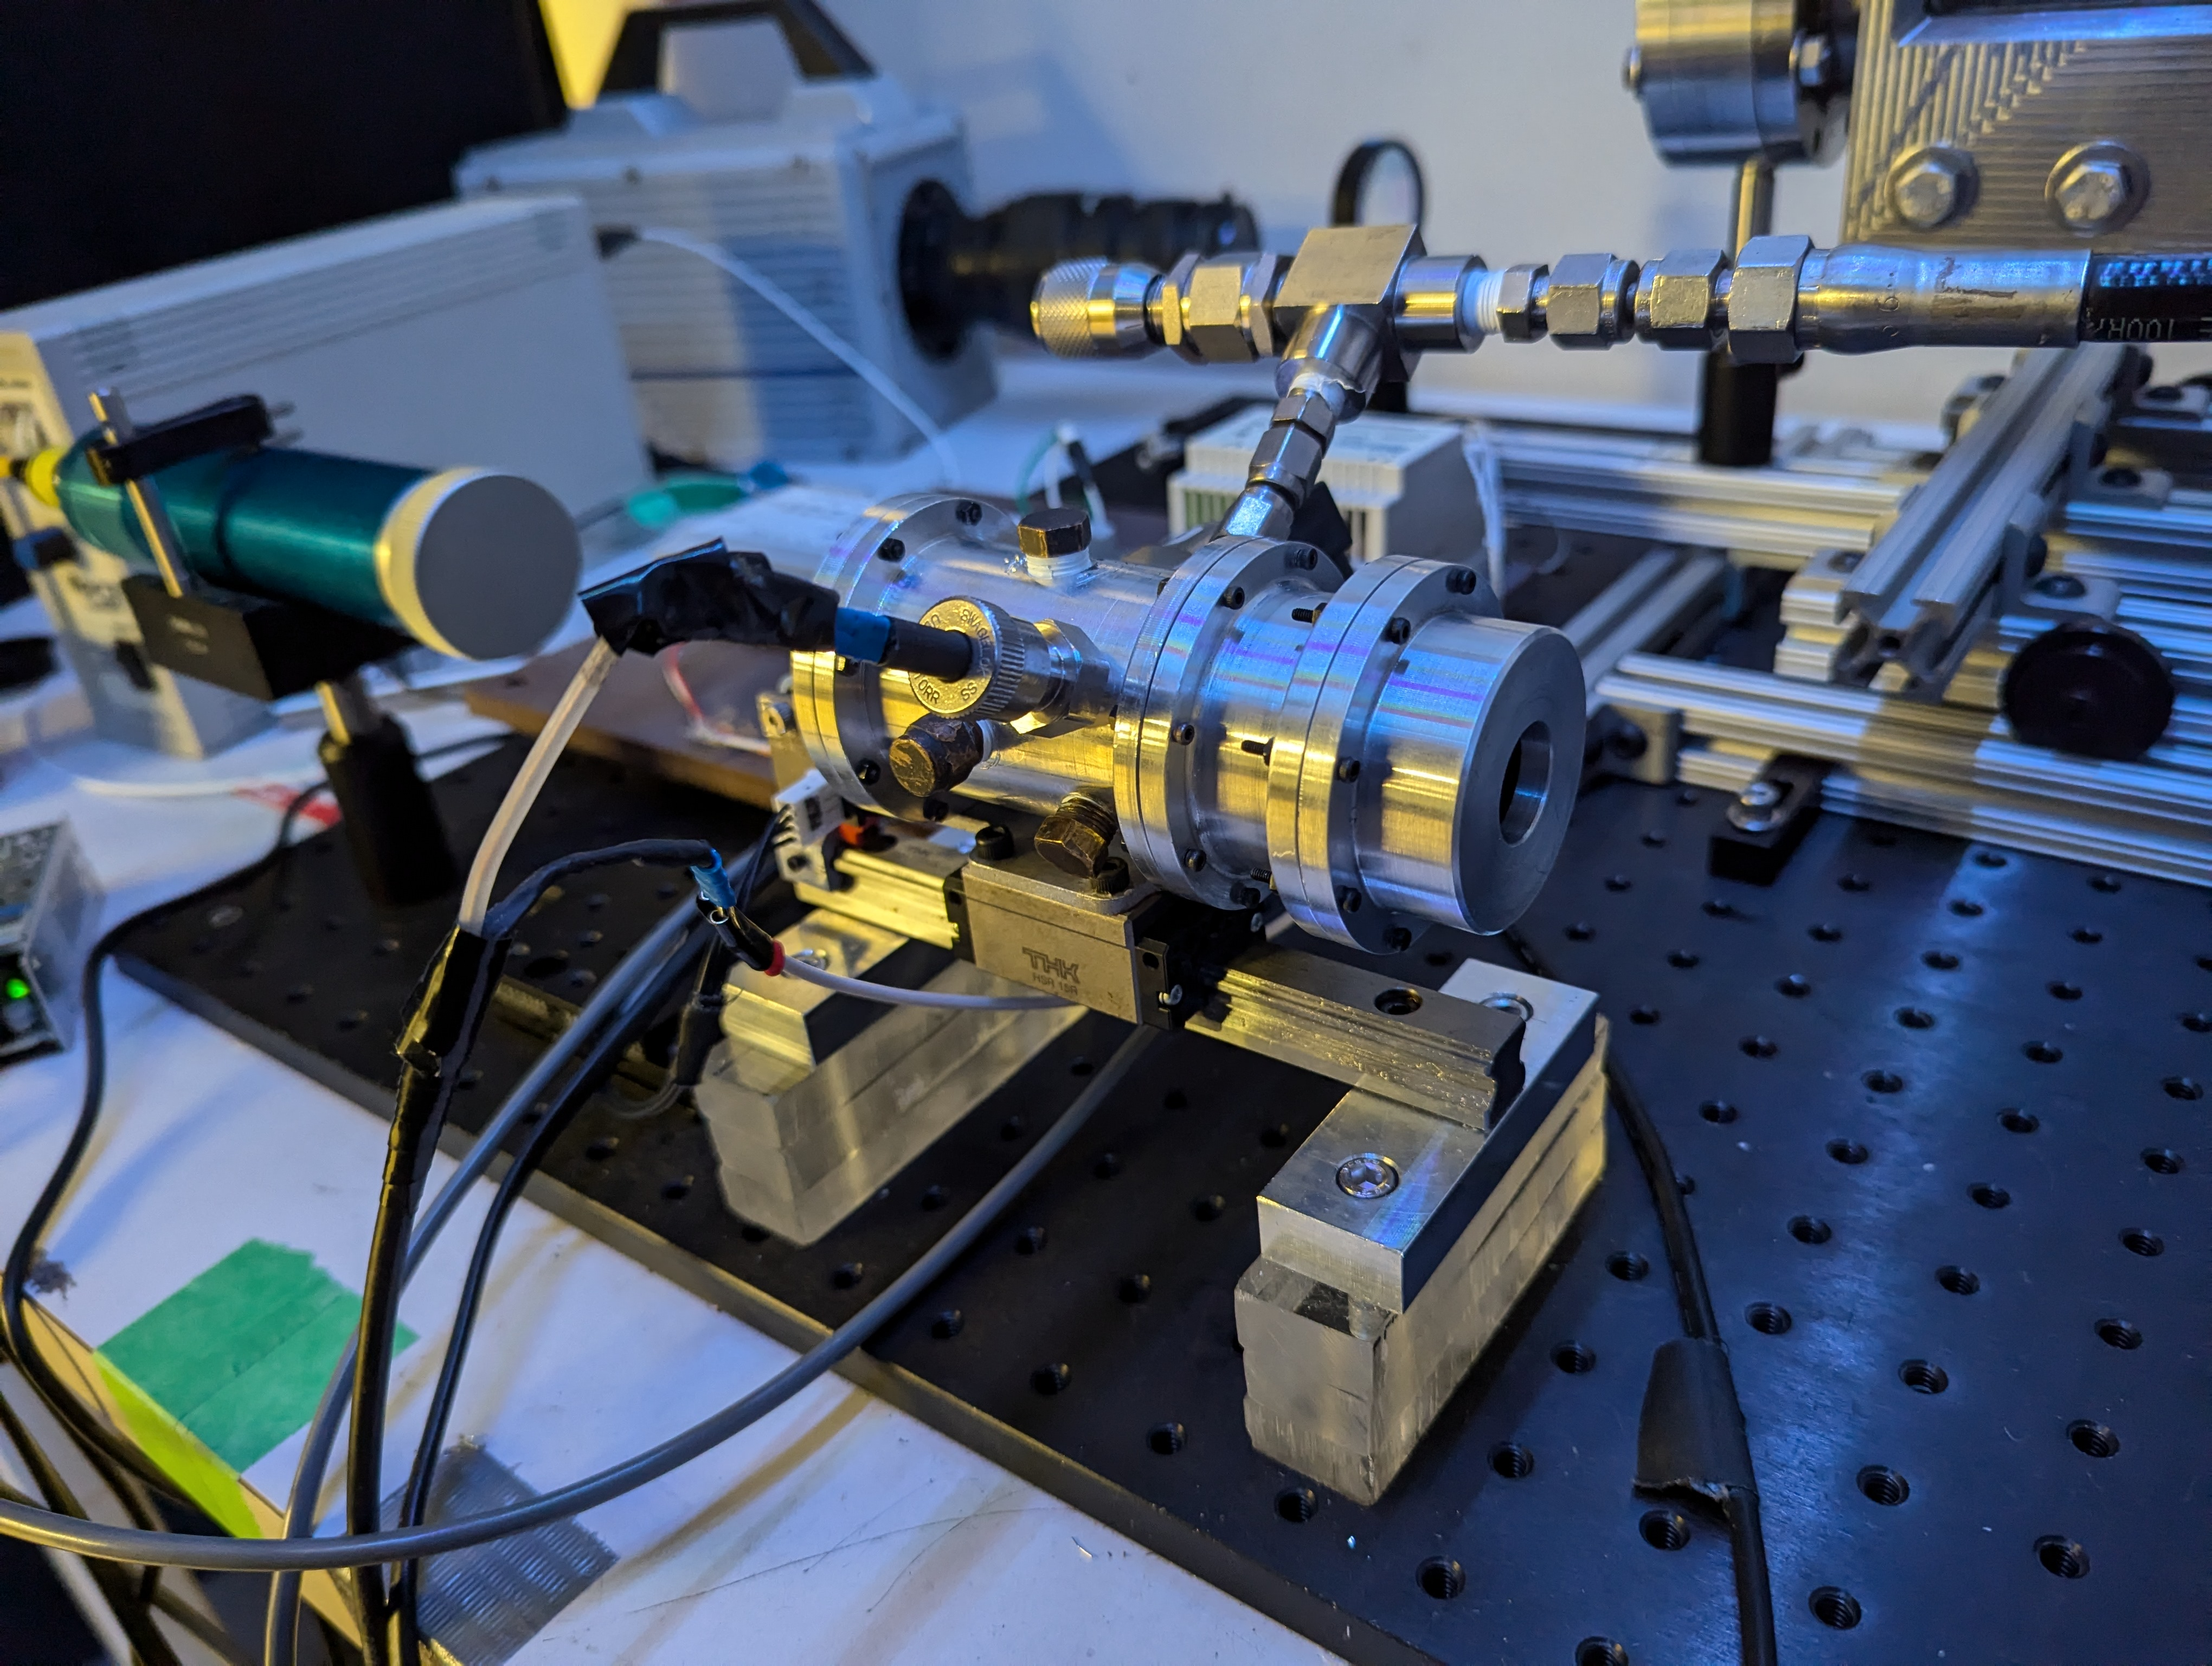
\includegraphics[width=\textwidth]{assets/3 design/V2 Static configuration.jpg}
                    \caption{Static configuration. Note the extension part and window mount.}
                \end{subfigure}
                \hfill
                \begin{subfigure}[t]{0.45\textwidth}
                    \centering
                    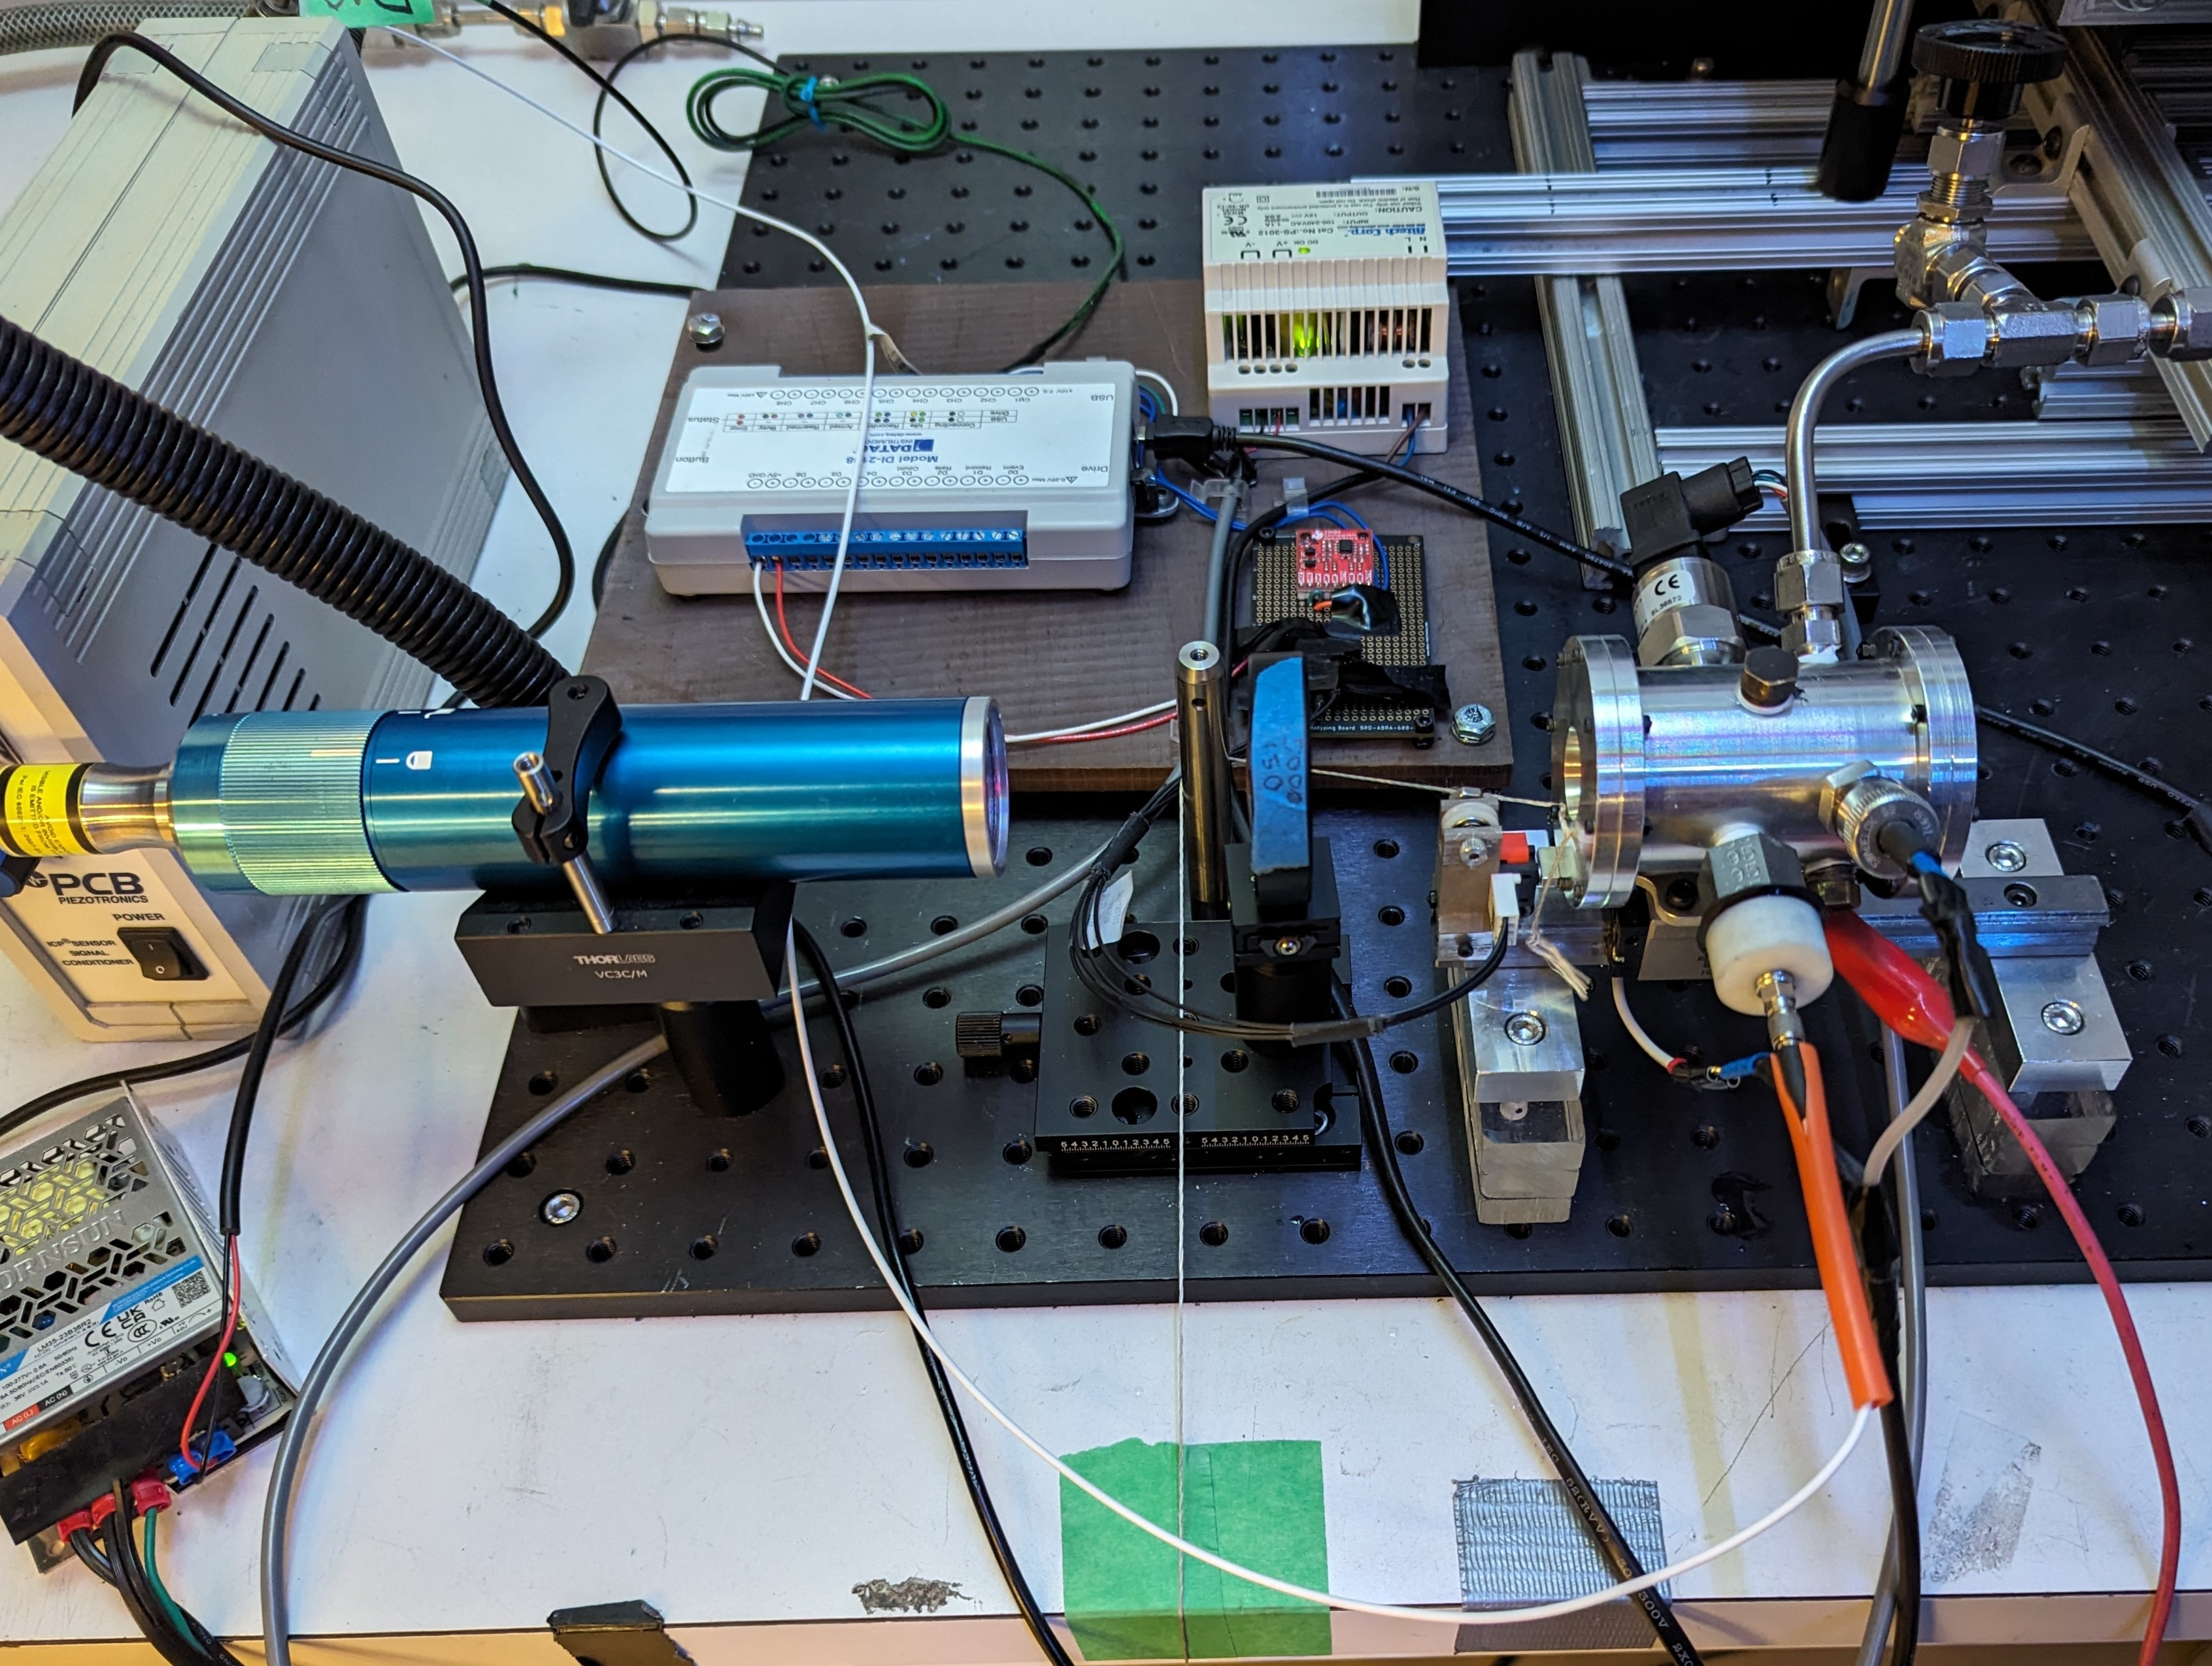
\includegraphics[width=\textwidth]{assets/3 design/V2 flowing setup.jpg}
                    \caption{Flowing configuration. The nozzle is held by the rear plate.}
                \end{subfigure}
                \caption{V2 LTP thruster}
                \label{fig:V2 setup}
            \end{figure}

            The thrust stand is a ball bearing carriage (McMaster-Carr 6709K12) mounted on a \qty{15}{mm} wide rail (McMaster-Carr 6709K33). A string through a pulley holds a variable weight, adding a preload to the test section. This ensures adequate contact between the test section and the load cell. Two load cells are used with different force sensing range: Honeywell FSG020WNPB (\qtyrange{0}{20}{N}) and Honeywell FSG005WNPB (\qtyrange{0}{5}{N}).

        \subsection{Laser}

            The laser used as the plasma's power source is an IPG Photonics YLR-300/3000-QCW-MM-AC Ytterbium fiber laser. The wavelength of the emitted light is \qty{1070}{nm}. Its nominal maximum power is \qty{3}{kW} quasi-continuous wave (QCW) or \qty{300}{W} continuous wave (CW). At \qty{3}{kW}, a QCW pulse has a maximum duration of \qty{10}{ms}. The maximum duration of a \qty{300}{W} QCW pulse is \qty{50}{ms} The laser light exits through an IPG Photonics P30-001736 collimator. The output beam is \qty{30}{mm} in diameter.

            \begin{figure}[!ht]
                \centering
                \begin{subfigure}[t]{0.45\textwidth}
                    \centering
                    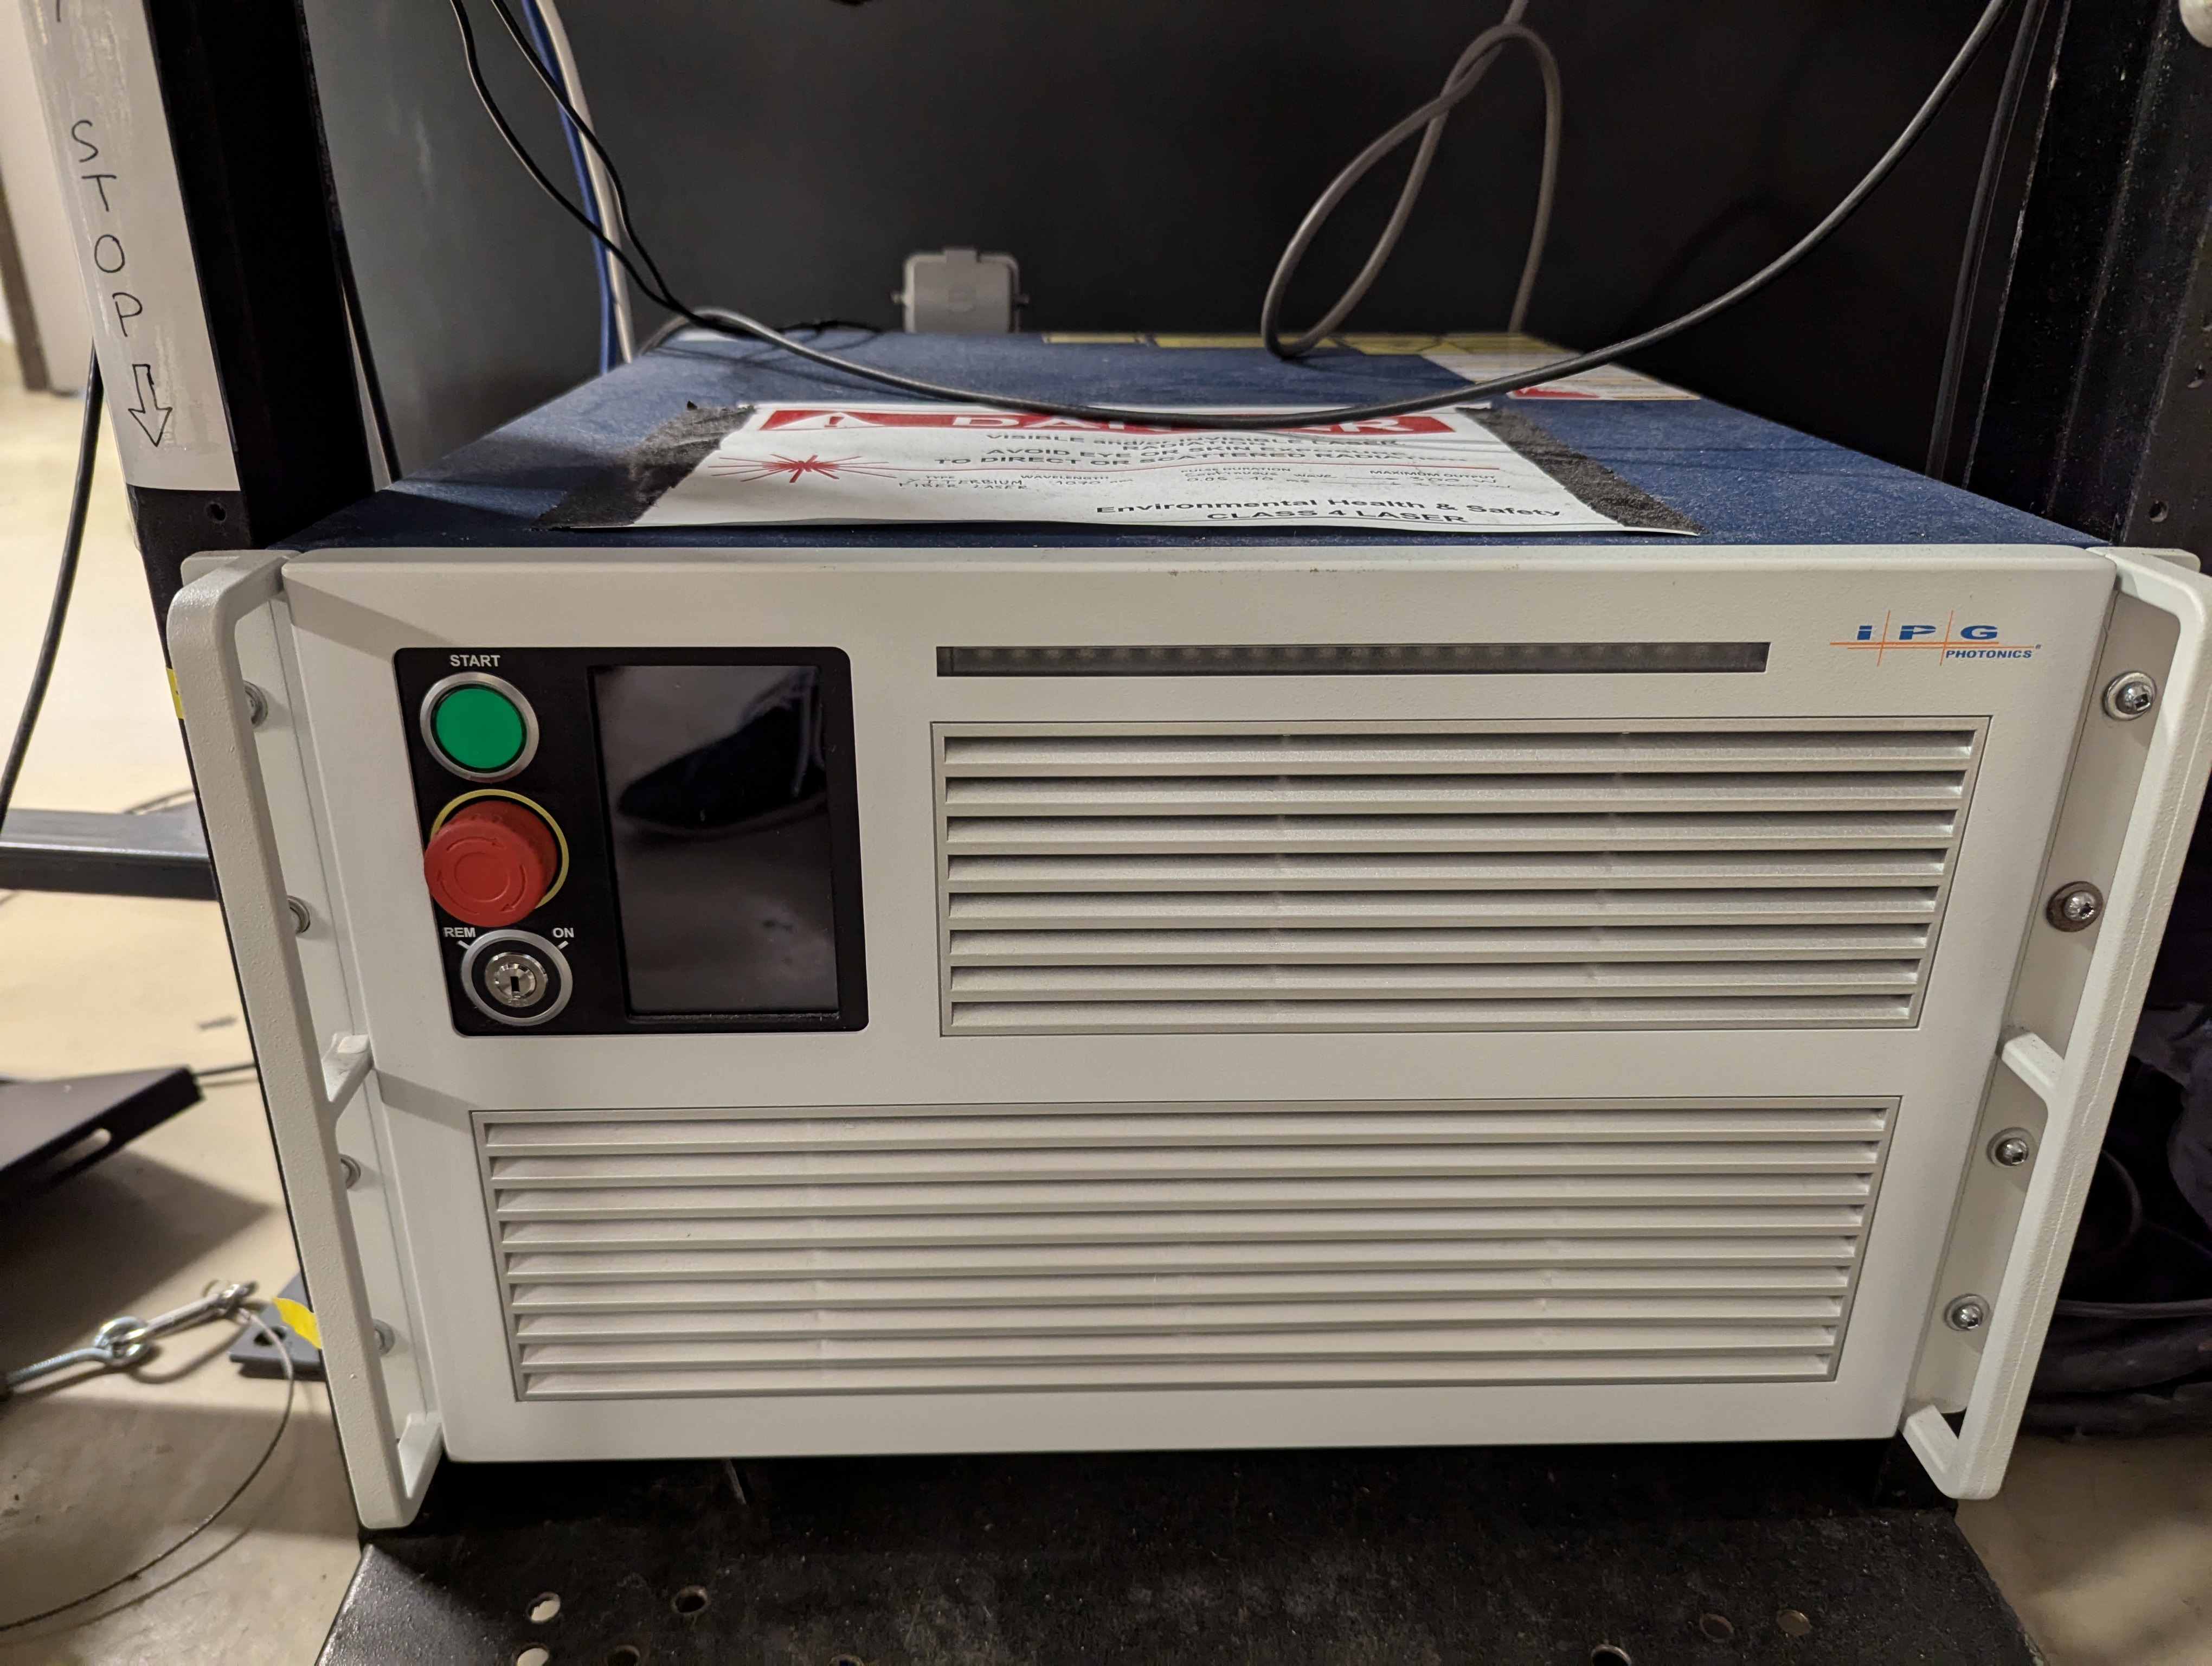
\includegraphics[width=\textwidth]{assets/3 design/Laser box.jpg}
                    \caption{IPG Photonics YLR-300/3000-QCW-MM-AC laser}
                \end{subfigure}
                \hfill
                \begin{subfigure}[t]{0.45\textwidth}
                    \centering
                    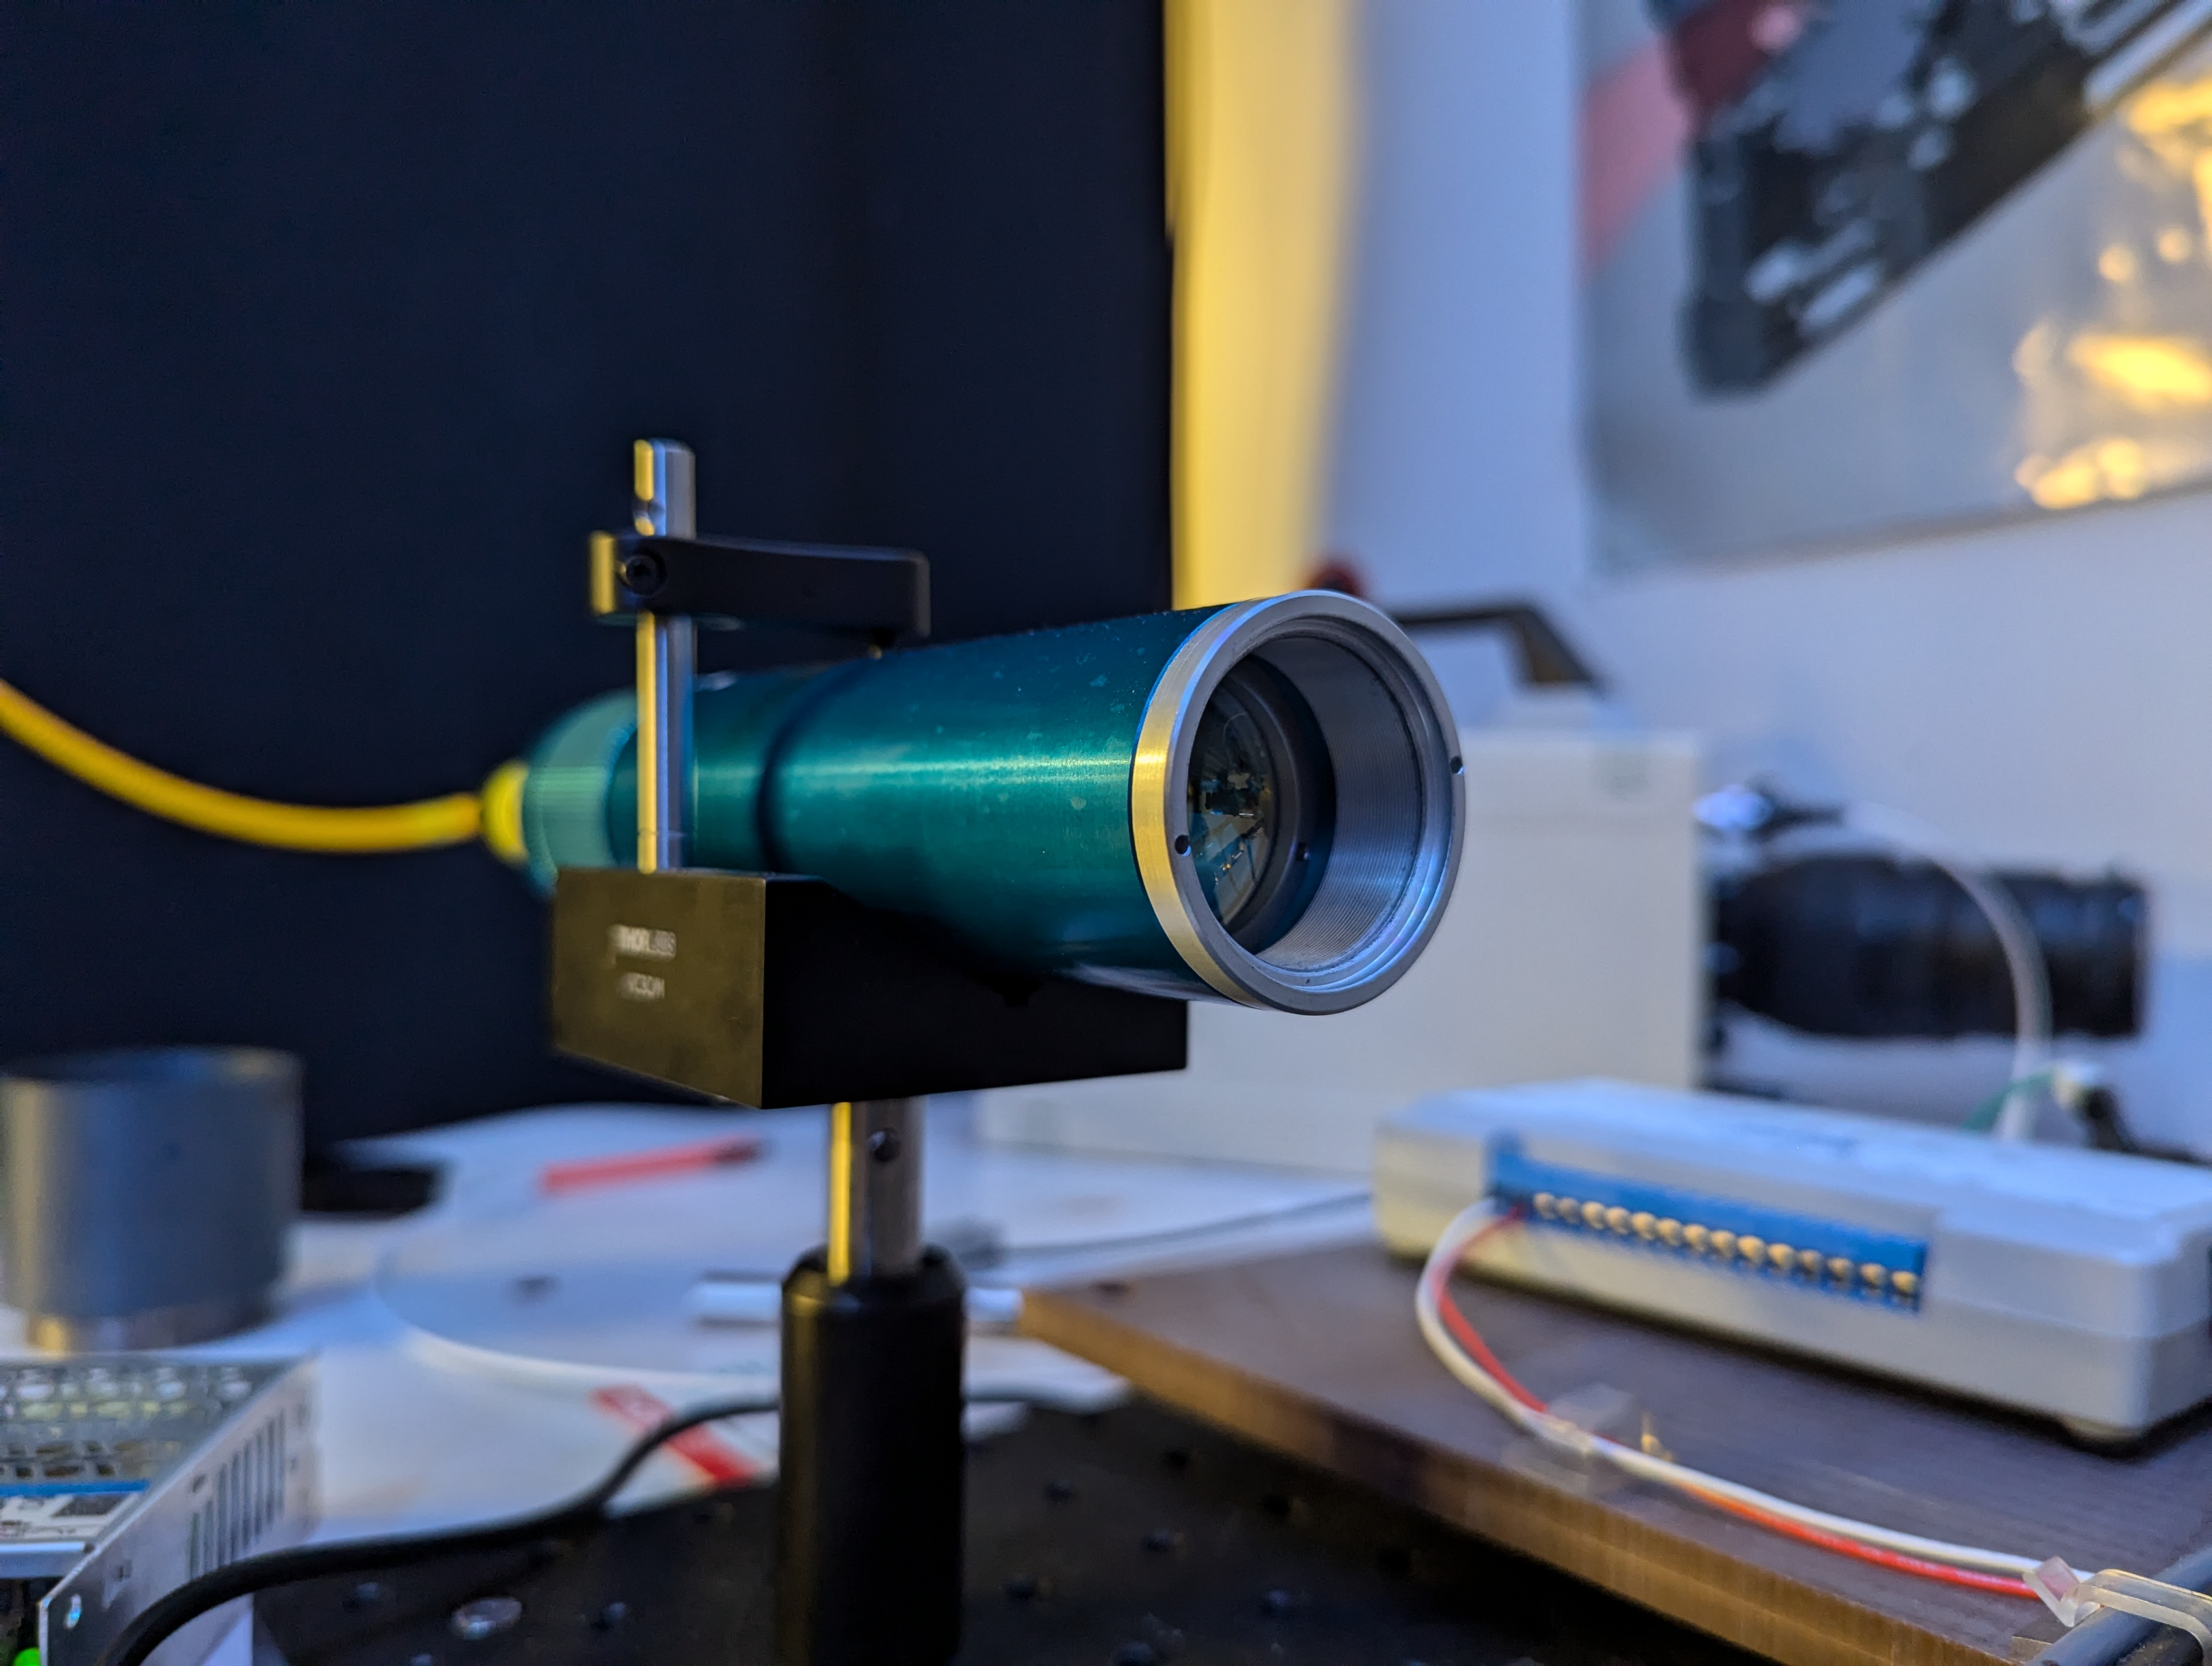
\includegraphics[width=\textwidth]{assets/3 design/Laser aperture.jpg}
                    \caption{IPG Photonics P30-001736 collimator}
                \end{subfigure}
                \caption{Laser system}
            \end{figure}

            Calibration reports for the laser and the collimator can be found in the appendix. [ADD TO APPENDIX]

        \subsection{Spark initiation system}

            AEM coil and electronics box.

        \subsection{Timing control}

            Correct timing of the laser and spark initiation is necessary to initiate LSP when the laser is in QCW mode, and to minimize damage to V2's nozzle in CW mode. To this end, delay generators are used (BNC models 7010 and 7055).

        \subsection{Data acquisition (DAQ) system and oscilloscope}

            Load cell and pressure transducer voltage is sent to a DATAQ Instruments DI-2018. This data is streamed to a personal computer by USB, where the thrust and pressure traces can be saved for analysis. Two pressure sensors were used: [PCB and OMEGA]

            \begin{figure}[!ht]
                \centering
                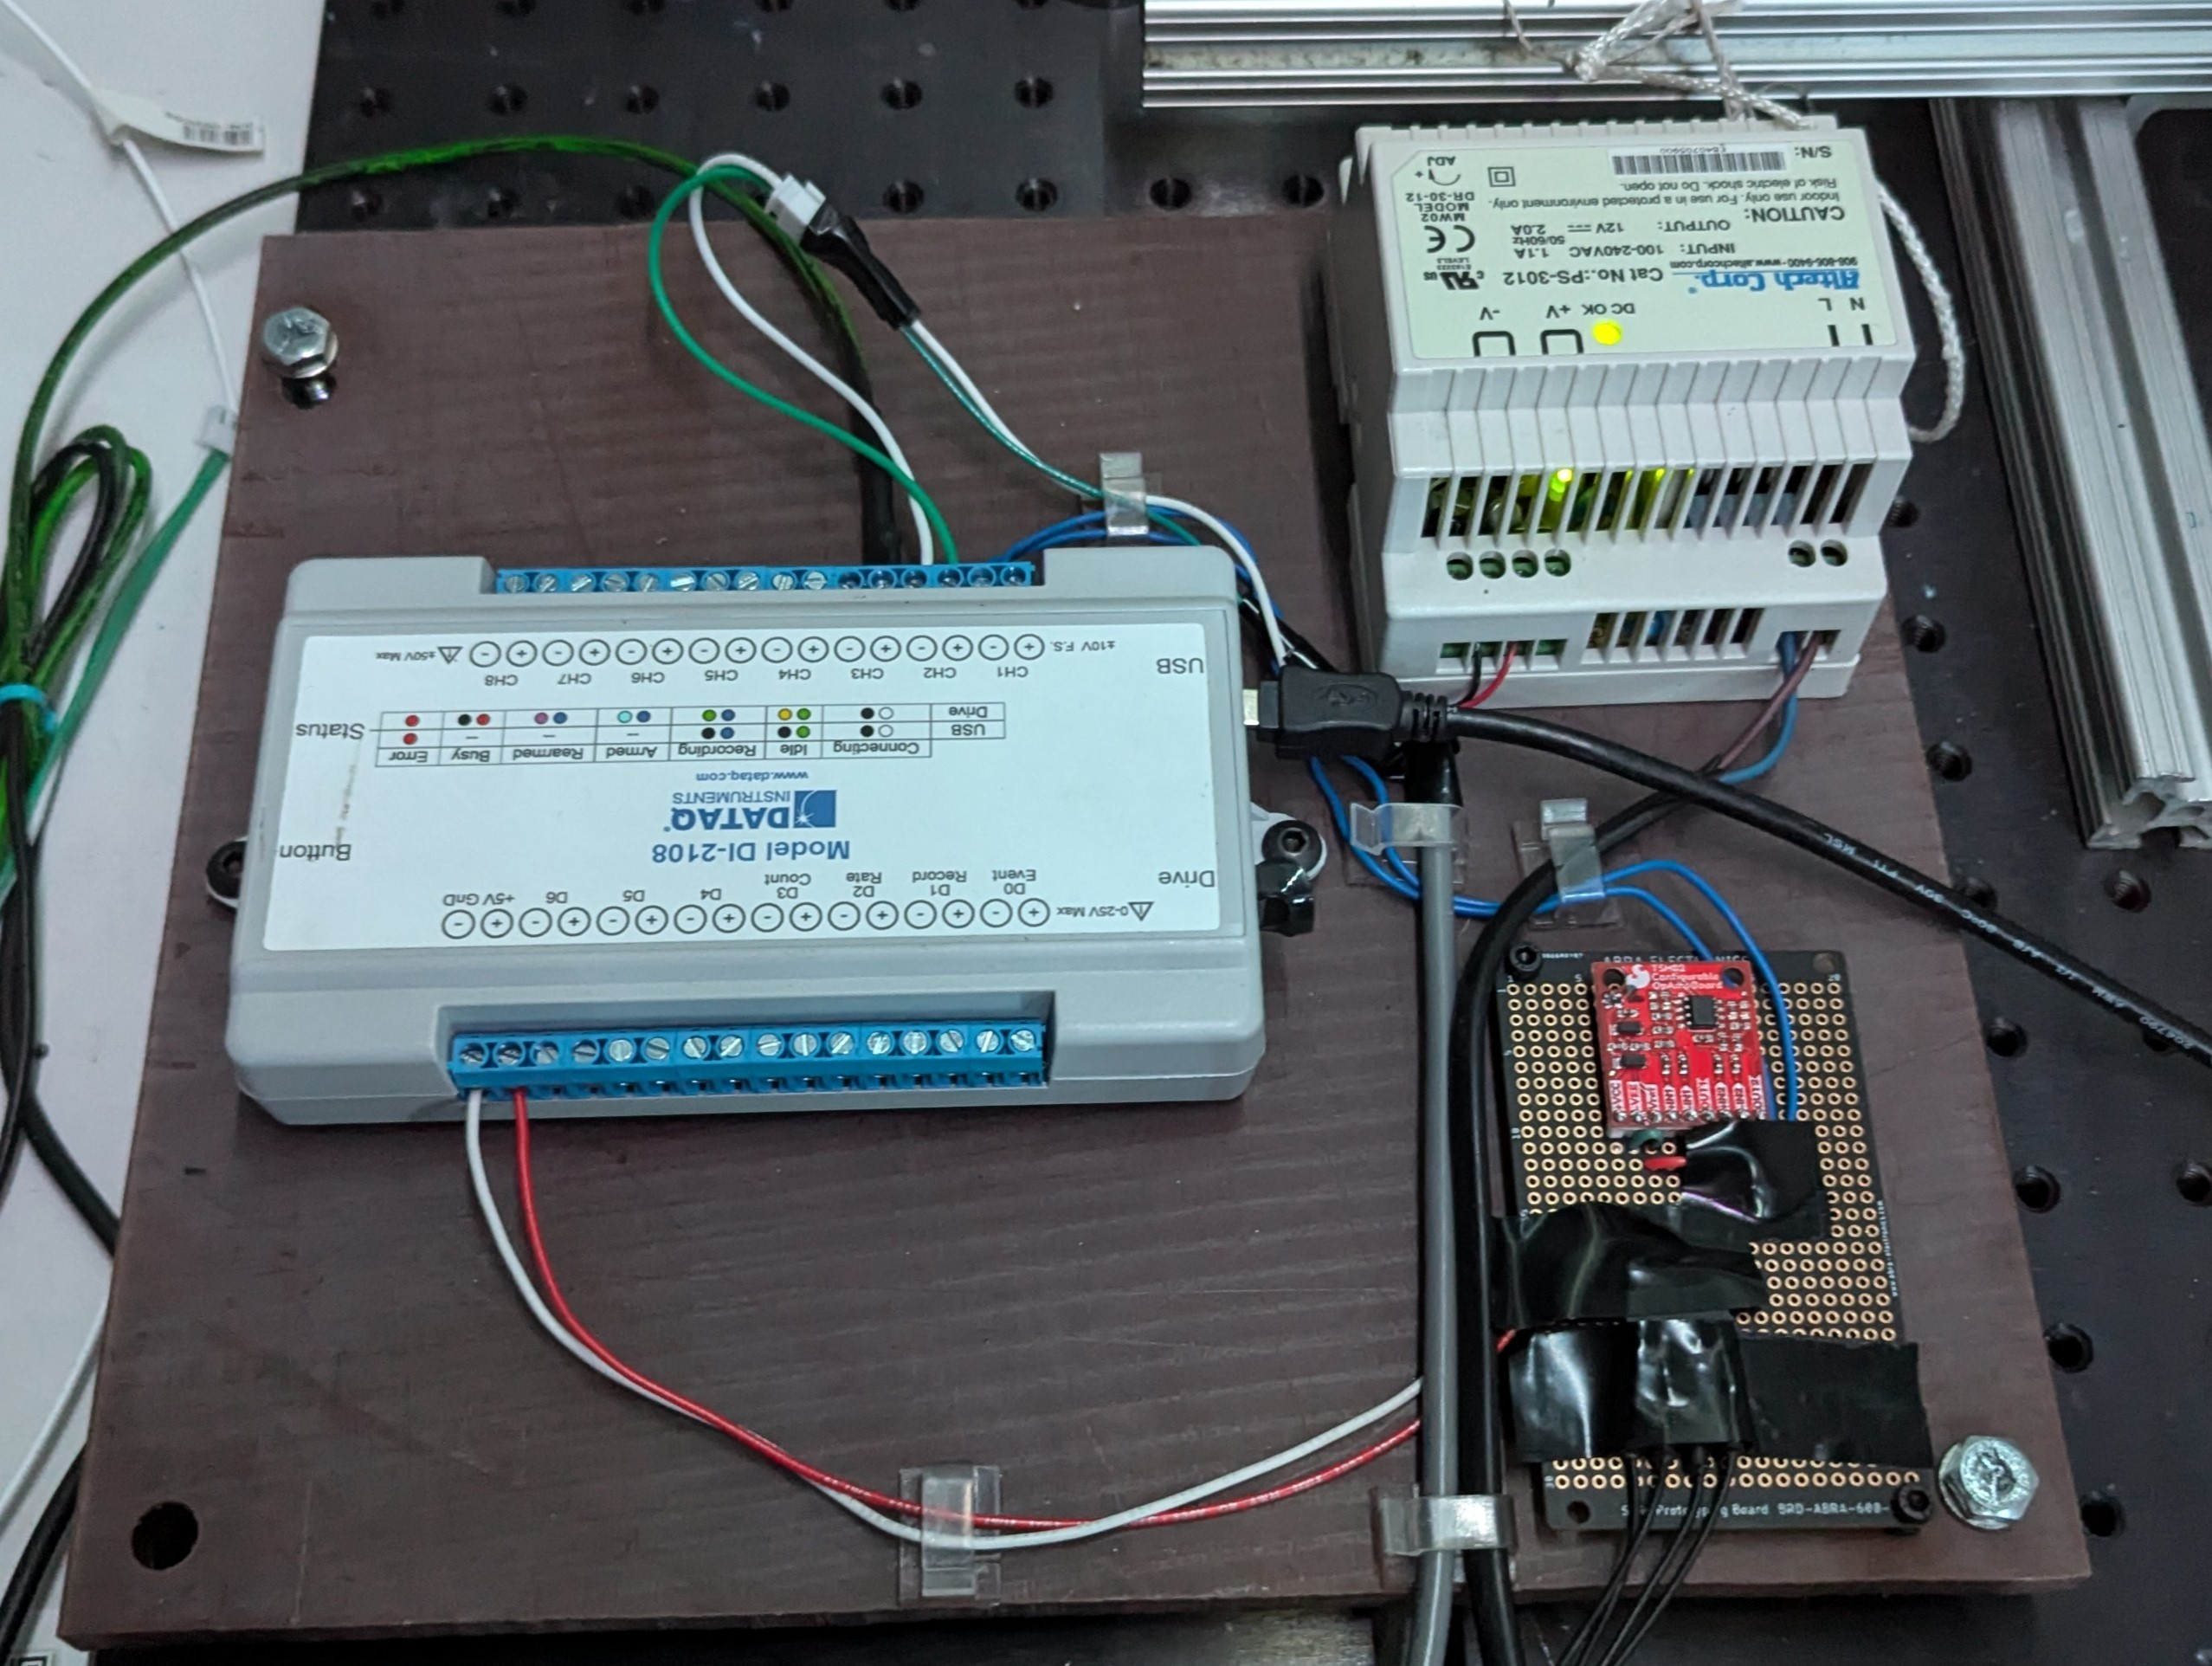
\includegraphics[width=0.50\textwidth]{assets/3 design/DAQ electronics.jpg}
                \caption{DAQ system}
                \label{fig:DAQ}
            \end{figure}

            [Photos of pressure sensor and PCB assembly]

        \subsection{High speed camera}

            A Photron SA5 high speed camera was used on certain LSP shots to validate 
            
            Due to the fact that no side window was present on V2, the Photron SA 5 high speed camera looking into the core of the thruster was used to validate.

            [Photo of Photron looking into thruster]
    \chapter{Modelling} \label{chp:models}
    Although the work of this project was primarily experimental, some modelling work was performed in order to better understand the physics of LSP and aid in the experimental design. One major area of interest is in determining the absorption properties of LSP. High laser absorption is desirable to maximize power conversion efficiency. Furthermore, the IB absorption coefficient typically reaches a maximum at a specific temperature. According to \textcite{keeferLaserSustainedPlasmas1989}, this peak absorption temperature was found to closely correlate with LSP peak temperature. The measurement of absorption coefficient can thus be used to support LSP temperature estimates.

    \section{Absorption} \label{sec:models_absorption}
        A critical property of LSP is its ability to absorb laser radiation. As stated in \autoref{sec:background_lsp}, the primary mechanism for radiation absorption in LSP is inverse bremsstrahlung. Calculation of the absorption coefficient of this process is critical for modelling LSP behavior and estimating its laser absorption efficiency. The calculation method presented here aims to adapt the work of \textcite{akarapuNumericalModelLasersustained2009,nassarInvestigationLasersustainedPlasma2012}, who have developed CFD models for the use of Argon LSP in surface-treatment applications. Although their work considered \ce{CO_2} lasers, adapting the method to the fiber laser of this study is a matter of using the appropriate laser frequency in \autoref{eq:ib_absorption}. Their work was thus used to validate each calculation step, and their results will be plotted alongside this study's computations when relevant.
        
        The absorption coefficient can be calculated using \autoref{eq:ib_absorption} and is heavily dependent on electron density $n_\mathrm{e}$ and radiation frequency $\nu$. The first step of absorption modelling is thus to determine electron density, which is variable with temperature $T$ according to the Saha ionization equation, developed by \textcite{sahaPhysicalTheoryStellar1997}. It is reproduced here for the single ionization case as \autoref{eq:saha}:
        \begin{equation}
            \frac{n_\mathrm{e}^2}{n_0-n_\mathrm{e}} = \frac{n_\mathrm{e}^2}{n_\mathrm{Ar}} = \frac{2}{\Lambda_\mathrm{th}^3}\frac{\mathcal{Z}_{\mathrm{Ar}^+}}{\mathcal{Z}_\mathrm{Ar}}\exp{\left(-\frac{E_\text{ion, Ar}}{k_\mathrm{B}T}\right)}
            \label{eq:saha}
        \end{equation}
        Where $n_0$ is the initial number density of neutral atoms, $n_\mathrm{Ar}$ is the number density of un-ionized atoms at a given temperature, $E_\text{ion, Ar}$ is Argon's first ionization energy (\qty{15.76}{eV}), and $k_\mathrm{B}$ is the Boltzmann constant. The thermal DeBroglie wavelength $\Lambda_\mathrm{th}$ is a function of temperature as follows, where $\hbar$ is the reduced Planck constant and $m_\mathrm{e}$ is the mass of an electron:
        \begin{equation*}
            \Lambda_\mathrm{th} = \sqrt{\frac{2\pi \hbar^2}{m_\mathrm{e}k_\mathrm{B}T}}
        \end{equation*}
        The ratio $\mathcal{Z}_{\mathrm{Ar}^+}/\mathcal{Z}_\mathrm{Ar}$ is the ratio of the partition function values for Ar$^+$ and Ar (also designated Ar II and Ar I, respectively). These values are also dependent on temperature and can be queried in the NIST Atomic Spectra Database (\textcite{kramidaNISTAtomicSpectra2022}) for a given spectrum (e.g., Ar I) and electron temperature $T_\mathrm{e}$. This ratio is plotted in \autoref{fig:e_density_partition}. \citeauthor{nassarInvestigationLasersustainedPlasma2012} fitted a seventh-order polynomial to approximate this ratio across temperature, which is also plotted for comparison.

        It is important to note that $n_0$ in \autoref{eq:saha} is not constant across temperatures. In the case of LSP, the ionization process occurs at constant pressure, even if the experiment occurs in a closed container, as only a small fraction of the test section volume undergoes ionization. The hotter Argon is free to expand into the cooler surroundings, locally reducing the number density and maintaining a constant pressure. Therefore, $n_0$ must be calculated based on a given pressure $p$ and the varying temperature. This can be done with the ideal gas equation, where $V$ is volume, $N$ is the number of atoms in moles, $R_\mathrm{u}$ is the universal gas constant, and $N_\mathrm{A}$ is Avogadro's number:
        \begin{align*}
            pV&= NR_\mathrm{u}T \\
            p&= \frac{N}{V}R_\mathrm{u}T \\
            \frac{N_\mathrm{A}p}{R_\mathrm{u}T}&= n_0
        \end{align*}

        The electron density $n_\mathrm{e}$ is plotted against temperature in \autoref{fig:e_density_curves}, for a pressure of \qty{1}{bar}. The calculation by \citeauthor{nassarInvestigationLasersustainedPlasma2012} is plotted alongside it, and their relative value is compared. While the electron density plots appear to agree, there remains a difference in density of a factor of two. This appears to be due to the use of lower precision physical constants in \citeauthor{akarapuNumericalModelLasersustained2009} and \citeauthor{nassarInvestigationLasersustainedPlasma2012}'s work.

        \begin{figure}[h]
            \centering
            \begin{subfigure}[t]{2.6in}
                \centering
                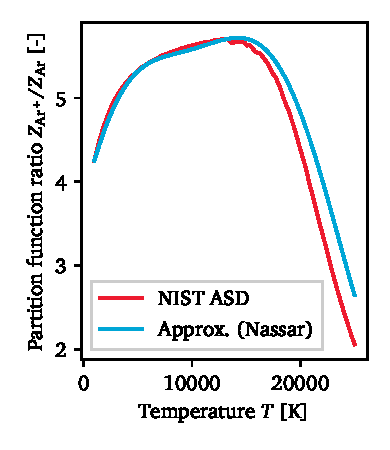
\includegraphics[]{assets/4 models/partition}
                \caption{Ratio of Ar II to Ar I partition function values}
                \label{fig:e_density_partition}
            \end{subfigure}
            \hfill
            \begin{subfigure}[t]{3.2in}
                \centering
                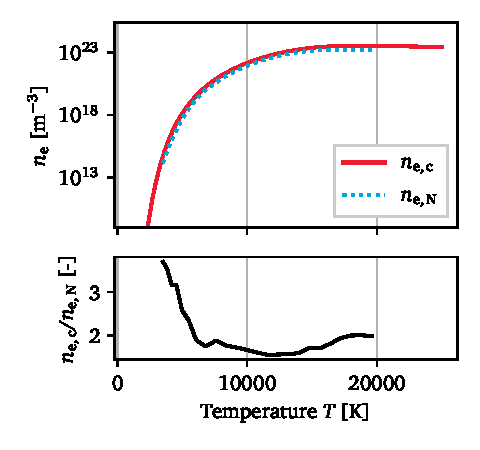
\includegraphics[]{assets/4 models/n_e}
                \caption{$n_e$ at \qty{1}{bar}, and comparison between computed density $n_\mathrm{e, c}$ and density $n_\mathrm{e, N}$ reported by \textcite{nassarInvestigationLasersustainedPlasma2012}}
                \label{fig:e_density_curves}
            \end{subfigure}
            \caption{Computation of electron density $n_\mathrm{e}$ of Argon}
            \label{fig:e_density}
        \end{figure}

        Although electron density appears to plateau past \qty{20000}{K}, the caveat of this calculation is that it only considers single-ionization. While this is valid below \qty{20000}{K}, second-degree ionization begins past this temperature. The plot is extended up to \qty{25000}{K} to provide some estimate of plasma properties, although they will not be as accurate as below \qty{20000}{K}.

        The absorption coefficient $\alpha$ can now be calculated with the known electron density. For convenience, the equation for $\alpha$, \autoref{eq:ib_absorption}, is reproduced here:
        \begin{equation*}
            \ibalphaeq \tag{\ref{eq:ib_absorption} revisited}
        \end{equation*}
        Most parameters have been defined in \autoref{sec:background_lsp}, so the Coulomb logarithm $\ln{\Lambda}$ and the plasma frequency $\nu_\mathrm{p}$ will be of interest here. The Coulomb logarithm is evaluated by \textcite{nassarInvestigationLasersustainedPlasma2012} using a common approximation seen in plasma physics (\textcite{richardson2019NRLPlasma2019}):
        \begin{equation}\label{eq:coulombLog_NRL}
            \ln{\Lambda} \approx 23-\ln{(n_\mathrm{e}^{1/2}ZT_\mathrm{e}^{-3/2})}
        \end{equation}
        However, alternate evaluations of the logarithm exist, such as the one given by \textcite{johnstonCorrectValuesHighfrequency1973} in the specific context of IB absorption coefficient calculation (\autoref{eq:coulombLog_johnston}). 
        \begin{equation} \label{eq:coulombLog_johnston}
            \Lambda(\nu) = \begin{cases}
                \frac{v_T}{\nu\rho_\mathrm{min}} & \nu \gg \nu_\mathrm{p}\\
                \frac{v_T}{\nu_\mathrm{p}\rho_\mathrm{min}} & \text{otherwise}
            \end{cases}
        \end{equation}
        Where $v_T$ is the electron thermal velocity, $\nu$ is the laser frequency, $\nu_\mathrm{p}$ is the plasma frequency, and $\rho_\mathrm{min}$ is the impact parameter. These can be evaluated with the following equations:
        \begin{gather}
            v_T = \sqrt{\frac{k_\mathrm{B}T}{m_\mathrm{e}}} \\
            \nu_\mathrm{p} = \frac{1}{2\pi}\sqrt{\frac{e^2n_\mathrm{e}}{\epsilon_0 m_\mathrm{e}}} \approx (\qty{8.97885}{m^{3/2}s^{-1}})\sqrt{n_\mathrm{e}}\\
            \rho_\mathrm{min} \approx \max{\left(\frac{Ze^2}{k_\mathrm{B}T}, \frac{\hbar}{(m_\mathrm{e}k_\mathrm{B}T)^{1/2}}\right)}
        \end{gather}
        \textcite{johnstonCorrectValuesHighfrequency1973} state:
        \begin{quote}
            ...at frequencies well above the plasma frequency $\nu_\mathrm{p}$, $\ln{\Lambda}(\nu)$ should contain the wave frequency $\nu$ rather than the plasma frequency $\nu_\mathrm{p}$.
        \end{quote}
        The respective frequencies of the plasma, \ce{CO_2} laser, and fiber laser are plotted in \autoref{fig:coulomb_freq} for comparison. It can be seen that for a fiber-laser-powered LSP, the $\nu \gg \nu_\mathrm{p}$ case of \autoref{eq:coulombLog_johnston} is valid across the range of temperatures of interest, so \citeauthor{johnstonCorrectValuesHighfrequency1973}'s statement is highly relevant in this case, and perhaps of lesser importance in \citeauthor{nassarInvestigationLasersustainedPlasma2012}'s study. As it was not clear whether the approximation of $\ln{\Lambda}$ in \autoref{eq:coulombLog_NRL} was applicable in this case, both evaluations of the Coulomb logarithm were compared in \autoref{fig:coulomb_coulomb}, showing that while there is a large divergence at lower temperatures, this is negligible as the Argon is not in a plasma state. For temperatures of interest, namely above \qty{10000}{K}, both evaluations of the Coulomb logarithm appear to converge. \citeauthor{johnstonCorrectValuesHighfrequency1973}'s form of the logarithm was retained for further calculations as it considers the relative values of the plasma and laser frequencies.

        \begin{figure}[h]
            \centering
            \begin{subfigure}[t]{2.9in}
                \centering
                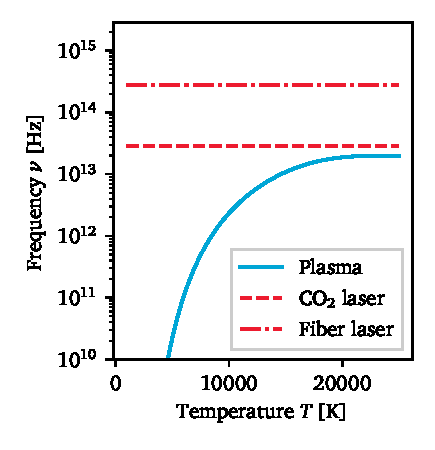
\includegraphics[]{assets/4 models/frequency_comparison}
                \caption{Comparison of plasma and laser frequencies}
                \label{fig:coulomb_freq}
            \end{subfigure}
            \hfill
            \begin{subfigure}[t]{2.9in}
                \centering
                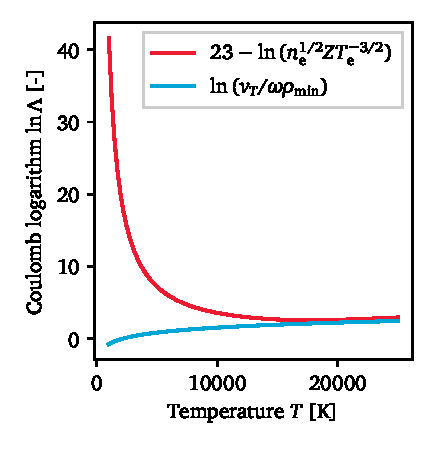
\includegraphics[]{assets/4 models/coulombLog}
                \caption{Comparison of computation methods}
                \label{fig:coulomb_coulomb}
            \end{subfigure}
            \caption{Calculation of the Coulomb logarithm, \qty{10}{bar}}
            \label{fig:coulomb}
        \end{figure}

        With values for the Coulomb logarithm and the plasma frequency, \autoref{eq:ib_absorption} can be evaluated. \autoref{fig:ib_coeff} plots the IB absorption coefficient for a range of temperatures and pressures. The point of peak absorption appears around the \qty{20000}{K} mark, with a sharp rise in peak absorption coefficient with increasing pressure. This is expected as $\alpha$ is proportional to $n_\mathrm{e}^2$ on the first order, which increases with pressure. The occurrence of peak absorption appears to shift to greater temperatures as pressure increases.

        \begin{figure}[h]
            \centering
            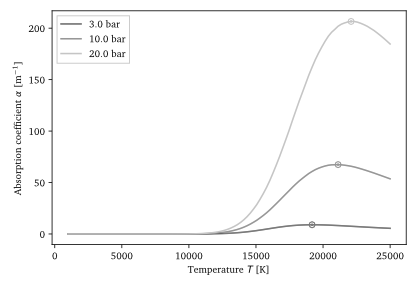
\includegraphics[]{assets/4 models/absorption}
            \caption{Inverse bremsstrahlung absorption coefficient of Argon at various pressures, \qty{1070}{nm} radiation}
            \label{fig:ib_coeff}
        \end{figure}

        The temperature of peak absorption is of interest, as it correlates to the peak temperature of the LSP (\textcite{keeferLaserSustainedPlasmas1989}). This absorption model thus suggests that a peak temperature of around \qty{20000}{K} should be expected.
    \chapter{Experiments}
    The results of the first experiments performed on the LSP facility are presented here. These include an exploration of ignition methods and their reliability, the attempted replication of power-threshold experiments seen in LSP literature, and the analysis of LSP's absorption, heat deposition, and spectral characteristics. Preliminary flowing data is also presented and contrasted with the static case.

    \autoref{fig:finalsetup_static} provides an overview of the instrumentation used in static experiments and their relative positions.

    \begin{figure}[h]
        \centering
        \includegraphics[width=0.85\textwidth]{assets/5 results/finalsetup_static}
        \caption{Static configuration of the test section}
        \label{fig:finalsetup_static}
    \end{figure}

    \section{Preliminary ignition experiments} \label{sec:ignitiontest}
        Once the necessary components of the experiment were integrated, a preliminary testing campaign began to attempt to ignite LSP. The hope was to resolve any unforeseen practical issues, then quickly move on to replicating the power threshold experiments of past LSP literature~\cite{zimakovInteractionNearIRLaser2016,matsuiGeneratingConditionsArgon2019,luCharacteristicDiagnosticsLaserStabilized2022}. The test campaign aimed to answer two questions:
        \begin{itemize}
            \item Can LSP be achieved with this experimental setup at all?
            \item How reliable is LSP ignition with this system?
        \end{itemize}
        To answer this, experimental trials would be run in conditions most favorable to steady LSP formation, i.e. at maximum laser power and maximum test section pressure: \qty{3}{kW} and \qty{20}{bar}. Successful ignition would be determined based on two independent measures:
        \begin{enumerate}
            \item The high-speed camera should be able to image the LSP growing and propagating towards the laser source over the course of the laser pulse, as consistently documented in LSP literature.
            \item A measurable drop in laser energy reaching the Gentec power meter should be observed.
        \end{enumerate}
        LSP would only be deemed to have successfully ignited if the expected behavior was observed with both instruments.

        \subsection{Spark-ignition}
            Laser alignment was immediately found to be a non-trivial problem. In order to successfully ignite the LSP, the laser must be focused onto the arc generated by the spark igniter. To maximize the chance of ignition, the laser flux at the arc must be as high as possible, so the focused laser dot must be as small as possible. This makes alignment tolerances much stricter, as the laser is less likely to be incident on the thin arc at all.

            Compounding this issue was the fact that the path taken by the arc between both electrode tips was not consistent. As seen in \autoref{fig:sparkAlignment}, the location of the arc was highly variable: though an average arc path could be determined, the arc could form up to \qty{1}{mm} away. This made it impossible to ensure consistent alignment between the arc and the laser focus. This issue could be alleviated by repeatedly triggering the spark, but the smart coil had a nominal delay of \qty{3}{ms} between sparks, only allowing up to three ignition attempts within a single laser pulses, making this approach of little viability for high-power pulse laser tests. Repeated sparks could be used with CW laser operation at \qty{300}{W}, but the lower laser power also reduces the likelihood of successful LSP ignition.

            \begin{figure}[h]
                \centering
                \begin{subfigure}[t]{0.47\textwidth}
                    \centering
                    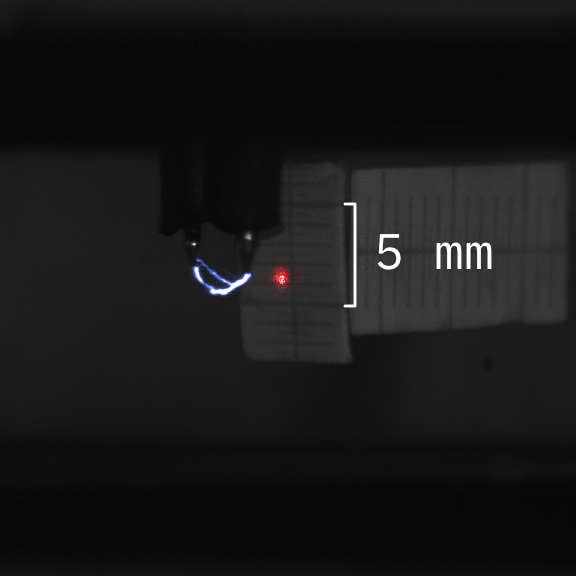
\includegraphics[]{assets/3 design/sparkAlignment_one.jpg}
                    \caption{Single arc generated by the spark igniter}
                    \label{fig:sparkAlignment_one}
                \end{subfigure}
                \hfill
                \begin{subfigure}[t]{0.47\textwidth}
                    \centering
                    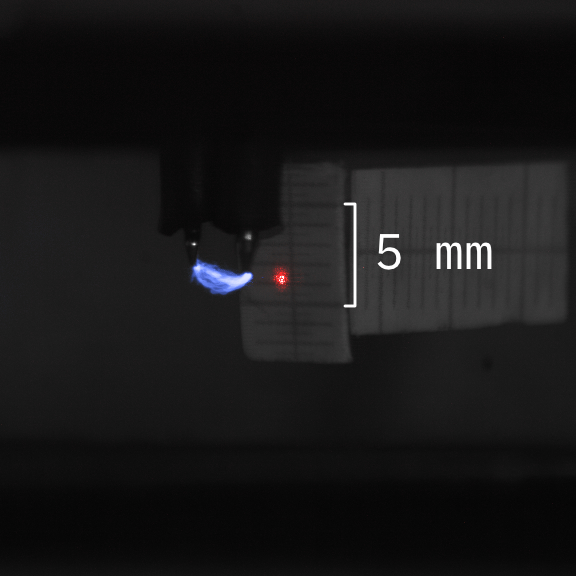
\includegraphics[]{assets/3 design/sparkAlignment.jpg}
                    \caption{Several arcs stacked together to create a ``heatmap'' of arc formation. Note the large variance in the path taken by the arc.}
                    \label{fig:sparkAlignment_heatmap}
                \end{subfigure}
                \caption[Composite photos made during a typical spark-laser alignment procedure]{Composite photos made during a typical spark-laser alignment procedure. The gray-scale background, blue arcs, and red guide laser photos were taken separately then stacked together to be able to compare the relative position of the arcs and laser.}
                \label{fig:sparkAlignment}
            \end{figure}

            In addition, the laser could not be aligned without placing reflecting or scattering material in the beam path. As seen in \autoref{fig:sparkAlignment}, a target must be placed near the ignition point to perform the alignment (and also serves as a scale indicator). However, this alignment target had to be removed to pressurize the test section, which was required both to determine the spark location, and to perform the LSP ignition test. Pressurization cycles and the placing/removal of this target made the alignment process slow and cumbersome. Alignment with the arcs could not be confirmed visually since the target could not be present when pressurizing the test section.

            Despite these difficulties, several attempts were made to ignite LSP with this method, and a few were successful. The first successful test was performed at \qty{10.02}{bar} with a full power pulse (\qty{30.8}{J}). A paper target had been placed next to the electrodes to facilitate alignment, so no measurements were made of the pulse energy transmitted through the plasma for the first few successful tests. However, high-speed footage showed strong evidence of plasma formation: a bright flash saturating the camera sensor, igniting at the time of spark formation, as seen in \autoref{fig:lsp1}. Such a flash had never been observed in past (failed) ignition tests. Though this suggested that some plasma had been formed, there was a possibility that the alignment target was affecting the experiment and may even have contributed to the ignition. The footage showed evidence of particles being ejected from the area around the ignition point, possibly due to the interaction between the laser, plasma, and the paper target.

            \begin{figure}[h]
                \centering
                \begin{subfigure}[t]{0.32\textwidth}
                    \centering
                    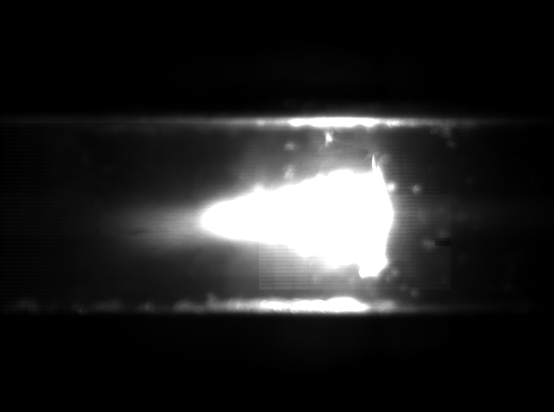
\includegraphics[width=\textwidth]{assets/3 design/LSP1_frames/20.jpg}
                    \caption{2.0~ms}
                    \label{fig:lsp1_20}
                \end{subfigure}
                \hfill
                \begin{subfigure}[t]{0.32\textwidth}
                    \centering
                    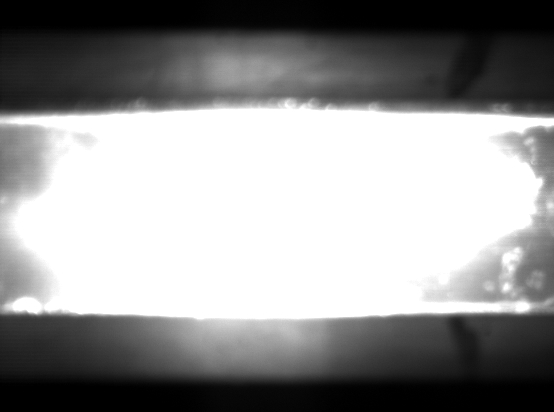
\includegraphics[width=\textwidth]{assets/3 design/LSP1_frames/30.jpg}
                    \caption{3.0~ms}
                    \label{fig:lsp1_30}
                \end{subfigure}
                \hfill
                \begin{subfigure}[t]{0.32\textwidth}
                    \centering
                    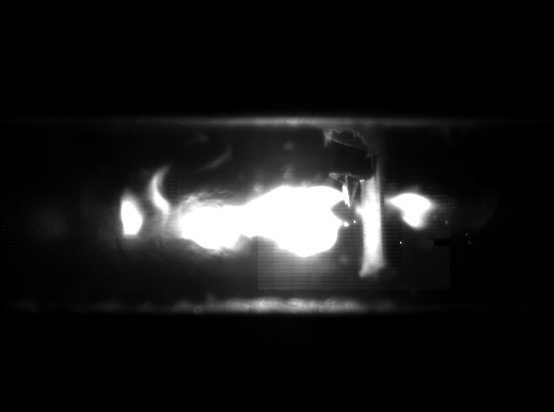
\includegraphics[width=\textwidth]{assets/3 design/LSP1_frames/75.jpg}
                    \caption{7.5~ms}
                    \label{fig:lsp1_75}
                \end{subfigure}
                \caption{High-speed footage frames of first successful LSP ignition}
                \label{fig:lsp1}
            \end{figure}

            The experiment was repeated with the target several times, ensuring that the flash was not the result of merely burning a hole through the paper target. In addition, the exposure settings were adjusted (increasing the ND filter to ND2048 and setting the aperture to \textit{f}/22) to provide a clearer view of the brightest part of the frame, the LSP core. A snapshot of the resulting footage is shown in \autoref{fig:lsp3}, revealing a slender plasma core, approximately contained within the focused laser beam (note the thinner right tip of the LSP compared to the left tip). The plasma was observed to grow towards the source of the laser, as reported in experimental LSP literature. This appearance and growth behavior provided additional evidence that these tests were truly achieving laser-sustained plasma, as opposed to some other phenomenon.

            \begin{figure}[h]
                \centering
                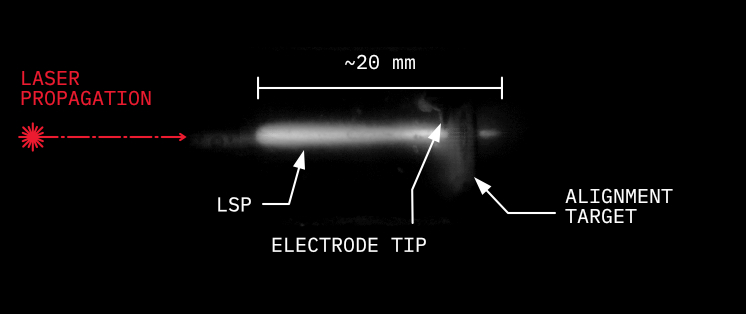
\includegraphics[]{assets/3 design/LSP3_annotated.jpg}
                \caption[Third successful LSP test ignited by arc discharge]{Third successful LSP test ignited by arc discharge. Snapshot from just before the end of the laser pulse. Dimension is approximate.}
                \label{fig:lsp3}
            \end{figure}

            To provide complete confidence that this indeed was LSP, more experiments were performed without the paper target. This allowed the measurement of the laser energy not absorbed by the plasma, and would confirm that the LSP is ignited purely by the spark, as opposed to ablated material from the paper target. With a fully uninterrupted beam path, the power meter reported a 70 to 80~\% drop in laser pulse energy during a test, suggesting that significant laser absorption was occuring in the plasma. This thus satisfied the second criterion for determining successful LSP ignition.

        \subsection{Wire-ignition}
            As power-threshold experiments were underway, as discussed in \autoref{sec:results_powerthreshold}, it became apparent that the reliability of spark-ignition was unsatisfactory. The inability to consistently arc through the laser beam meant that most ignition attempts would fail, especially below full laser power. Reliability of the spark ignition system was estimated between 10~\% and 50~\% depending on conditions.

            Private communications with Prof. Todd and Dr. Nassar (involved in \cite{akarapuNumericalModelLasersustained2009,nassarInvestigationLasersustainedPlasma2012}) highlighted the difficulty of spark ignition, and motivated the change to a solid-target system, with the use of thin metallic wire as an ignition target. Tungsten had been used successfully in past LSP experiments, such as those of \textcite{toyodaThrustPerformanceCW2002}, so \qty{0.254}{mm} (0.01") Tungsten wire was acquired and placed in the beam path as a target.

            Wire-ignition proved to be easier to work with, as laser alignment was simpler. However, it did not guarantee ignition either---wire ignition's greater reliability revealed other important factors in consistently achieving LSP:
            \begin{itemize}
                \item Axial positioning of the laser focus such that it coincides with the target is crucial to generate the ``seed'' cloud of electrons necessary for LSP ignition.
                \item Ensuring high Argon purity in the chamber was also found to be important. Venting of residual air in the system done by performing several pressurization-vent cycles with Argon---at least 3 cycles up to \qty{5}{bar}---before final pressurization to the test pressure. While this was sufficient for tests at \qty{10}{bar} and above, additional cycles were found to improve ignition reliability at low pressures (\qtyrange{3}{10}{bar}).
            \end{itemize}
            Factors that were hypothesized to impact reliability but ultimately were found to have little to no impact include:
            \begin{itemize}
                \item Focusing the laser on the same spot on a wire across several tests
                \item Touching/dirtying the wire before installing it in the test section
                \item Sanding/cleaning the wire before installing it in the test section
            \end{itemize}
            Once these reliability factors were identified and controlled, wire ignition proved to be highly reliable, attaining practically 100~\% reliability.

        \subsection{Early LSP observations}
            These early ignition tests already allowed the observation of LSP. \autoref{fig:ignition_frames} depicts the initial growth of LSP ignited off a Tungsten wire, showing rapid growth over a fraction of a millisecond. Under the right ignition conditions, plasma would form practically as soon as the laser was turned on, before the Tungsten wire had time to heat up and melt off. This quick ignition would prove to be a useful property when combined with stepped-pulse profiles in later power threshold experiments.

            \begin{figure}[h]
    \centering
    \begin{subfigure}[t]{0.3\textwidth}
        \centering
        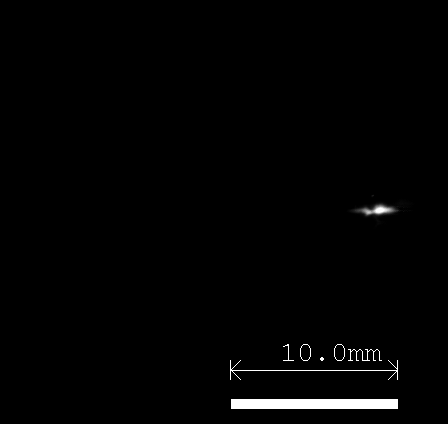
\includegraphics[width=\textwidth]{assets/4 experiments/V1 Spark Ignition Frames/LSP142_SPRK15_Fr32.bmp}
        \caption{\qty{3.2}{ms}}
        %\label{fig:V1_ignition_frames_16}
    \end{subfigure}
    \hfill
    \begin{subfigure}[t]{0.3\textwidth}
        \centering
        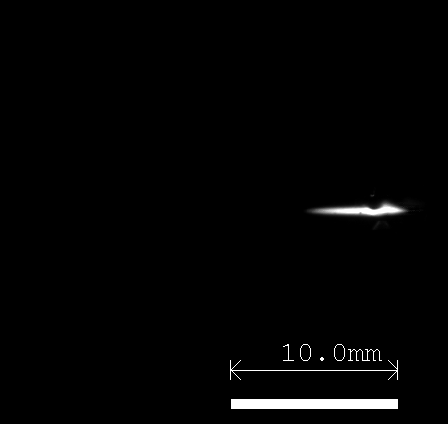
\includegraphics[width=\textwidth]{assets/4 experiments/V1 Spark Ignition Frames/LSP142_SPRK15_Fr33.bmp}
        \caption{\qty{3.3}{ms}}
        %\label{fig:ignition_frames_17}
    \end{subfigure}
    \hfill
    \begin{subfigure}[t]{0.3\textwidth}
        \centering
        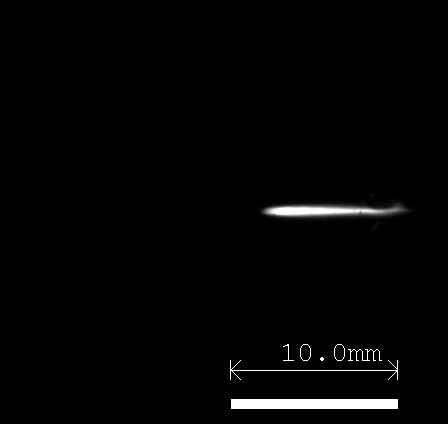
\includegraphics[width=\textwidth]{assets/4 experiments/V1 Spark Ignition Frames/LSP142_SPRK15_Fr35.bmp}
        \caption{\qty{3.5}{ms}}
        %\label{fig:ignition_frames_18}
    \end{subfigure}
    \begin{subfigure}[t]{0.3\textwidth}
        \centering
        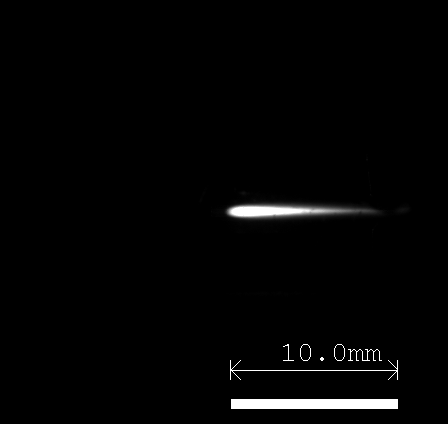
\includegraphics[width=\textwidth]{assets/4 experiments/V1 Spark Ignition Frames/LSP142_SPRK15_Fr38.bmp}
        \caption{\qty{3.8}{ms}}
        %\label{fig:ignition_frames_19}
    \end{subfigure}
    \hfill
    \begin{subfigure}[t]{0.3\textwidth}
        \centering
        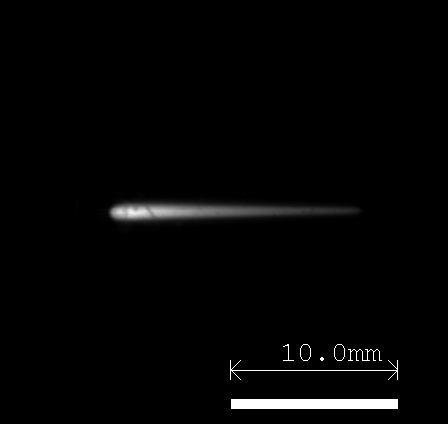
\includegraphics[width=\textwidth]{assets/4 experiments/V1 Spark Ignition Frames/LSP142_SPRK15_Fr69.bmp}
        \caption{\qty{6.9}{ms}}
        %\label{fig:ignition_frames_20}
    \end{subfigure}
    \hfill
    \begin{subfigure}[t]{0.3\textwidth}
        \centering
        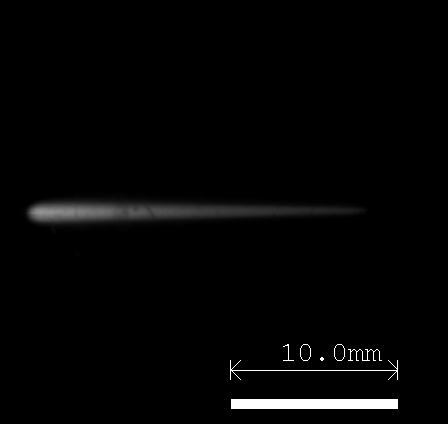
\includegraphics[width=\textwidth]{assets/4 experiments/V1 Spark Ignition Frames/LSP142_SPRK15_Fr130.bmp}
        \caption{\qty{13.0}{ms}}
        %\label{fig:ignition_frames_21}
    \end{subfigure}
    \caption{LSP spark initiation: \qty{3080}{W}, \qty{20}{bar}. \shotsettings{LSP142\_SPRK15}{0.1?? CHANGE}{22}{2048}}
    \label{fig:V1_spark_initiation_frames}
\end{figure}

            Selected frames of an entire LSP lifetime are shown in \autoref{fig:growth_frames}. The initially rapid LSP growth ($\sim$\qty{9}{m.s^{-1}}) slows down as it approaches steady conditions, with the front speed decreasing to less than \qty{1}{m.s^{-1}} by the end of the laser pulse. Steady-state conditions have thus not been truly achieved with full-power, \qty{10}{ms} pulses. The LSP responded practically instantaneously to the end of the laser pulse, as it dissipated from the the high speed footage in the span of 1--2 frames.
            
            \begin{figure}[h]
    \centering
    \begin{subfigure}[t]{0.47\textwidth}
        \centering
        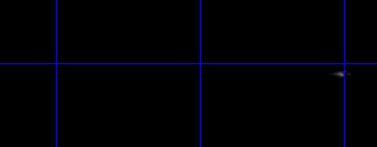
\includegraphics[width=\textwidth]{assets/5 results/1msFrames/16.jpg}
        \caption{\qty{1.6}{ms}}
        \label{fig:growth_frames_16}
    \end{subfigure}
    \hfill
    \begin{subfigure}[t]{0.47\textwidth}
        \centering
        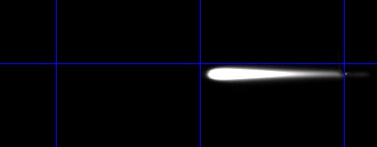
\includegraphics[width=\textwidth]{assets/5 results/1msFrames/26.jpg}
        \caption{\qty{2.6}{ms}}
        \label{fig:growth_frames_26}
    \end{subfigure}
    \hfill
    \begin{subfigure}[t]{0.47\textwidth}
        \centering
        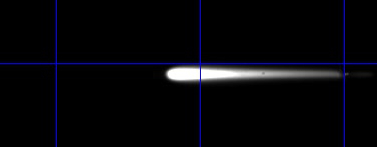
\includegraphics[width=\textwidth]{assets/5 results/1msFrames/36.jpg}
        \caption{\qty{3.6}{ms}}
        \label{fig:growth_frames_36}
    \end{subfigure}
    \hfill
    \begin{subfigure}[t]{0.47\textwidth}
        \centering
        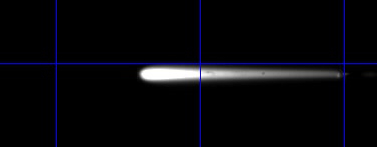
\includegraphics[width=\textwidth]{assets/5 results/1msFrames/46.jpg}
        \caption{\qty{4.6}{ms}}
        \label{fig:growth_frames_46}
    \end{subfigure}
    \hfill
    \begin{subfigure}[t]{0.47\textwidth}
        \centering
        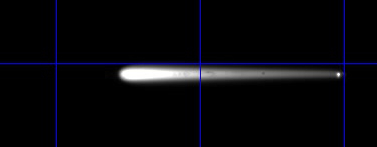
\includegraphics[width=\textwidth]{assets/5 results/1msFrames/56.jpg}
        \caption{\qty{5.6}{ms}}
        \label{fig:growth_frames_56}
    \end{subfigure}
    \hfill
    \begin{subfigure}[t]{0.47\textwidth}
        \centering
        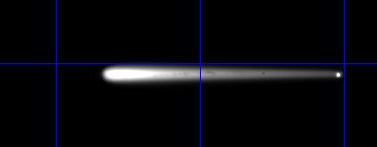
\includegraphics[width=\textwidth]{assets/5 results/1msFrames/66.jpg}
        \caption{\qty{6.6}{ms}}
        \label{fig:growth_frames_66}
    \end{subfigure}
    \hfill
    \begin{subfigure}[t]{0.47\textwidth}
        \centering
        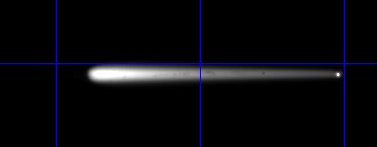
\includegraphics[width=\textwidth]{assets/5 results/1msFrames/76.jpg}
        \caption{\qty{7.6}{ms}}
        \label{fig:growth_frames_76}
    \end{subfigure}
    \hfill
    \begin{subfigure}[t]{0.47\textwidth}
        \centering
        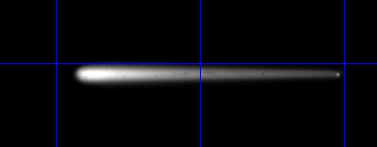
\includegraphics[width=\textwidth]{assets/5 results/1msFrames/86.jpg}
        \caption{\qty{8.6}{ms}}
        \label{fig:growth_frames_86}
    \end{subfigure}
    \hfill
    \begin{subfigure}[t]{0.47\textwidth}
        \centering
        \includegraphics[width=\textwidth]{assets/5 results/1msFrames/96.jpg}
        \caption{\qty{9.6}{ms}}
        \label{fig:growth_frames_96}
    \end{subfigure}
    \hfill
    \begin{subfigure}[t]{0.47\textwidth}
        \centering
        \includegraphics[width=\textwidth]{assets/5 results/1msFrames/106.jpg}
        \caption{\qty{10.6}{ms}}
        \label{fig:growth_frames_106}
    \end{subfigure}
    \hfill
    \begin{subfigure}[t]{0.47\textwidth}
        \centering
        \includegraphics[width=\textwidth]{assets/5 results/1msFrames/116.jpg}
        \caption{\qty{11.6}{ms}}
        \label{fig:growth_frames_116}
    \end{subfigure}
    \caption[LSP growth throughout 10-ms-laser pulse]{LSP growth throughout 10-ms-laser pulse: \qty{3080}{W}, \qty{20.29}{bar}. The blue grid is spaced by \qty{10}{mm}. \shotsettings{LSP1\_PS1}{0.1}{22}{2048}}
    \label{fig:growth_frames}
\end{figure}
    \clearpage
    \section{Power threshold} \label{sec:results_powerthreshold}
        Once LSP ignition had been confirmed, work began on reproducing power threshold experiments, a frequent topic in LSP research. The aim of this experiment is to determine the minimum laser power required to sustain a steady plasma, at a given pressure. Knowing this power threshold is useful to establish the operation bounds of an LSP facility, whether it is a laboratory experiment or a laser-thermal thruster. Several of such experiments have been performed for Argon with fiber-lasers: the work of \textcite{zimakovInteractionNearIRLaser2016, matsuiGeneratingConditionsArgon2019,luCharacteristicDiagnosticsLaserStabilized2022} will thus be used for comparison.
        
        \subsection{Methodology}
            The test section would be pressurized with Argon to a desired pressure between 3 and 20~bar. Then, determining the power threshold was done through a process akin to a binary search or bisection root-finding algorithm in computer science: LSP would be ignited first at the maximum setpoint power to confirm that the laser and igniter were aligned such that LSP was achievable. Power would then be reduced to a point far below the threshold (10~\% power) to confirm that LSP was not achieved. This brackets the threshold point. Subsequent tests would be performed at a power setpoint in the middle of this iteratively shrinking bracket, until the threshold was determined to be within approximately \qty{50}{W} below the last successful LSP test.

            This series of tests were performed with both spark and wire ignition. One issue encountered with wire ignition was that while lower laser powers could theoretically sustain LSP, they would not necessarily be sufficient to ignite it. To circumvent this issue, stepped laser pulse profiles were used instead of constant laser power. An example of such a pulse is shown in \autoref{fig:pulse_stepProfile}: the pulse begins at 100~\% setpoint power for \qty{0.5}{ms} to initiate the LSP off of the Tungsten wire. The power would then be stepped down to the desired power level, which would be maintained for as long as possible to ensure that the LSP could re-adjust to steady conditions.

            \begin{figure}[h]
                \centering
                \includegraphics[]{assets/5 results/pulse_profile}
                \caption[Typical stepped-pulse profile: \texttt{05L33\_15}]{Typical stepped-pulse profile: \texttt{05L33\_15}. A complete list of stepped-pulse specifications can be found in \autoref{chp:app_pulseShapes}.}
                \label{fig:pulse_stepProfile}
            \end{figure}

            Whether LSP could be considered steady for a given test was determined by observing its behavior in the high-speed footage. It needed to fulfill two conditions:
            \begin{enumerate}
                \item The LSP is still visible at the end of the laser pulse
                \item The LSP is not visibly changing by the time the laser pulse ended, i.e., it is not shrinking or dimming significantly.
            \end{enumerate}
            As plasma brightness changed with laser power, the variable ND filter would be adjusted to determine whether a vanishing plasma was unstable or simply too dim to be picked up through the lens filters.

        \subsection{Results}
            The resulting power threshold plot can be seen in \autoref{fig:powerthreshold}. Both spark and wire ignition experiments are shown, along with data reported by \textcite{zimakovInteractionNearIRLaser2016,matsuiGeneratingConditionsArgon2019,luCharacteristicDiagnosticsLaserStabilized2022}. The use of wire ignition shows a significant improvement in the minimum power required to sustain LSP over the spark ignition method. The improved reliability and ease of alignment afforded by wire ignition enabled sustaining LSP down to hundreds of Watts, whereas spark ignition struggled to ignite and sustain LSP below \qty{1}{kW}. Note that the uncertainties indicated on the wire ignition data reflect the possible range in which the true power threshold lies, and is not related to an uncertainty in the power measurement. \textcite{zimakovInteractionNearIRLaser2016} presented a model based on balancing input power with heat conduction ($P_\mathrm{h}$) and radiative losses ($P_\mathrm{r}$), to evaluate the power threshold as a function of pressure $P_\mathrm{t}$. This expression is reproduced here as \autoref{eq:zimakov_threshold}:
            \begin{equation} \label{eq:zimakov_threshold}
                P_\mathrm{t} = P_\mathrm{h} + P_\mathrm{r}
            \end{equation}
            \citeauthor{zimakovInteractionNearIRLaser2016}'s experiments had experimentally estimated the parameters of this equation for Argon as $p^2P_\mathrm{h} =$~\qty{26}{bar^2.kW} and $P_\mathrm{r} =$~\qty{240}{W}. This same model was fitted to this study's wire-ignited LSP data, yielding the following power threshold parameters: $p^2P_\mathrm{h} =$~\qty{11}{bar^2.kW} and $P_\mathrm{r} =$~\qty{178}{W}. These values can interpreted, respectively, as the minimum laser power to sustain LSP at \qty{1}{bar}, and the limiting laser power under which no LSP can be sustained even at high pressures.

            The discrepancy in the power thresholds achieved across different experiments is due in part to the optical quality of the focused beam, as suggested by \textcite{luCharacteristicDiagnosticsLaserStabilized2022}, who have so far achieved the best power-threshold results for fiber-laser-sustained Argon plasma. As the literature data is all from spark-ignited experiments, direct comparisons to wire ignition tests may be limited. However, this suggests that a low power threshold can be readily achieved by a basic optical train and a simple wire-ignition system combined with stepped pulse profiles, competing with methodologies that require far greater precision and optical quality.

            Qualitative observations were made on the LSP's response to the step-down in laser power. As seen in \autoref{fig:lsp_stepdown}, the decrease in input power is immediately apparent, with the plasma shrinking and dimming as soon as the power is dropped. The LSP re-adjusts to new power conditions in less than a millisecond. In this particular case, the LSP remained stable until the end of the laser pulse, \qty{14.8}{ms} after the step-down in power.


            \begin{figure}[h]
                \centering
                \includegraphics[]{assets/5 results/powerthreshold}
                \caption[Pressure-Power LSP threshold exploration]{Pressure-Power LSP threshold exploration. \textcite{zimakovInteractionNearIRLaser2016}'s model is fitted to wire ignition data as the blue dashed line.}
                \label{fig:powerthreshold}
            \end{figure}

            \begin{figure}[h]
                \centering
                \begin{subfigure}[t]{0.32\textwidth}
                    \centering
                    \includegraphics[trim=7.6in 5.3in 2.4in 5.5in, clip, width=\textwidth]{assets/5 results/LSP34_PS28/20.jpg}
                    \caption{\qty{2.0}{ms}, before step-down}
                    \label{fig:lsp_stepdown_20}
                \end{subfigure}
                \hfill
                \begin{subfigure}[t]{0.32\textwidth}
                    \centering
                    \includegraphics[trim=7.6in 5.3in 2.4in 5.5in, clip, width=\textwidth]{assets/5 results/LSP34_PS28/21.jpg}
                    \caption{\qty{2.1}{ms}, after step-down}
                    \label{fig:lsp_stepdown_21}
                \end{subfigure}
                \hfill
                \begin{subfigure}[t]{0.32\textwidth}
                    \centering
                    \includegraphics[trim=7.6in 5.3in 2.4in 5.5in, clip, width=\textwidth]{assets/5 results/LSP34_PS28/28.jpg}
                    \caption{\qty{2.8}{ms}, steady-state}
                    \label{fig:lsp_stepdown_28}
                \end{subfigure}
                \caption[LSP adjusting to step-down in power]{LSP adjusting to step-down in power, from 100~\% to 8.5~\% (\qty{255}{W}). \shotsettings{LSP34\_PS28}{0.1}{4}{2048}, pulse profile: \texttt{05L8.5\_15}, pressure: \qty{10.23}{bar}}
                \label{fig:lsp_stepdown}
            \end{figure}

    \clearpage
    \section{Laser Absorption} \label{sec:exp_absorption}
        Despite the reliability issues of spark ignition, LSP absorption data was successfully acquired at various pressures and laser pulse energies. Incomplete absorption of the incident laser radiation by IB is one of the major sources of inefficient heat deposition, so quantifying this loss is important to control it, reduce it, and  eventually optimize an LTP thruster.
        
        \subsection{Methodology}
            The Gentec power meter recorded the incident pulse energy for a subset of spark-ignited LSPs. Unfortunately, due to this ignition system's reliability issues, discussed in \autoref{sec:ignitiontest}, a systematic exploration of the variation in absorption due to experimental parameters could not be performed. Nevertheless, some preliminary data was acquired, with some consistency observed at \qty{20}{bar} of pressure.

            Constant-power, \qty{10}{ms} laser pulses were focused into the test section to ignite LSP. As seen in \autoref{tab:expTimeline}, a buffer time of \qty{1}{ms} between the start of the pulse and the spark ignition was used to ensure that the spark was triggered while the laser was on. The laser absorption $a$ by the LSP was defined as follows:
            \begin{equation}
                a = 1-\frac{E_\tau}{E_\mathrm{in}}
            \end{equation}
            Where $E_\tau$ is the measured (transmitted) energy reaching the power meter and $E_\mathrm{in}$ is the pulse energy incident on the LSP. Both variables were determined by correcting both for the losses through the experiment optics (given in \autoref{tab:opticalLoss}) and the \qty{1}{ms} buffer time.

        \subsection{Results}
            Calculated LSP absorption is tabulated in \autoref{tab:LSP_absorption}. Though there are a few outliers, overall absorption appears to lie between 70~\% and 90~\%. This is visualized in \autoref{fig:absorption_ap}. Data for several tests performed at a nominal pressure of \qty{20}{bar} can be seen in \autoref{fig:absorption_20bar}, where a linear function was fitted to the data to determine an average absorption factor of 79~\%.

            \begin{table}[h]
\centering
\caption[LSP energy absorption data]{LSP energy absorption data. $p$ is the nominal pressure; $E_\mathrm{pulse}$, $E_\mathrm{in}$, $E_\tau$, and $E_a$ are the laser pulse energy, input energy, transmitted energy, and computed absorption of the LSP, respectively.}
\label{tab:LSP_absorption}
\begin{tabular}{@{}lrrrrr@{}}
\toprule
Shot ID & $p$ [bar] & $E_\mathrm{pulse}$ [J] & $E_\mathrm{in}$ [J] & $E_\tau$ [J] & $a$ [-] \\
\midrule
\verb|LSP210_SPX11| &     20.20 &                  30.80 &               27.56 &         5.81 &    0.79 \\
\verb|LSP211_SPX12| &     20.00 &                  30.80 &               27.56 &         6.16 &    0.78 \\
\verb|LSP212_SPX13| &     20.00 &                  18.48 &               16.53 &         4.95 &    0.70 \\
\verb|LSP213_SPX14| &     19.90 &                  12.32 &               11.02 &         1.41 &    0.87 \\
\verb|LSP215_SPX16| &     20.00 &                  30.80 &               27.56 &         5.15 &    0.81 \\
\verb|LSP216_SPX17| &      6.09 &                  30.80 &               27.56 &         8.62 &    0.69 \\
\verb|LSP217_SPX18| &     10.10 &                  20.54 &               18.38 &        14.80 &    0.19 \\
\verb|LSP219_SPX20| &     15.00 &                  10.16 &                9.09 &         7.83 &    0.14 \\
\bottomrule
\end{tabular}
\end{table}

            
            \begin{figure}[h]
                \centering
                \begin{subfigure}[t]{0.47\textwidth}
                    \centering
                    \includegraphics[width=\textwidth]{assets/5 results/absorption_ia}
                    \caption{Absorption across a range of pressure. Variable pulse energy and chamber pressure.}
                    \label{fig:absorption_ap}
                \end{subfigure}
                \hfill
                \begin{subfigure}[t]{0.47\textwidth}
                    \centering
                    \includegraphics[width=\textwidth]{assets/5 results/absorption_20bar}
                    \caption{Input energy vs. absorbed energy, calculation of absorption}
                    \label{fig:absorption_20bar}
                \end{subfigure}
                \caption{Estimated energy absorption of LSP, \qty{20}{bar}}
                \label{fig:LSP_absorption_data}
            \end{figure}

            Such absorption figures appear to be in agreement with LSP literature stating that most of the laser radiation can be absorbed by the LSP under the right conditions (\textcite{keeferLaserSustainedPlasmas1989}). However, much higher absorption was shown to be achievable under some conditions, such as forced convection (\textcite{fowlerIgnitionMaintenanceSubsonic1975}). For instance, experiments by \textcite{toyodaThrustPerformanceCW2002} show between 80~\% and 99~\% absorption depending on the working gas and experimental conditions.

            This absorption data can also be paired with LSP footage to approximate the absorption coefficient of the LSP. For instance, \autoref{fig:LSP205_SPX6} shows the length measurement of an LSP (\qty{10}{bar}, \qty{3080}{W}) to be \qty{22}{mm} at its fullest extent.

            \begin{figure}[h]
                \centering
                \includegraphics[width=\textwidth]{assets/5 results/LSP6_10.23_length.png}
                \caption[Length estimation of LSP]{Length estimation of LSP. \qty{10.23}{bar}, \qty{30.8}{J} pulse. \shotsettings{LSP205\_SPX6}{0.1}{11}{2048}}
                \label{fig:LSP205_SPX6}
            \end{figure}

            Considering the transmission of radiation through an absorbing medium using the Beer-Lambert law:
            \begin{equation} \label{eq:beerlambert}
                \frac{I(d)}{I_0} = e^{-\alpha d}
            \end{equation}
            By considering the energy transmission $E_\tau/E_\mathrm{in}$ to be equivalent to the left-hand side of \autoref{eq:beerlambert}, and approximating the path length $d$ as the LSP length, the absorption coefficient can be estimated as follows:
            \begin{equation}
                \alpha = \frac{\ln{(E_\tau/E_\mathrm{in})}}{-d}
            \end{equation}
            For \texttt{LSP205\_SPX6}, this evaluates to \qty{73}{m^{-1}}. This in fact appears to match the absorption coefficient calculations performed in \autoref{chp:models}. \autoref{fig:ib_coeff} predicts an absorption coefficient of \qty{67}{m^{-1}}, while the calculations of \textcite{matsuiGeneratingConditionsArgon2019} predict a value of \qty{58}{m^{-1}}. While not in perfect agreement with theory, this estimate does appear to provide a value on the same order as predicted by IB absorption models.

            As mentioned earlier, the reliability issues of the spark ignition system prevented the systematic study of LSP absorption characteristics. The $\alpha$ estimate above unfortunately cannot account for the changing absorption/transmission as the LSP grows, and assumes a path length based on the final LSP size. Performing absorption measurements under CW regime would improve the measure of $\alpha$ considerably, as measurements could be made once the LSP is fully developed and steady.

    \section{Heat deposition}
        To fulfill this project's second research objective, i.e., determining LSP heat deposition in the working gas, the change in pressure from initial conditions was monitored with a PCB Piezotronics pressure transducer. As discussed on page \pageref{sec:design_pressuresensor}, this would theoretically allow the estimation of heat deposition without the need to directly track the temperature of the gas, which would have been a major challenge for a millisecond-scale event.

        \subsection{Methodology}
            The pressure data was collected in parallel with other experiments, all ignited using a wire-ignition method. As seen in \autoref{fig:finalsetup_static}, the pressure transducer was integrated using an instrumentation plug on top of the test section, \qty{1.5}{in} downstream from the ignition point. The transducer's signal was then processed by a signal conditioner whose output was recorded on an oscilloscope, along with the laser's internal power meter reading. This allowed the synchronization of both the laser's power and the pressure in the test section.

            A sample pressure signal is provided in \autoref{fig:pressure_noise}. The oscilloscope data featured significant noise, which was filtered out with an infinite impulse response filter to facilitate analysis. Pressure data was acquired for a variety of initial pressures and laser power levels.

            \begin{figure}[h]
                \centering
                \begin{subfigure}[t]{0.47\textwidth}
                    \centering
                    \includegraphics[width=\textwidth]{assets/5 results/pressure_noise}
                    \caption{Typical pressure change during and after LSP at \qty{3080}{W}, \qty{20.29}{bar}}
                    \label{fig:pressure_noise}
                \end{subfigure}
                \hfill
                \begin{subfigure}[t]{0.47\textwidth}
                    \centering
                    \includegraphics[width=\textwidth]{assets/5 results/pressure_elim}
                    \caption{Pressure rise due to alternate heat transfer mechanisms}
                    \label{fig:pressure_elim}
                \end{subfigure}
                \caption{Denoising of pressure data and comparison to other sources of heat}
            \end{figure}

            
            To ensure that the resulting pressure rise was primarily caused by the LSP, two tests were performed to rule out the effects of other potential factors:
            \begin{enumerate}
                \item The laser directly incident on the test section walls could heat up the walls which would then heat up the gas
                \item The ignition wire heating up could transfer its heat to the surrounding gas.
            \end{enumerate}
            While either scenario does ultimately heat up the gas, neither mechanism reflects the ideal operation of a laser-thermal thruster, where the plasma itself should be the dominant heat source. To quantify these effects, the following tests were performed at an initial pressure of \qty{10}{bar} and the resulting pressure rise was recorded:
            \begin{enumerate}
                \item The laser (\qty{10}{ms}, 100~\%) was pointed into an empty test section, such that the laser would be directly incident on an opaque backplate.
                \item A constant 20~\%, \qty{19.8}{ms} pulse (equivalent in energy to a \texttt{1L20\_15} stepped pulse) was focused on the ignition wire. The low constant power pulse is necessary to avoid igniting LSP.
            \end{enumerate}
            The pressure rise of these tests was then compared to that of a successful LSP at \qty{10}{bar}, sustained with a \texttt{1L20\_15} stepped pulse (\qty{12.1}{J}). This is shown in \autoref{fig:pressure_elim}. Some measurable effect on pressure is detected from both of these mechanisms, however, the pressure rise from LSP is greater by a factor 3 compared to direct heating of the ignition wire. Furthermore, the tests mentioned above represent an absolute worst case scenario for the magnitude of these heat transfer mechanisms. Absorption measurements discussed in \autoref{sec:exp_absorption} show that the majority of the laser power is absorbed by the LSP. This leaves less power for heat transfer by wire or chamber wall heating. Heating via the chamber walls in particular is not expected to significantly contribute to overall heat transfer, as the ignition wire would absorb most of any laser power transmitted through the LSP, and direct irradiation had only a minor effect in the first place.

        \subsection{Results}
            The pressure rise seen in \autoref{fig:pressure_noise} exhibits features that were consistently observed at different initial pressures and different laser powers. Namely, the pressure appears to rise continuously while the laser and the LSP is active. As soon as the laser is off and the LSP is extinguished, a small drop in pressure is observed, which is then followed by another, higher rise in pressure. Once the pressure reaches a maximum, usually around \qty{40}{ms} after the end of the laser pulse, it decreases a at slower rate relative to the rise, as the gas loses heat through conduction with the chamber walls. Such a pressure variation is unlikely to be from traveling pressure waves: The speed of sound in Argon at \qty{20}{\degreeCelsius} is \qty{319}{mm.ms^{-1}}, i.e., the test section's length every millisecond, while the observed pressure variation occurs over several hundredths of a second. This suggests that the pressure change observed by the pressure transducer reflects that of the overall test section static pressure.

            \autoref{fig:pressure_pressures} shows the pressure variation for a range of initial nominal pressures. As mentioned earlier, the features of this pressure rise remain consistent with a local maximum reached at the end of the laser pulse (\qty{10}{ms}). The magnitude of the pressure change does not appear to be strongly affected by the initial pressure. Assuming an even distribution of heat added into a closed system, the resulting pressure change $\Delta p$ can be expressed using the ideal gas equation and the change in temperature $\Delta T$ caused by a constant volume heat addition $Q_\mathrm{in}$:
            \begin{gather*}
                \Delta pV = mR_\mathrm{g}\Delta T \\
                Q_\mathrm{in} = mc_V\Delta T \\
                \Delta p = \frac{R_\mathrm{g}Q_\mathrm{in}}{Vc_V}
            \end{gather*}
            The resulting change in pressure is independent of the gas mass, and therefore, independent of the initial pressure for a set volume. This however would only hold as long as the heat deposited in the gas $Q_\mathrm{in}$ is also independent on the initial pressure.

            \begin{figure}[h]
                \centering
                \includegraphics[]{assets/5 results/pressure_pressures}
                \caption{Effect of varying initial pressure on pressure rise resulting from LSP}
                \label{fig:pressure_pressures}
            \end{figure}

            \autoref{fig:pressure_powers} shows the effect of reducing the laser pulse energy on the resulting pressure rise. In this case, the peak pressure appears to be correlated with pulse energy, decreasing consistently with decreasing energy. Here again, the change from \qtyrange{20}{10}{bar} of initial pressure does not appear to have an effect on the resulting heat deposition. The intermediate peak in pressure appears to occur later for lower energy pulses, this is due in part to the longer pulse duration. Another feature of the lower energy pressure rises is a decrease in the rate of change of pressure during the pulse---there is a clear change as the pulse switched from the high setpoint for ignition, to the lower sustained setpoint.

            \begin{figure}[h]
                \centering
                \includegraphics[]{assets/5 results/pressure_powers}
                \caption{Effect of varying the laser pulse energy on the pressure rise resulting from LSP}
                \label{fig:pressure_powers}
            \end{figure}

            A first estimation of the heat deposited in the working gas can be made based on the pressure change, assuming that the observed maximum pressure reflects a state where the heat has been distributed throughout the test section. 
            \begin{equation}
                Q_\mathrm{in} = \frac{\Delta pVc_V}{R_\mathrm{g}}
            \end{equation}
            The heat deposition efficiency $\eta$ can then be calculated as the ratio $Q_\mathrm{in}/E_\mathrm{in}$, which captures the overall efficiency of converting the incident laser power on the LSP into heat remaining in the propellant. This would include losses from incomplete laser absorption by the LSP, along with heat lost in the form of radiation, which would heat the chamber walls without really affecting the gas temperature.

            The detailed results of such a calculation are shown for a single LSP test in \autoref{fig:pressure_annotated}.

            \begin{figure}[h]
                \centering
                \includegraphics[]{assets/5 results/pressure_an_LSP16_PS16}
                \caption[Detailed analysis of pressure rise profile]{Detailed analysis of pressure rise profile, \qty{3080}{W}, \qty{12.5}{bar}.}
                \label{fig:pressure_annotated}
            \end{figure}

            Repeating this efficiency calculation for several LSPs sustained at various pressures and pulse energies yields \autoref{fig:heatEfficiency}. Heat deposition efficiency is seen to be consistent at around 15~\%, regardless of laser power or gas pressure.

            \begin{figure}[h]
                \centering
                \includegraphics[]{assets/5 results/heatEfficiency}
                \caption[Heat deposition efficiency of LSP]{Heat deposition efficiency of LSP. Left: calculation at 20 and 10~bar; right: consistency across a range of pressures, for two different pulse energies}
                \label{fig:heatEfficiency}
            \end{figure}

            Though useful to estimate heat deposition, the even distribution of heat in the test section does not accurately reflect the actual processes taking place during LSP growth and shortly afterward. This simplifying assumption does not explain the intermediate rise in pressure followed by a short drop immediately after the end of the laser pulse.

            Finally, this simple method of determining heat deposition and its efficiency could be improved on in a few ways. First, replicating these experiments using (a more reliable) spark ignition system would likely mitigate any heat transfer (though already estimated to be small) occuring via the ignition system. This would also allow the LSP to extend downstream past the ignition point, which may have implications on both laser absorption and overall heat deposition. Second, heat transfer to the walls should be quantified to determine whether this would explain the observed pressure drop after the (global) maximum, and to correct, if deemed necessary, for heat transfer to the walls as the gas is heating up. These changes would likely improve the calculated heat deposition efficiency.
    
    \clearpage
    \section{Spectroscopic temperature measurement} \label{sec:results_spectroscopy}
        Spectral data was acquired for several LSP tests, at \qty{20}{bar} and \qty{10}{bar} and varying laser power settings. No collimator was mounted to the fiber termination, allowing the spectrometer to sample a relatively large field of view of the experiment, rather than a single point on the plasma. The sampling area was determined to be approximately \qty{4}{cm} in diameter at the location of the LSP. This simplified alignment procedures as some part of the LSP's emission was practically guaranteed to be captured by the fiber, and it was assumed that the emitted radiation from the hottest part of the plasma would dominate over that of cooler regions.

        \autoref{fig:spectrum_lines} shows the captured spectral data from an LSP at \qty{20}{bar} and \qty{3}{kW} of laser power. Ar~I emission lines are clearly visible and closely match the lines tabulated by NIST~\cite{kramidaNISTAtomicSpectra2022}. Continuum radiation and Ar~II emission lines are also seen in the \qtyrange{400}{600}{nm} region, exhibiting the same features seen in spectra captured by \textcite{luCharacteristicDiagnosticsLaserStabilized2022}. However, unlike \citeauthor{luCharacteristicDiagnosticsLaserStabilized2022}'s data, the captured spectrum shows a drastic difference between the intensity of continuum radiation compared to the Ar~I line emissions, almost by an order of magnitude.

        \begin{figure}[h]
            \centering
            \includegraphics[]{assets/5 results/spectrum_LSP50_X7_lines}
            \caption{Detection of Ar I emission lines in \texttt{LSP50\_X7}}
            \label{fig:spectrum_lines}
        \end{figure}

        \subsection{Boltzmann plot method}
            Temperature calculation can be performed from spectral data using the Boltzmann plot method, summarized by \textcite{ohnoValidityElectronTemperature2006} and discussed in further detail by \textcite{griemSpectroscopicTemperatureMeasurements1997}. The transition of an electron from an upper atomic energy level $k$ to a lower level $i$  generates an emission line at wavelength $\lambda_{ki}$ with transition probability $A_{ki}$ and degeneracy for level $k$ of $g_k$. The following equation can be derived to relate these parameters to plasma temperature $T$:
            \begin{equation} \label{eq:transition_energy}
                \frac{\epsilon_{ki}\lambda_{ki}}{A_{ki}g_k} = \frac{\hbar cn}{2 \mathcal{Z}(T)}\exp{\left(-\frac{E_k}{k_\mathrm{B}T}\right)}
            \end{equation}
            Where $c$ is the speed of light, $n$ is the atomic number density, and $\mathcal{Z}(T)$ is the partition function. $\epsilon_{ki}$ is the spectrally integrated emission line intensity. This equation can be linearized with respect to $E_k$ by taking the natural log of both sides:
            \begin{equation} \label{eq:boltzmannplot}
                \ln{\frac{\epsilon_{ki}\lambda_{ki}}{A_{ki}g_k}} = -\frac{E_k}{k_\mathrm{B}T} + \ln{\frac{\hbar cn}{2 \mathcal{Z}(T)}}
            \end{equation}
            The second term is a constant for a given temperature, so $E_k$ can be plotted against the left-hand side of \autoref{eq:boltzmannplot}, resulting (in theory) in a straight line with gradient $-1/k_\mathrm{B}T$. This can then be used to evaluate $T$. However, as noted by \textcite{volkerImportancePhysicalUnits2022}, $\epsilon_{ki}\lambda_{ki}/A_{ki}g_k$ is not dimensionless, and a measure of absolute emission intensity can only be done with appropriate spectrometer calibration, which was not done in this study. There are several methods to resolve these issues, including one that can be used with the relative spectrometry data of this project: This ratio can be normalized by using a reference transition, denoted with the subscript $r$:
            \begin{equation} \label{eq:reference_transition}
                \left[\frac{\epsilon_{ki}\lambda_{ki}}{A_{ki}g_k}\right]_\mathrm{r} = \frac{\hbar cn_\mathrm{r}}{2 \mathcal{Z}_\mathrm{r}(T)}\exp{\left(-\frac{E_k}{k_\mathrm{B}T}\right)_\mathrm{r}}
            \end{equation}
            Multiplying either side of the original equation by the reciprocal of the above, then linearizing, yields the following, with the constant term bundled as $C$:
            \begin{equation}
                \ln{\left(\frac{\epsilon_{ki}\lambda_{ki}}{A_{ki}g_k}\left[\frac{A_{ki}g_k}{\epsilon_{ki}\lambda_{ki}}\right]_\mathrm{r}\right)} = \frac{-E_k+[E_k]_\mathrm{r}}{k_\mathrm{B}T} + C
            \end{equation}
            This normalization enables a temperature to be determined using relative spectral data, as they are all compared to the same reference line in the spectrum. This manipulation has no effect on the gradient of the plot.

        \subsection{Temperature calculation}
            The acquired spectral data for LSP was processed to extract temperature data using the Boltzmann plot method discussed in the previous section. A subset of emission lines strong enough to be consistently observed for all tests, and well separated from other lines to facilitate identification and spectral integration were selected for this analysis. Relevant properties for these transitions were acquired from the NIST Atomic Spectra Database~\cite{kramidaNISTAtomicSpectra2022}, and are tabulated for the selected lines in \autoref{tab:ArI_transitions}. The emission coefficients $\epsilon_{ki}$ were computed by fitting a Voigt line profile to the measured spectral lines, and integration was performed on the fitted curve. The \qty{763.51}{nm} transition was used as the reference line.

            \begin{table}[h]
                \centering
                \caption[Ar I transitions used to generate Boltzmann plot]{Ar I transitions used to generate Boltzmann plot. $\lambda_{ki}$ is the transition wavelength, $g_k$ is the degeneracy of the energy level $k$, $A_{ki}$ the transition probability from level $k$ to $i$, $\Delta A_{ki}/A_{ki}$ is the relative uncertainty of $A_{ki}$, and $E_k$ is the energy of level $k$. Taken from \textcite{kramidaNISTAtomicSpectra2022}.}
                \label{tab:ArI_transitions}
                \begin{tabular}{@{}Srrr@{}}
                    \toprule
                    $\lambda_{ki}$ [nm] & $g_kA_{ki}$ [\unit{s^{-1}}] & $\Delta A_{ki}/A_{ki}$ [-] & $E_k$ [eV]  \\ \midrule
                    696.54         & \num{1.90E+07}                    & 0.07                       & 13.328 \\
                    706.72         & \num{1.90E+07}                    & 0.10                       & 13.302 \\
                    738.40         & \num{4.20E+07}                    & 0.10                       & 13.302 \\
                    763.51         & \num{1.22E+08}                    & 0.10                       & 13.172 \\
                    794.82         & \num{5.58E+07}                    & 0.10                       & 13.283 \\
                    826.45         & \num{4.59E+07}                    & 0.07                       & 13.328 \\ \bottomrule
                \end{tabular}
            \end{table}

            A sample Boltzmann plot generated from LSP with \qty{20.14}{bar} Argon at \qty{3.08}{kW} is shown in \autoref{fig:boltzmannplot}. It is immediately apparent that the data points are very loosely correlated, providing low confidence in the resulting temperature, which was calculated to be \qty{8000}{K}. This does not appear possible, as ionization calculations such as the ones done in \autoref{sec:models_absorption} suggest Argon is not in a plasma state at these temperatures, and that little to no free electrons are available to absorb radiation via inverse bremsstrahlung. Furthermore, the selection of a different set of transition lines result in major variations in the computed temperature, sometimes suggesting negative absolute temperatures (characterized by a positive slope on the plot).
            
            \begin{figure}[h]
                \centering
                \begin{subfigure}[t]{0.47\textwidth}
                    \centering
                    \includegraphics[width=\textwidth]{assets/5 results/spectrum_LSP50_X7_boltzmann}
                    \caption{\qty{20}{bar}, \texttt{LSP50\_X7}: $T \approx$ \qty{8000}{K}}
                    \label{fig:boltzmann_LSP50_X7}
                \end{subfigure}
                \hfill
                \begin{subfigure}[t]{0.47\textwidth}
                    \centering
                    \includegraphics[width=\textwidth]{assets/5 results/spectrum_LSP60_S9_boltzmann}
                    \caption{\qty{10}{bar}, \texttt{LSP60\_S9}: $T \approx$ \qty{5000}{K}}
                    \label{fig:boltzmann_LSP60_S9}
                \end{subfigure}
                \caption{Boltzmann plots of selected LSP sustained at \qty{3}{kW}}
                \label{fig:boltzmannplot}
            \end{figure}

            There may be several reasons for this poor accuracy. The first is that the upper energy levels $E_k$ of most Ar I emission lines are clustered near \qty{13.25}{eV}, providing a poor sampling range for a linear regression. This is often the case when considering the relative line intensities only for a given atom or ion, as pointed out by \textcite{griemSpectroscopicTemperatureMeasurements1997}: excitation energies are often clustered together. This could be improved in two ways: the \qty{750.39}{nm} transition of Ar I has an excitation energy of \qty{14.95}{eV}, significantly greater than the other transitions. However, its closeness to the \qty{751.47}{nm} transition requires more sophisticated processing to discriminate its emission contribution from that of its neighboring line. Alternatively, a line emission of Ar I could be compared to an Ar II line. This however requires knowledge of electron density, and a measure of Ar II emission lines. These lines are present in the experimental data, in the \qtyrange{400}{500}{nm} range, but are much fainter than the Ar I lines, far more clustered together, and blended into the continuum radiation of the plasma, making detection and integration difficult.

            Another possible factor for poor temperature results is that the spectrometer fiber sampled a relatively large area in the test section, and that contrary to the assumption made before this experiment, the emitted radiation of the hottest parts of the LSP do not dominate over colder areas, at least not for the emission lines.  \textcite{nassarInvestigationLasersustainedPlasma2012} used a collimator to sample the spectrum from specific points in the plasma and had better success in determining temperature. 
    
    \section{Flowing experiments}
        To inform the design and test of dedicated thruster prototypes, the test section of this study was also designed such that it could be configured for flowing/thruster operation, by replacing the downstream end of the system with a backplate featuring an NPT-threaded port onto which various small nozzles could be inserted. Both the effects of forced flow on LSP properties, and the resulting thrust were of interest. This configuration is illustrated in \autoref{fig:finalsetup_flowing}. Due to the use of an opaque nozzle module, the power meter could no longer be used for absorption measurements. The facility was fitted on a thrust stand to attempt to measure any changes in the thrust of the apparatus due to the LSP.

        \begin{figure}[h]
            \centering
            \includegraphics[width=0.85\textwidth]{assets/5 results/finalsetup_flowing}
            \caption{Flowing configuration of the test section}
            \label{fig:finalsetup_flowing}
        \end{figure}

        Flow rate was controlled by a delivery pressure set by a regulator and choked orifice nozzles of varying diameter, made by drilling out blank NPT plugs. The test section static pressure was set such that choking conditions could be guaranteed, i.e., the ambient pressure was lower than the sonic pressure. This allows the calculation of the mass flow rate using \autoref{eq:massflow}, with the nozzle throat diameter $D_\mathrm{t}$, stagnation pressure $p_0$, and stagnation temperature $T_0$. 
        \begin{equation} \label{eq:massflow}
            \dot{m} = \sqrt{\frac{\gamma}{R_\mathrm{g}}\left(\frac{2}{\gamma+1}\right)^\frac{\gamma+1}{\gamma-1}}\frac{\pi D_\mathrm{t}^2p_0}{4\sqrt{T_0}} = K_{\dot{m}}\frac{\pi D_\mathrm{t}^2p_0}{4\sqrt{T_0}}
        \end{equation}
        For the temperatures of interest in the overall flow (excluding the LSP), $K_{\dot{m}}$ for Argon is \qty{0.0504}{s.K^{1/2}.m^{-1}}. Assuming incompressible conditions in the test section, the bulk fluid velocity $v_\mathrm{c}$ can be determined from \autoref{eq:massflow} and conservation of mass, resulting in \autoref{eq:bulk_fluid_vel}, where $D_\mathrm{c}$ is the test section internal diameter (\qty{1.5}{in}).
        \begin{equation} \label{eq:bulk_fluid_vel}
            v_\mathrm{c} = K_{\dot{m}}\frac{D_\mathrm{t}^2}{D_\mathrm{c}^2}R_\mathrm{g}\sqrt{T_0}
        \end{equation}
        Relatively large nozzle sizes were used to force flow in the test sections at speeds on the same order as the LSP growth speed ($\sim$~\qty{10}{m.s^{-1}}), to determine the LSP could be modified or blown out by fast enough flows. This is relevant for the thrust chamber design of an LTP thruster, as this could place constraints on the chamber dimensions. Unfortunately, the maximum nozzle diameter was limited to about \qty{4}{mm}, as this was the feed system's internal diameter. Using larger nozzles would have resulted in choking at the inlet, capping the mass flow rate (and test section flow velocity). The available nozzles under this diameter provided a bulk flow velocity in the test section of 0.88, 1.15, and \qty{1.79}{m.s^{-1}}.

        \autoref{fig:flow_v_static} compares the LSP size between the static and flowing case. What is apparent is a noticeably slower growth of the LSP in the upstream direction, suggesting that the forced flow does affect LSP dynamics. The upstream tip of the flowing LSP settles closer to the ignition point than for the static LSP. Forced flow also appears to help the LSP sever the ignition wire, allowing it to extend further past the ignition point, which was not always the case in static conditions. While the overall length of the flowing LSP is longer, it may not be appropriate to compare it to the static case as the wire prevents downstream growth.

        \begin{figure}[h]
            \centering
            \includegraphics[]{assets/5 results/flow_static_lsp.jpg}
            \caption[Comparison of LSP under forced flow (top) and static LSP (bottom)]{Comparison of LSP under forced flow (top) and static LSP (bottom). \qty{10}{bar}, \qty{3080}{W}, the bulk flow velocity was \qty{1.8}{m.s^{-1}}}
            \label{fig:flow_v_static}
        \end{figure}

        Although bulk flow velocities capable of blowing out the LSP were not attained, LSP stability was observed to be susceptible to flow conditions. As seen in \autoref{sec:background_exp}, past LTP facilities such as those of \textcite{toyodaThrustPerformanceCW2002} had features to distribute flow evenly in the test section with little turbulence. This was not the case in this project, as the gas was injected from a single orifice a few inches upstream of the LSP, through the side of the test section rather than co-axially. This likely results in flow with significant, unsteady, rotational and/or radial velocity components by the time it reaches the LSP. Disturbances to the LSP were observed, such as dissipation before the end of the laser pulse, separation of one LSP into two cores, which could sometimes reconnect, and localized variations in plasma brightness during a laser pulse.

        \autoref{fig:flow_pressure} presents the acquired pressure data for some flowing tests, including heat deposition efficiency calculations. The pressure profile matches the same pattern observed in static conditions. Although the data suggests a slightly lower heat deposition compared to the static case, the sample size is small, and the flow velocities remain low, almost comparable to static conditions. Definite conclusions based on this limited data may thus be premature. Nevertheless, one noticeable and consistent difference between the static and flowing cases is the intermediate pressure maximum---it appears to be 40~\% greater than in the static case. 

        \begin{figure}[h]
            \centering
            \begin{subfigure}[t]{0.47\textwidth}
                \centering
                \includegraphics[width=\textwidth]{assets/5 results/flow_deltap}
                \caption{Pressure rise}
                \label{fig:flow_pressure_rise}
            \end{subfigure}
            \hfill
            \begin{subfigure}[t]{0.47\textwidth}
                \centering
                \includegraphics[width=\textwidth]{assets/5 results/flow_eta}
                \caption{Calculated heat deposition efficiency}
                \label{fig:flow_pressure_efficiency}
            \end{subfigure}
            \caption[Pressure change and heat deposition efficiency in flowing LSP]{Pressure change and heat deposition efficiency in flowing LSP. \qty{10}{bar}, \qty{30.6}{J} input energy.}
            \label{fig:flow_pressure}
        \end{figure}
    \chapter{Conclusion and further work}
    Already identified as an alternative to chemical propulsion in the 1970s, laser-thermal propulsion promises the high specific impulse and thrust necessary to unlock rapid transit in the solar system. Whether this promise can be achieved in practice and at scale is however yet to be seen. McGill University's Interstellar Flight Experimental Research Group hopes to revive practical research on LSP for propulsion applications, by attempting to replicate and move beyond some of the work done in the late 20\textsuperscript{th} century with the fiber-optic lasers considered for use in other directed-energy propulsion concepts such as interstellar lightsails and laser-electric propulsion. By contrast with more recent LSP research which focused on non-propulsion applications, this project aimed to study the thermal, heat deposition, and thrust characteristics of LSP.

    A brief review of LTP and LSP literature was provided. DEP and LTP concepts were discussed, including their advantages and drawbacks. Research on LSP was summarized, starting with the physics of inverse bremsstrahlung (i.e., the physical mechanism powering LSP) and moving on the models and observations made through an intense period of research between 1970 and 1990. Researchers at the time were considering the use of \ce{CO_2} lasers emitting \qty{10.6}{\um} radiation, and the implications of a switch to \num{1.06}-\unit{\um} fiber-optic lasers were mentioned: while the range of these lasers is an order of magnitude greater, the lower IB absorption coefficient at this wavelength mandates higher laser power and/or pressure to sustain LSP. The design of past LSP facilities was briefly reviewed to provide context for the design choices made in creating such a facility at McGill, for the purposes of studying heat deposition and resulting thrust characteristics of argon LSP.

    The design process of the LTP thruster laboratory model was then reported in detail. The system's design was driven in large part by the constraints set by the laser available for this experiment, capable of emitting \num{3}-\unit{kW} pulses, but only for \qty{10}{ms}. The reasoning behind the decision to retrofit existing apparatus instead of opting for a clean-sheet design was discussed at length: given the many practical uncertainties surrounding the system, and the short timeline available for this project, the retrofit of a perhaps unoptimized test section was deemed preferable to inform the future design of a dedicated thruster model. This came at the cost of hindering thrust experiments, but this tradeoff paid off with the lessons learned in designing and rapidly testing an ignition system, developing diagnostic methodologies, and actually performing LSP experiments.

    Some modelling work was performed as part of this thesis, mainly to gain an understanding of the physics involved in inverse bremsstrahlung and the relevant parameters driving laser-sustained plasma. Namely, chamber pressure is a key parameter of any thermal propulsion system, with high pressures providing greater thrust. In LTP, higher pressures are also beneficial to improve LSP absorption properties. Predicting peak absorption (with respect to temperature) is also helpful to estimate the maximum temperature reached in the LSP, as it has been found to be correlated. \added{A simple model for LSP sizing prediction based on deposited laser energy was discussed, yielding temperature and size estimates on the same order as reported in literature and observed in experiment, respectively. The effects of heat deposition in the test section are also modelled, providing the means to estimate the heat deposition efficiency of LSP from experimental measurements. The modelling effort ends with an analysis of the expected performance of an LTP thruster model, suggesting that a dedicated thruster prototype should exhibit significant changes in thrust and exhaust velocity when powered by a laser---as long as the mass-flow rate is lower than \qty{1}{g.s^{-1}}.}

    Finally, the first results of a series of experiments were reported. Preliminary ignition tests quickly revealed the challenges posed by spark ignition. The use of such a system when constrained by a short laser pulse requires careful design to consistently align the laser focus and the spark. Successful LSP ignition using this system was difficult, but was achieved a few times, enough to build a small dataset on the laser absorption ability of LSP, which was observed to range from 70 to 90\%. Initial estimates on the absorption coefficient, derived from the absorption data and high-speed footage, appear to agree with this study's modelling, although a more systematic absorption study would be needed to confirm this. For other experiments, wire ignition was found to be far more reliable than spark ignition and allowed the replication of power threshold studies done in other LSP literature, finding that this ignition system provides a competitively low power threshold without the need of high precision optics. Spectral data acquired during these experiments should theoretically provide a measure of peak plasma temperature, but there appears to be methodology and/or processing issues to be resolved to provide a realistic temperature estimate. Flowing experiments were performed to explore the impact of incoming flow on LSP properties, but the feed system limitations only allowed for a cursory exploration.
    
    The recorded pressure change during and shortly after the LSP provided an insight into the heat deposition into the gas volume by the LSP. This ability will be crucial in a fully realized LTP system: to provide specific impulse on the order of \qty{3000}{s} yet high thrust, the LSP is meant to heat the surrounding propellant, and not be exhausted by itself (which would result in higher specific impulse but only for low thrust). The experimental data suggests a low heat-deposition efficiency of around 15\%, relative to the laser power incident on the LSP. Combined with the measured absorption, this builds an overall picture of the major loss factors involved in LSP: incomplete laser absorption and heat radiated to the walls or outside the test section appear to be responsible for 20\% and 65\% of the energy losses, respectively. This provides a baseline on efficiency that can now be improved on with a variety of strategies suggested in the LTP literature. The peculiar shape of the pressure profile, with its local maximum and minimum, should be the subject of further study.

    The objectives set for this project, to build an argon LTP thruster model, may not have been entirely met. Issues encountered with the unoptimized test section and its impact on thrust measurement meant that meaningful thrust experiments could not be performed. However, a method to determine heat deposition into the working gas was developed based on the pressure change of the test section, providing a baseline on heat-deposition efficiency, which can be used to design the next iteration of an LTP thruster at McGill University. In this regard, the project is successful in initiating a new experimental research effort on LTP at the IFERG, and the questions and issues raised across various aspects of this project could motivate several new, more targeted studies.

    \section{Further work}
        As this thesis project's \emph{raison d'être} was to lay the groundwork for experimental research on LSP and LTP at McGill, there are many opportunities for further work. A selection of such opportunities is given below.

        \paragraph{Optimization of the test section} Although the retrofit of the cavitation experiment's test section enabled rapid experimentation, its non-optimal design posed several challenges, some of which were already discussed in \autoref{sec:design_testSection}. The test section mass was particularly problematic for thrust experiments. Further research on LSP and LTP will be limited without the development of a new LSP generator or prototype thruster optimized for this project. Such optimizations would include:
        \begin{itemize}
            \item Opting for a lighter material for the pressure vessel, likely aluminum, to minimize weight
            \item Reducing the overall length and diameter of the vessel. This would both provide more flexibility in terms of beam geometry, allowing the use of shorter lenses or placing the laser focus at different locations in the chamber, to potentially optimize the LSP location relative to the nozzle. Smaller dimensions would also reduce the overall weight\added{ and result in a greater measured change in temperature and pressure, as implied by \autoref{eq:heatdep}}.
            \item Smaller observation windows. Although the current side windows offer excellent visibility throughout the length of the test section, their slender geometry and length mandated the use of heavy steel mounting clamps. Opting for lighter, smaller round windows bolted directly into the pressure vessel's body may be sufficient.
        \end{itemize}
        Such improvements would greatly facilitate the development of an appropriate thrust stand and provide greater beam-shaping flexibility without compromising on laser absorption measurements.

        \paragraph{Improved spark-ignition system} As discussed in \autoref{sec:ignitiontest}, the original spark-igniter design for this study proved difficult to work with, as the large spark gap and side-by-side electrodes created inconsistent arc paths that would rarely intersect with the laser beam path. Although good results were obtained with wire ignition, spark ignition is still thought to be optimal for future experiments, as its advantages over wire ignition would be worth the additional development efforts. As a reminder, they are as follows:
        \begin{itemize}
            \item An uninterrupted laser beam path allows determining the absorbed laser power and the absorption coefficient. It also does not impede the downstream growth of the LSP.
            \item Sparks can be generated at will without consuming material between each test. Several experiments could potentially be done in quick succession without re-aligning optics or replacing the ignition wire.
        \end{itemize}
        In order to improve spark consistency and ignition reliability, several improvements could be made to both the spark-plug design and how it integrates in the test section:
        \begin{itemize}
            \item The electrodes should be in a co-axial configuration, as was done for several LSP experiments in the literature (\textcite{luCharacteristicDiagnosticsLaserStabilized2022, zimakovInteractionNearIRLaser2016,matsuiGeneratingConditionsArgon2019}). This may improve the consistency of the arc path and would enable precise mechanical control of electrode distance more easily than with side-by-side electrodes.
            \item To accommodate for such an electrode arrangement, the test section should be modified with instrumentation ports along the opposite wall of the cylinder. Each port should ideally be precisely matched with another port facing it.
            \item Electrode tip distance should be reduced down to about a millimeter to favor arcing even at \qty{20}{bar} and to constraint possible arc paths to those intersecting with the laser focus. Ideally, this gap should be adjustable in order to adapt the electrode distance based on the test pressure.
            \item Discussions with researchers experienced with spark igniters suggested that a sharp tipped electrode paired with a rounded electrode gave better results.
        \end{itemize}

        \paragraph{Specific impulse measurement} One of the ultimate goals of the LTP project at McGill University is to demonstrate the feasibility of the concept and show that a specific impulse of \qtyrange{1000}{3000}{s} is possible under the right conditions. While the roadmap to this sort of performance is long and would involve a switch to hydrogen as a working gas, the experiment should be set-up such that mass-flow rates can be controlled and/or measured, enabling the calculation of exhaust velocity when combined with thrust data. This can be done using a mass flowmeter or by controlling mass flow by operating the facility in a double-choked configuration (choked at inlet and exhaust nozzle).

        \paragraph{Absorption measurements in flowing conditions} The nozzles used in this study could be easily fabricated and swapped on the test section but made it impossible to acquire an accurate measure of the laser power transmitted through the LSP and out of the test section, as the orifice size was significantly smaller than the laser beam. Designing a nozzle module that allows such a measurement would permit the study of the effect of flow on laser absorption. Poor laser absorption is one of the main efficiency loss mechanisms for an LTP thruster, so being able to measure it in flowing conditions would be valuable. This can be done either by using a regular laser window mount with an off-axis nozzle, or by designing an annular nozzle around the laser window (whether this option is worth the considerable design effort is debatable).

        \paragraph{Additional spectrometry and thermal imaging} As discussed in \autoref{sec:results_spectroscopy}, there is much room to improve this experiment's spectroscopy methodologies. The spectrometer's fiber termination should be equipped with a collimator to sample precise points in the LSP, which should improve the spectral data for temperature estimation with the Boltzmann plot method. Once this is corrected, the collimator could be mounted on opto-mechanical stages to precisely position it relative to the LSP, enabling the construction of temperature maps of the LSP, which could be compared to axisymmetric numerical models currently in development at McGill (\textcite{baoTwoDimensionalSimulationLasera}). In addition to spectroscopy, infrared thermal imaging could potentially be used to study the change in temperature of the cooler surrounding gas, providing additional data on the effective heat deposition from the LSP.
    
    \clearpage
    \defbibnote{bibmark}{\markright{}}
    \printbibliography[
        heading=bibintoc,
        title={References},
        block=ragged,
        prenote=bibmark
        ]
    \newpage

    \appendix
    \newcommand{\footeronly}{\thispagestyle{fancy}\markboth{}{}}
    \chapter{YLR-300/3000-QCW-MM-AC calibration report}
        \label{chp:app_YLR}
        \includepdf[pages=-, pagecommand={\footeronly}]{assets/appendices/IPGLaser300-3000_calib.pdf}
    \chapter{P30 collimator calibration report}
        \label{chp:app_Collimator}
        \includepdf[pages=-, pagecommand={\footeronly}]{assets/appendices/D30_Collimator_calib.pdf}
    \chapter{Test section apparatus drawings}
        The test section used in this thesis was originally designed to study the onset of cavitation in piston-cylinder assemblies. These drawings were drafted by John Kokkalis at McGill University, reproduced here with his permission. Although the apparatus represented here was not the iteration used in his final work, the final iteration of this system can be found in his Master's thesis~\cite{kokkalisOnsetCavitationDynamically2023}.
        \label{chp:app_CavitatorDrawings}
        \includepdf[pages=-, landscape=true, pagecommand={\thispagestyle{fancy}}]{assets/appendices/FULL_DRAWINGS_V4.pdf}
    \chapter{Laser window mount drawings}
        \label{chp:app_lwmDrawings}
        \includepdf[pages=-, landscape=true, pagecommand={\thispagestyle{fancy}}]{assets/appendices/LWM_allDrawings.pdf}
        \includepdf[landscape=true, pagecommand={\thispagestyle{fancy}\label{chp:app_optics}}]{assets/appendices/optics_diagram.pdf}
    \chapter{Instrumentation datasheets and calibration reports}
        \label{chp:app_calibration}
        \includepdf[pages={1}, pagecommand={\thispagestyle{fancy}\label{ds:laserPM}}]{assets/appendices/Gentec-EO_UP55N_PowerMeter_Calibration.pdf}
        \includepdf[pages={2}, pagecommand={\thispagestyle{fancy}}]{assets/appendices/Gentec-EO_UP55N_PowerMeter_Calibration.pdf}
        \includepdf[pages=-, pagecommand={\thispagestyle{fancy}\label{ds:pcbPressure}}]{assets/appendices/Calibration-Certificate_113B28-LW41871.pdf}
    \newcommand{\calculation}[3]{
    \begin{multline*}
        #1 = #2 \\ #1 = #3
    \end{multline*}
}

\chapter{Calculation examples} \label{chp:app_calc_ex}
    \section{Absorption coefficient} \label{sec:app_calc_ex_alpha}
        Calculation of the absorption coefficient $\alpha$ of an argon plasma for 1070-nm radiation at a temperature $T$ of \qty{15000}{K} and a pressure $p$ of \qty{10}{bar}.

        \subsection*{Givens}
            \begin{tabular}{r@{ = }l}
                $E_\text{ion}$      & \qty{15.76}{eV} \\
                $p$                 & \qty{10e+5}{Pa} \\
                $T$                 & \qty{15000}{K}  \\
                $\lambda$           & \qty{1.07e-6}{m}
            \end{tabular}
            \newcommand{\evalp}{\qty{10e+5}{Pa}}
            \newcommand{\evalT}{\qty{15000}{K}}

        \subsection{Electron density calculation}
            We begin with the calculation of electron density $n_\mathrm{e}$, using the Saha ionization equation:
            \begin{equation*}
                \frac{n_\mathrm{e}^2}{n_0-n_\mathrm{e}} = \frac{n_\mathrm{e}^2}{n_\mathrm{Ar}} = \frac{2}{\Lambda_\mathrm{th}^3}\frac{\mathcal{Z}_{\mathrm{Ar}^+}}{\mathcal{Z}_\mathrm{Ar}}\exp{\left(-\frac{E_\text{ion, Ar}}{k_\mathrm{B}T}\right)}
                \tag{\ref{eq:saha} revisited}
            \end{equation*}
            Calculating necessary parameters: the thermal DeBroglie wavelength $\Lambda_\mathrm{th}$, the initial atomic number density $n_0$, the partition function ratio $\mathcal{Z}_{\mathrm{Ar}^+}/\mathcal{Z}_\mathrm{Ar}$ (from NIST), and the ionization energy $E_\text{ion}$ in J.
            \begin{multline*}
                \Lambda_\mathrm{th} = \sqrt{\frac{2\pi\hbar^2}{m_\mathrm{e}k_\mathrm{B}T}} = \sqrt{\frac{2\pi(\evalhbar)^2}{(\evalme)(\evalkB)(\evalT)}} \\
                \Lambda_\mathrm{th} = \qty{6.0860e-10}{m}
            \end{multline*}
            \begin{multline*}
                n_0 = \frac{N_\mathrm{A}p}{R_\mathrm{u}T} = \frac{(\evalNA)(\evalp)}{(\evalRu)(\evalT)} \\
                n_0 = \qty{4.8286e24}{m^{-3}}
            \end{multline*}
            \begin{multline*}
                \frac{\mathcal{Z}_{\mathrm{Ar}^+}}{\mathcal{Z}_\mathrm{Ar}} = \frac{(5.74)}{(1.02)} \\ 
                \frac{\mathcal{Z}_{\mathrm{Ar}^+}}{\mathcal{Z}_\mathrm{Ar}} = 5.627
            \end{multline*}
            \calculation{E_\mathrm{ion}}{
                (\qty{15.76}{eV})\left(\frac{\qty{1.60218e-19}{J}}{\qty{1}{eV}}\right)
            }{
                \qty{2.5250e-18}{J}
            }
            Evaluating \autoref{eq:saha} with the above parameters then yields the ratio $n_\mathrm{e}^2/(n_0-n_\mathrm{e})$, which will be represented by $S$ for convenience:
            \calculation{\frac{n_\mathrm{e}^2}{n_0-n_\mathrm{e}} = S}{
                \frac{2(5.627)}{(\qty{6.0860e-10}{m})^3}\exp{\left(-\frac{(\qty{2.5250e-18}{J})}{(\evalkB)(\evalT)}\right)}
            }{
                \qty{2.5308e23}{m^{-3}}
            }
            The electron density can then be determined by solving  the quadratic equation:
            \begin{equation*}
                \frac{n_\mathrm{e}^2}{n_0-n_\mathrm{e}} = S \implies n_\mathrm{e}^2+Sn_\mathrm{e}-Sn_0 = 0
            \end{equation*}
            \calculation{n_\mathrm{e}}{
                \frac{-S+\sqrt{S^2-4(-Sn_0)}}{2}
            }{
                \qty{9.8612e23}{m^{-3}} = \qty{9.8612e17}{cm^{-3}}
            }

        \subsection{Absorption coefficient}
            For convenience, the IB absorption coefficient $\alpha$ formula is reproduced here, yielding a result in \unit{m^{-1}}:
            \begin{equation*}
                \ibalphaeq \tag{\ref{eq:ib_absorption} revisited}
            \end{equation*}
            It should be noted, again, that this form of the absorption coefficient expression is only valid with $n_\mathrm{e}$ in \unit{cm^{-3}} and $k_\mathrm{B}T_\mathrm{e}$ in \unit{eV} (i.e., \qty{1.293}{eV}). The Coulomb logarithm can be computed first---both approaches discussed in \autoref{sec:models_absorption} will be performed to compare their results. First is the following approximation, with $n_\mathrm{e}$ [\unit{cm^{-3}}] and $T_\mathrm{e}$ [eV]:
            \calculation{\ln{\Lambda}}{
                23 - \ln{(n_\mathrm{e}^{1/2}ZT_\mathrm{e}^{-3/2})}\\
                = 23 - \ln{((\qty{9.8612e17}{cm^{-3}})^{1/2}(1)(\qty{1.293}{eV})^{-3/2})}
            }{2.669}
            The alternate evaluation of the Coulomb logarithm is that of \textcite{johnstonCorrectValuesHighfrequency1973}:
            \begin{equation*}
                \ln{\Lambda} = \ln{\left(\frac{v_T}{\max{(\nu, \nu_\mathrm{p})}\rho_\mathrm{min}}\right)}
            \end{equation*}
            \calculation{v_T}{
                \sqrt{\frac{k_\mathrm{B}T}{m_\mathrm{e}}} = \sqrt{\frac{(\evalkB)(\qty{15000}{K})}{(\evalme)}}
            }{\qty{476800}{m.s^{-1}}}
            \autoref{fig:coulomb_freq} already showed that the laser frequency $\nu$ is much greater than the plasma frequency $\nu_\mathrm{p}$, but both will be compared here explicitly for completeness.
            \calculation{\nu}{\frac{c}{\lambda} = \frac{(\evalc)}{(\qty{1.07e-6}{m})}}{\qty{2.80e14}{s^{-1}}}
            \calculation{\nu_\mathrm{p}}{\frac{1}{2\pi}\sqrt{\frac{e^2}{\epsilon_0 m_\mathrm{e}}}\sqrt{n_\mathrm{e}} = (\qty{8978.85}{cm^{3/2}.s^{-1}})\sqrt{(\qty{9.8612e17}{cm^{-3}})}}{\qty{8.92e12}{s^{-1}}}
            \calculation{\max{(\nu, \nu_\mathrm{p})}}{\max((\qty{2.80e14}{s^{-1}}), (\qty{8.92e12}{s^{-1}}))}{\qty{2.80e14}{s^{-1}}}
            The minimum impact parameter $\rho_\mathrm{min}$ for electron--ion collisions is calculated as follows:
            \begin{equation*}
                \rho_\mathrm{min} = \max{\left(\frac{Ze^2}{k_\mathrm{B}T}, \frac{\hbar}{\sqrt{m_ek_\mathrm{B}T}}\right)}
            \end{equation*}
            \calculation{\frac{Ze^2}{k_\mathrm{B}T}}{
                \frac{(1)(\evale)^2}{(\evalkB)(\qty{15000}{K})}
            }{\qty{1.239e-19}{m}}
            \calculation{\frac{\hbar}{\sqrt{m_ek_\mathrm{B}T}}}{
                \frac{(\evalhbar)}{\sqrt{(\evalme)(\evalkB)(\qty{15000}{K})}}
            }{\qty{2.428e-10}{m}}
            \calculation{\rho_\mathrm{min}}{
                \max{\left(\frac{Ze^2}{k_\mathrm{B}T}, \frac{\hbar}{\sqrt{m_ek_\mathrm{B}T}}\right)} = \max{((\qty{1.239e-19}{m}),(\qty{2.428e-10}{m}))}
            }{\qty{2.428e-10}{m}}
            With this, the Coulomb logarithm evaluates to:
            \calculation{\ln{\Lambda}}{
                \ln{\left(\frac{v_T}{\max{(\nu, \nu_\mathrm{p})}\rho_\mathrm{min}}\right)} = \ln{\left(\frac{(\qty{476800}{m.s^{-1}})}{(\qty{2.80e14}{s^{-1}})(\qty{2.428e-10}{m})}\right)}
            }{1.948}
            Either approach for evaluating the logarithm can be taken. Although their result differs by 37\% in this case, the discrepancy decreases at higher temperatures, and the discrepancy's effect on the peak absorption coefficient is no greater than 10\% on both the temperature at which the peak occurs and the value of the peak. The absorption coefficient $\alpha$ can now be calculated:
            \begin{multline*}
                \alpha = \frac{7.8\times 10^{-7}Zn_\mathrm{e}^2\ln{\Lambda}}{\nu^2(k_\mathrm{B}T_\mathrm{e})^{3/2}} \left(1-\frac{\nu_\mathrm{p}^2}{\nu^2}\right)^{-1/2} \\
                = \frac{7.8\times 10^{-7}(1)(\qty{9.8612e17}{cm^{-3}})^2\ln{\Lambda}}{(\qty{2.80e14}{s^{-1}})^2(\qty{1.239}{eV})^{3/2}} \left(1-\frac{(\qty{8.92e12}{s^{-1}})^2}{(\qty{2.80e14}{s^{-1}})^2}\right)^{-1/2} \\
                = (\qty{7.019}{m^{-1}})\ln{\Lambda}\\
                \alpha = \biggl\{ \begin{array}{l}
                    \qty{18.7}{m^{-1}}\text{ for }\ln{\Lambda} = 2.669 \\
                    \qty{13.7}{m^{-1}}\text{ for }\ln{\Lambda} = 1.948 \\
                \end{array}
            \end{multline*}

    \chapter{LSP shot procedure} \label{chp:app_procedure}
        This procedure was published as a living document on a collaboration platform accessible to personnel associated with this project. It is reproduced here in its most up-to-date state at the time of publication.

        \newcommand{\warningsymbol}{\colorbox{Goldenrod}{\textbf{!}}}
\renewcommand{\warningsymbol}{\includegraphics[height=1.6ex]{assets/warning.png} }
\newcommand{\infosymbol}{\includegraphics[height=1.6ex]{assets/info.png} }
\newcommand{\stopsymbol}{\includegraphics[height=1.6ex]{assets/stop.png} }
\section*{LSP Shot Procedure}\label{lsp-shot-procedure}

This checklist is used for starting up, using, then shutting down the
Laser-Sustained Plasma (LSP) experiment to perform an LSP test. This
checklist assumes the laser has already been aligned.

Not all components are used for all experiments (e.g., spark-igniter).
Avoid setting them up if not necessary.

\subsubsection{STARTUP PROCEDURE}\label{startup-procedure}

\begin{enumerate}
\def\labelenumi{\arabic{enumi}.}

\item
  Power on triggering and monitoring station

  \begin{enumerate}
  \def\labelenumii{\arabic{enumii}.}
  
  \item
    Turn on delay generators, oscilloscope
  \item
    Oscilloscope trigger should be set to ``Normal'' mode
  \item
    Turn on laser in LOCAL mode
  \item
    Verify that timing delays have the correct value \textbf{and} unit
    (ms)
  \item
    Verify that delay generators, camera, and laser are connected
    according to wiring diagram
  \end{enumerate}
\item
  Setup camera

  \begin{enumerate}
  \def\labelenumii{\arabic{enumii}.}
  \item
    Turn on camera
  \item
    Connect to camera using Yellow Cat 6 cable
  \item
    Start PFV4 software and acquire live camera feed
  \item
    Calibrate sensor
  \item
    Remove lens cap
  \item
    Attach ND Filter and UV-IR Cut Filter to lens
  \item
    Adjust camera position and focus to frame the LSP ignition point
    (spark-plug tips) at a 300 mm focal length

    \infosymbol {\color{cyan} Use low-light mode, set the lens aperture to f/4, set the ND
    Filter to minimum, and use additional lighting if needed}
  \item
    Turn off low-light mode, set the camera frame rate to 10000 fps
  \item
    Set the aperture to f/22 and the ND filter to the maximum level
  \end{enumerate}
\item
  Setup power meter

  \begin{enumerate}
  \def\labelenumii{\arabic{enumii}.}
  \item
    The black rubber protective cap should be on
  \item
    Plug in the power meter's fan power supply and ensure the fan is
    running
  \item
    Turn on the BLU emitter (blue button)
  \item
    Connect to the power meter on the PC Gentec-EO software using the
    Bluetooth dongle (attached to blue USB extension cord)

    \infosymbol {\color{cyan} For best results, leave the Bluetooth dongle within the test area}
  \item
    Remove the black rubber protective cap and allow the power meter's
    signal to stabilize
  \item
    Set the wavelength to 1070 nm and perform the zeroing procedure
  \item
    Set the power meter to ``SSE (J)'' (Single Shot Energy) mode
  \item
    Suggested: set the display mode to ``Statistics''
  \item
    If applicable, set your acquisition settings (filename, etc.)
  \end{enumerate}
\item
  Setup spectrometer

  \begin{enumerate}
  \def\labelenumii{\arabic{enumii}.}
  
  \item
    Use a laser pointer and a 100 micron fiber attached to the fiber
    mount to ensure the fiber tip is pointed at the ignition point, then
    re-attach the spectrometer fiber (10 micron) to the fiber mount
  \item
    Connect to the spectrometer via USB and start the OceanView Lite
    software, in ``Quick View'' mode
  \item
    Click ``Create dark background spectrum''
  \item
    Set the integration time to 4 ms and the trigger mode to ``Edge''
  \end{enumerate}
\item
  Setup pressure transducer

  \begin{enumerate}
  \def\labelenumii{\arabic{enumii}.}
  
  \item
    If the transducer is already mounted, all that is needed is to turn
    on the signal conditioner and check that the Channel 1 indicator is
    green
  \end{enumerate}
\item
  Prepare test area

  \begin{enumerate}
  \def\labelenumii{\arabic{enumii}.}
  \item
    Ensure the laser protection panels (2) are installed over the beam
    path between the collimator and the test section
  \item
    Ensure that the collimator cap is \textbf{OFF}
    and no obstacle is present in the beam path. Use the guide laser to
    check.
  \item
    Pressurize the test section to the target pressure. If performing a
    flowing test, pressurize the feed lines upstream of the solenoid
    valve, and set the valve's safety switch to the FIRE mode

    \infosymbol {\color{cyan} Before pressurizing to target pressure, flush the air from the
    test section by filling it with argon to 5 bar then venting it to
    1.5 bar, repeating this process three times.}

    \warningsymbol \textbf{The
    laser windows are rated for a maximum internal pressure of 20 bar.
    Do not exceed this
    pressure.}
    Some tolerance for overpressure (\~1~bar) is available
    in order to let the system stabilize to 20 bar, but do not run tests
    in overpressure conditions. \emph{Destructive testing has not been
    performed to determine the actual failure pressure.}
  \item
    Plug in the spark igniter to the mains

    \warningsymbol The igniter is now \textbf{ON} and will spark when receiving a
    signal
  \item
    Exit the area enclosed by the laser safety curtains and close them
  \end{enumerate}
\end{enumerate}

The experiment is now ready to be run.

\subsubsection{RUNNING THE EXPERIMENT}\label{running-the-experiment}

\begin{enumerate}
\def\labelenumi{\arabic{enumi}.}
\item
  Perform a final check on the control station to verify the timings and
  connections of the delay generators, oscilloscope, and laser.
\item
  Prepare the laser

  \begin{enumerate}
  \def\labelenumii{\arabic{enumii}.}
  \item
    Restart the laser in REMOTE mode
  \item
    Connect to the laser via the router, using the Black Cat 6 cable
  \item
    Use the laser's web interface to set up the pulse. Check the
    following settings:

    \texttt{HW\ Emission\ Control} should be ENABLED

    \texttt{Pulse\ Mode} should be ENABLED

    \infosymbol {\color{cyan}For more information on the web interface, consult the laser user
    guide}
  \item
    Set the pulse power setpoint to the desired value
  \item
    Set the pulse duration to the desired value
  \end{enumerate}
\item
  Connect to camera using Yellow Cat 6 cable, and confirm connection in
  PFV4
\item
  Click ``Record'' in PFV4. The button should read ``Ready''
\item
  Set the spectrometer save settings by clicking ``Configure graph
  saving'' in OceanView, entering the appropriate LSP shot identifier
  code as the BaseName, click ``Apply''
\item
  Click the ``Save graph to files'' icon in OceanView---this should turn
  the button red.
\item
  \textbf{All
  personnel present in the
  laboratory,}
  regardless of their involvement in the experiment,
  must
  be equipped with laser safety goggles rated for 1070 nm beyond this
  step
\item
  Turn on the laboratory's laser warning light (confirm visually) and
  ensure the door is closed

  \stopsymbol {\color{McGillRed}Entering/exiting the laboratory is not permitted beyond this step}
\item
  Disengage the laser's front-panel E-stop. Call out ``Safety OFF''.
\item
  Find the power supply switch wired in the back of the laser. Flick the
  switch ON then OFF. Call out ``Laser is ARMED''.

  \infosymbol {\color{cyan} This starts the laser's main power supply, this is indicated by a
  louder fan volume and the green button on the front panel being lit up}

  \warningsymbol The laser is now \textbf{armed} - it will emit a laser pulse when
  the trigger signal is active
\item
  The experiment is ready to run, go through the following checklist
  before firing:

  \begin{itemize}
  
  \item[$\square$]
    Curtains are \textbf{CLOSED}
  \item[$\square$]
    Laboratory warning light is \textbf{ON}
  \item[$\square$]
    Laser is \textbf{ARMED}
  \item[$\square$]
    Camera is \textbf{READY}
  \item[$\square$]
    Power meter monitor is active and awaiting pulses
  \item[$\square$]
    All delay generators are \textbf{ON}
  \item[$\square$]
    Oscilloscope is \textbf{ON}
  \item[$\square$]
    \textbf{ALL LAB PERSONNEL IS WEARING LASER
    SAFETY GOGGLES}
  \end{itemize}
\item
  If performing a flowing test, use the valve switch near the control
  station to initiate flow. Allow for 5 seconds for the flow to
  stabilize, or up to 45 seconds for the pressure transducer signal to
  return to 0.
\item
  You may press the \texttt{MAN\ TRIG} button to emit a laser pulse.
  Watch the ceiling above the test area to spot the flash of a
  successful LSP ignition
\item
  Press the front panel E-stop to safe the laser. Call out ``SAFE''.
\item
  Regardless of ignition, the camera will have recorded footage. To
  perform a new shot, resume from step 4
\end{enumerate}

\infosymbol {\color{cyan} If at any point after step 6, someone must remove their safety
glasses, enter, or leave the lab, press the E-stop to safe the laser.
Resume procedure from step 5.}

\subsubsection{SHUTDOWN PROCEDURE}\label{shutdown-procedure}

\begin{enumerate}
\def\labelenumi{\arabic{enumi}.}
\item
  Press the laser's front-panel E-stop

  \infosymbol {\color{cyan} Laboratory personnel is now free to remove their laser safety
  glasses, and can freely enter/leave the lab}
\item
  Disable laser warning light
\item
  Open the laser safety curtains
\item
  Unplug the igniter
\item
  Vent the test section
\item
  Shut off the camera
\item
  Shut off the power meter, unplug its fan, and place the rubber
  protective cap back on
\item
  Screw on the collimator cap
\item
  Switch off the delay generators and the oscilloscope
\item
  Switch off the laser, place the keys in the ``Miscellaneous'' drawer
  of the component cabinet
\end{enumerate}
    \chapter{Laser Pulse Shapes} \label{chp:app_pulseShapes}
        \autoref{tab:app_pulseShapes} tabulates the various programmed stepped-pulse shapes used in this project, including their total energy and precise duration.
        % The following file is generated by the Laser.util.db_to_latex function
        \begin{table}[h]
\centering
\caption[Programmed pulse specifications]{Programmed pulse specifications. The symbol $n_\mathrm{sp}$ is the laser setpoint; $t$, $t_\mathrm{high}$, and $t_\mathrm{low}$ are the total pulse, high setpoint, and low setpoint durations, respectively; and $E$ is the pulse energy.}
\label{tab:app_pulseShapes}
\begin{tabular}{@{}lrrrrrr@{}}
\toprule
               ID & High $n_\mathrm{sp}$ [-] & Low $n_\mathrm{sp}$ [-] & $t$ [ms] & $t_\mathrm{high}$ [ms] & $t_\mathrm{low}$ [ms] & $E$ [J] \\
\midrule
    \verb|1L7_15| &                    1.000 &                   0.070 &   15.001 &                  0.997 &                14.004 &   6.086 \\
   \verb|1L10_15| &                    1.000 &                   0.100 &   15.001 &                  0.997 &                14.004 &   7.369 \\
   \verb|1L20_15| &                    0.999 &                   0.200 &   15.739 &                  0.997 &                14.742 &  12.148 \\
   \verb|05L7_15| &                    0.999 &                   0.070 &   15.239 &                  0.497 &                14.742 &   4.704 \\
 \verb|05L8.5_15| &                    0.999 &                   0.085 &   15.239 &                  0.497 &                14.742 &   5.388 \\
\verb|05L10.5_15| &                    1.000 &                   0.105 &   15.242 &                  0.497 &                14.746 &   6.297 \\
  \verb|05L10_15| &                    1.000 &                   0.100 &   15.242 &                  0.497 &                14.746 &   6.056 \\
  \verb|05L11_15| &                    1.000 &                   0.113 &   15.242 &                  0.497 &                14.746 &   6.667 \\
  \verb|05L13_15| &                    1.000 &                   0.129 &   15.242 &                  0.497 &                14.746 &   7.408 \\
  \verb|05L16_15| &                    1.000 &                   0.162 &   15.239 &                  0.497 &                14.742 &   8.868 \\
\verb|05L17.8_15| &                    1.000 &                   0.178 &   15.239 &                  0.497 &                14.742 &   9.609 \\
  \verb|05L20_15| &                    1.000 &                   0.200 &   15.239 &                  0.497 &                14.742 &  10.608 \\
  \verb|05L33_15| &                    1.000 &                   0.330 &   15.239 &                  0.497 &                14.742 &  16.512 \\
  \verb|05L50_15| &                    0.999 &                   0.500 &   15.239 &                  0.497 &                14.742 &  24.229 \\
  \verb|05L67_14| &                    1.000 &                   0.670 &   14.000 &                  0.497 &                13.504 &  29.392 \\
  \verb|05L80_12| &                    0.999 &                   0.800 &   11.999 &                  0.497 &                11.502 &  29.868 \\
\bottomrule
\end{tabular}
\end{table}


\end{document}